\documentclass[12pt]{report}
\usepackage[margin=2cm]{geometry}
\usepackage[utf8]{inputenc}
\usepackage{graphicx}
\usepackage{multicol}
\usepackage{adjustbox}
\usepackage{listings}

\usepackage{array}
%Used for table
\usepackage{booktabs}
\usepackage{tabularray}
\usepackage{longtable}
\usepackage{colortbl}
\usepackage[table,xcdraw]{xcolor}
\usepackage{xcolor}
\definecolor{gray!20}{RGB}{204,204,204}
\definecolor{red!50}{RGB}{255,127,127}
\usepackage{makecell}
\usepackage{multirow}
\usepackage{hhline}

% Used for header and footer
\usepackage{fancyhdr}
% Header and Footer settings
\fancypagestyle{plain}{
\fancyhf{}
\fancyhead[L]{\footnotesize{Main Project Report 2023}}
\fancyhead[R]{\footnotesize{Main Project Title}}
\fancyfoot[L]{\footnotesize{Department of Computer Applications}}
\fancyfoot[C]{\thepage}
\fancyfoot[R]{\footnotesize{MESCE, Kuttippuram}}
}
\pagestyle{plain}


 
%This command renames Bibliography to REFERENCES
\renewcommand{\bibname}{References}
%This command renames Contents to TABLE OF CONTENTS
\renewcommand{\contentsname}{Table Of Contents}
%Sets no paragraph indentation 
\setlength\parindent{0pt}


\usepackage{hyperref}

\hypersetup{
             colorlinks=true,
             linkcolor=black,
           }

\lstset{
  language=Python,
  basicstyle=\small\ttfamily,
  columns=fullflexible,
  breaklines=true,
  keywordstyle=\color{blue},
  commentstyle=\color{green!50!black},
  stringstyle=\color{red},
}


\begin{document}
\begin{titlepage}
	\pagestyle{fancy}
	\fancyhead{} % Clear header fields
	\fancyfoot{} % Clear footer fields
	
	% Modify header and footer measurements
	\setlength{\headheight}{80pt} % Adjust the header height
	\setlength{\footskip}{30pt} % Adjust the footer skip
	\centering
	
	{\LARGE\bfseries{HYBRID ATTENTION MECHANISM-BASED CROWD COUNTING WITH CNN} \par}
	\vspace{0.8cm}
	{\scshape\Large A Main Project Report\par}
	{\large submitted in partial fulfillment of the requirements for the\\ award of the Degree of \par}
	\vspace{0.5 cm}
	{\large\bfseries Master Of Computer Applications\par}
	{\scshape\large under \par}
	{\large\bfseries APJ Abdul Kalam Technological University \par}
	\vspace{0.8 cm}
	{\scshape\large by \par}
	{\Large MOHAMED NIHAL\par}
	{\Large Register Number: MES21MCA-2022 \par}
	\vspace{0.8cm}
	
	
\includegraphics[width=0.2\textwidth]{MESCE.jpg}\par\vspace{0.8cm}
	
	{\large\bfseries DEPARTMENT OF COMPUTER APPLICATIONS\par}
	{\large\bfseries MES COLLEGE OF ENGINEERING\par}
	{\small\bfseries KUTTIPPURAM, MALAPPURAM - 679 582\par}
	
	\vspace{0.3cm}
	
	{\large \bfseries May 2023 \par}
\end{titlepage}

% Adds a chapter before the table of contents
\chapter*{Declaration}
\thispagestyle{empty}


I undersigned hereby declare that the main project report \textbf{HYBRID ATTENTION MECHANISM - BASED CROWD COUNTING WITH CNN} submitted in partial fulfillment of the requirements for the award of \textit{Degree of Master of Computer Applications} under \textit{APJ Abdul Kalam Technological University} is a bona fide record done by me under the supervision of \textbf{Prof. BALACHANDRAN KP}. This submission represents my ideas in my own words and where ideas or words of others have been included, I have adequately and accurately cited and referenced the sources. I also declare that I have adhered to the ethics of academic honesty and integrity and have not misrepresented or fabricated any data or idea or fact or source in my submission. I understand that any violation of the above will be a cause for disciplinary action by the institute and/or the University and can also evoke penal action from the sources which have thus not been properly cited or from whom proper permission has not been obtained. This report has not been previously formed as the basis for the award of any degree, diploma, or similar title of any other University.

\vspace{3cm}


\begin{flushright}
Sincerely, \\
\textbf{MOHAMED NIHAL \\
MES21MCA-2022}\\
\end{flushright}

\begin{flushleft}
Place: Kuttippuram \newline \newline
Date:
\end{flushleft}

\begin{titlepage}
	\pagestyle{fancy}
	\fancyhead{} % Clear header fields
	\fancyfoot{} % Clear footer fields
	
	% Modify header and footer measurements
	\setlength{\headheight}{50pt} % Adjust the header height
	\setlength{\footskip}{30pt} % Adjust the footer skip
    \begin{center}
	{\large\bfseries MES COLLEGE OF ENGINEERING\par}
	{\small\bfseries KUTTIPPURAM, KERALA - 679 582\par}
	{\small\bfseries ( A NAAC ACCREDITED INSTITUTION WITH NBA ACCREDITED DEPARTMENTS,\par}
{\small\bfseries APPROVED BY AICTE AND AFFILIATED TO APJ ABDUL KALAM TECHNOLOGICAL UNIVERSITY )\par}
    \vspace{0.8cm}
    
\includegraphics[width=0.2\textwidth]{MESCE.jpg}\par\vspace{0.8cm}
    \vspace{0.7cm}
    {\large\bfseries DEPARTMENT OF COMPUTER APPLICATIONS\par}
    \vspace{0.7cm}
    {\large\bfseries CERTIFICATE\par}
    \end{center}
    
    
    This is to certify that the main project report entitled  \textbf{HYBRID ATTENTION MECHANISM-BASED CROWD COUNTING WITH CNN}  is a bona fide record of the main project work carried out by \textbf{MOHAMED NIHAL (Register No: MES21MCA-2022 )}, fourth-semester student of the department, during the academic year 2022-23, in partial fulfillment of the requirements for the award of \textit{Degree of Master of Computer Applications} under \textit{APJ Abdul Kalam Technological University}. This report in any form has not been submitted to any other University or Institution for any purpose.
    
     \vspace{1cm}
	
\includegraphics[width=0.25\textwidth]{sign.png}\par\
    Internal Supervisor(s)  \hspace{8.75cm} Head of the Department

\vspace{2cm}
	 \hspace{7.5cm}External Examiner    
\end{titlepage}
    
    
    

% Adds a chapter before the table of contents
\chapter*{Acknowledgement}
\thispagestyle{empty}

My endeavor stands incomplete without dedicating my gratitude to a few people who have contributed to my main project's successful completion.\newline \newline
I pay my gratitude to the Almighty for His invisible help and blessing for the fulfillment of this work.\newline

At the outset I express my heart full thanks to our Head of the Department, \textbf{Prof.Hyderali. K} for permitting me to do this main project.\newline

I would like to express my sincere gratitude to, our Main Project coordinator,\textbf{ Mr. Vasudevan T V}, Assistant Professor in the Department of Computer Application for his exceptional support and encouragement throughout this project.\newline

I take this opportunity to express my profound gratitude to my guide, \textbf{Prof. Balachandran K P}, Associate Professor in the Department of Computer Application for his valuable guidance. \newline

I am also grateful to all our teaching and non-teaching staff for their encouragement, guidance, and wholehearted support.\newline

Last but not least, I am gratefully indebted to my family and friends, who gave me their precious help in my main project.

\vspace{0.5cm}

\begin{flushright}
Sincerely, \\
\textbf{MOHAMED NIHAL \\
MES21MCA-2022}\\
\end{flushright}

% Adds a chapter before the table of contents
\chapter*{Abstract}
% No header and footer for this page
\thispagestyle{empty}
The project “Hybrid Attention Mechanism-based Crowd Counting with CNN” is about understanding the possibilities of counting the crowd using the mechanism of Convolutional Neural Networks (CNN) and Attentional Mechanism. The method is on picking up real-time video or images from an environment within a crowd and it evaluates the movements happening in that frame with Attention Mechanism and evaluates the method by CNN. Crowd counting is a technique to estimate the number of people in an image or a video stream. Visual counting or tallying is an open set problem, i.e., the number of people that can be present while estimating can range from [0,+infinity).
\newline

Among all the related concrete tasks of crowd analysis, crowd counting is a fundamental pillar, aiming to estimate the number of individuals in a crowd. However, simply giving a single number is far from being able to support the practical demands of the subsequent higher-level crowd analysis tasks, such as crowd tracking, activity recognition, abnormality detection, flow/behavior prediction, etc.
\newline

People in images or across real-time visual scenes usually exhibit various distributions, with some regions overcrowded and other regions sparsely filled. Two main factors lead to this phenomenon, people scatter or gather together spontaneously in different regions of the scenes. On the other hand, people’s scale varies due to the change in camera perspective. Accordingly, the people distributions in density maps present different patterns. Computer vision technology for crowd counting plays an important role in safety management, video surveillance, and urban planning. Due to the severe occlusion, scale variation, and high density in the crowd scene, crowd counting is still a challenging task.
\newline

The project comprised a web application processing the video and capturing the movements of people in each timeframe. The human heads are encoded from the images or videos captured by the massive crowd. The encoded images are marked by the colors and then colors are counted with accuracy. The capturing of images is done by the attention mechanism in which it picks the objects or headcount, the method carried over the attention mechanism is splitting of the images or videos after further fusing up after extracting the content in that image.
\newline

After the implementation of the application, it would be easier to fetch or capture the count of the crowd. As it would fetch the count of people present in riots or some outbreaks of violence happening in the society and public, which can directly forward to the police or other officials to take necessary actions.

\tableofcontents
\listoffigures
\listoftables
% No header and footer for this page
\thispagestyle{empty}

% Chapter 1
\chapter{Introduction}
% Page numbering starts
\setcounter{page}{1}

The project "Hybrid Attention Mechanism-based Crowd Counting with CNN" is focused on exploring the potential of utilizing the Convolutional Neural Network (CNN) and Attentional Mechanism in counting the crowd. Crowd counting is a crucial technique in estimating the number of individuals in an image or a video stream. However, it is not limited to just providing a single number as it needs to support the practical demands of subsequent higher-level crowd analysis tasks, such as crowd tracking, activity recognition, abnormality detection, flow/behavior prediction, and more.
\newline

The proposed methodology of this project is based on the hybrid attention mechanism that efficiently picks up real-time video or images from a crowded environment, evaluates the movements in the frame using Attention Mechanism, and evaluates the method using CNN. The attention mechanism plays a critical role in capturing the objects or headcounts by splitting the images or videos and fusing them after extracting the content. The encoded images are then marked with colors, and the colors are counted with precision to fetch the count of the crowd present in riots or some outbreaks of violence happening in the society and public.
\newline

This project aims to solve the challenging task of crowd counting by using computer vision technology and developing a web application that allows users to process videos and images, capture the movements of people, and produce accurate crowd counts. The project's significance lies in its potential applications in safety management, video surveillance, urban planning, and other fields where crowd analysis is crucial. The following sections of the project report elaborate on the methodology, implementation, testing, and validation of the proposed solution, along with the project's contributions and future extensions.
\newline


% Section 1 of Chapter 1
\section{Background}

Crowd counting is an essential task in computer vision that has attracted significant research attention in recent years. Accurate crowd counting plays a crucial role in safety management, urban planning, and public security. However, due to the complex and dynamic nature of crowd scenes, estimating the number of people in a crowd remains a challenging problem. Traditional counting methods, such as manual counting, are time-consuming and error-prone while existing automated methods often suffer from occlusion, scale variation, and high density in the crowd.
\newline

To address these challenges, recent studies have explored the use of deep learning techniques, such as convolutional neural networks (CNN), to estimate the number of individuals in a crowd. However, CNN-based methods are still limited by the variability and complexity of crowd scenes. Therefore, attention mechanisms have been introduced to improve the performance of crowd counting. Attention mechanisms enable the model to focus on the most informative regions of an image or video, which can significantly improve the accuracy of crowd counting.
\newline

In this project, we propose a hybrid approach that combines CNN and attention mechanisms to estimate the number of people in a crowd. Our approach is capable of picking up real-time video or images from a crowd and evaluating the movements happening in that frame with high accuracy. We develop a web application that processes the video and captures the movements of people in each timeframe. The encoded images are marked by colors, and then the colors are counted with accuracy. Our proposed method can help in managing public safety by detecting outbreaks of violence or other abnormal events in the crowd and taking necessary actions.
\newline




% Subsection 1 of Section 1 of Chapter 1
\subsection{Motivation}

Crowd counting is an important task that has gained significant attention in the field of computer vision in recent years. Accurate crowd counting can support a range of higher-level crowd analysis tasks, such as crowd tracking, activity recognition, abnormality detection, flow/behavior prediction, etc. However, traditional counting methods, such as manual counting, are time-consuming and error-prone, while existing automated methods often suffer from occlusion, scale variation, and high density in the crowd.
\newline

Our motivation for this project is to propose a hybrid approach that combines CNN and attention mechanisms to address the challenges of crowd counting. We aim to develop a method that is capable of picking up real-time video or images from a crowd and evaluating the movements happening in that frame with high accuracy. We believe that such a method can help in managing public safety by detecting outbreaks of violence or other abnormal events in the crowd and taking necessary actions.
\newline

We also aim to develop a web application that can process videos and capture the movements of people in each timeframe. The encoded images are marked by colors, and then the colors are counted with accuracy. We hope that our proposed method can provide a more efficient and reliable solution to the problem of crowd counting, which can have a significant impact on various applications, such as safety management, video surveillance, and urban planning.
\newline




% Section 2 of Chapter 1
\section{Objective}

The objective of this project is to propose a hybrid approach that combines Convolutional Neural Networks (CNN) and attention mechanisms to accurately estimate the number of people in a crowd. Crowd counting is a challenging task due to the complexities associated with crowd scenes, including occlusion, scale variation, and high density. By leveraging the capabilities of CNN and attention mechanisms, we aim to develop a method that can effectively address these challenges and provide accurate crowd count estimates.
\newline

In order to achieve our objective, we will first collect a diverse dataset of crowd images and videos. This dataset will cover various scenarios, such as different crowd densities, lighting conditions, and camera perspectives, to ensure the robustness and generalization of our developed model. The dataset will be carefully annotated with ground truth crowd counts, providing the necessary information for training and evaluation.
\newline

Next, we will implement an image processing pipeline that preprocesses the input videos or images. This pipeline will include steps such as converting the images to grayscale and extracting relevant features, such as individual heads or other distinctive characteristics of people in the crowd. These features will serve as input to our crowd-counting model.
\newline

The hybrid attention mechanism will be a key component of our proposed approach. By incorporating attention mechanisms into the model, we will enable it to selectively focus on different regions of the crowd scene based on their densities and distributions. This attention-based approach will enhance the accuracy and efficiency of the crowd-counting process.
\newline

To ensure the effectiveness of our method, we will train and fine-tune the CNN model using the collected dataset. This training process will optimize the model's parameters, allowing it to make accurate crowd count predictions. Regularization techniques will be employed to prevent overfitting and improve the model's generalization capabilities.
\newline

Evaluation of the developed system will be a crucial step to validate its performance. We will use evaluation metrics such as mean absolute error (MAE) and mean square error (MSE) to measure the accuracy of the crowd count estimates. Comparative analysis with existing crowd-counting methods will be conducted to assess the superiority of our proposed hybrid approach.
\newline

Furthermore, we will develop a web application that provides a user-friendly interface for crowd counting. Users will be able to upload videos or images, and the application will process them using our trained model to produce real-time crowd count results. This web application aims to facilitate easy access and utilization of our crowd counting solution by various stakeholders, including safety managers, urban planners, and law enforcement agencies.
\newline

The objective of this project is to develop a hybrid approach that combines CNN and attention mechanisms to accurately estimate crowd counts in complex and dynamic scenes. By achieving this objective, we anticipate providing a reliable and efficient solution for crowd counting, which can have significant implications for safety management, video surveillance, and urban planning applications.
\newline


% Section 3 of Chapter 1
\section{Contribution}

The main contribution of this project is a hybrid approach that combines CNN and attention mechanisms to accurately estimate the number of people in a crowd. Our proposed method is designed to be efficient, scalable, and accurate, enabling it to handle the challenges posed by complex and dynamic crowd scenes, such as occlusion, scale variation, and high density.
\newline

We also developed a web application that can process video and capture the movements of people in each timeframe, providing a user-friendly and accessible solution to the problem of crowd counting. Our approach provides a significant improvement in accuracy compared to existing automated methods, enabling it to support a range of higher-level crowd analysis tasks, such as crowd tracking, activity recognition, abnormality detection, flow/behavior prediction, etc.
\newline

Our proposed method has the potential to significantly impact various applications, such as safety management, video surveillance, and urban planning. By accurately estimating the number of people in a crowd, our approach can support proactive measures to prevent outbreaks of violence and other abnormal events. Our method can also be used to inform urban planning decisions, such as estimating foot traffic in public spaces and optimizing resource allocation in events and festivals.
\newline


% Section 4 of Chapter 1
\section{Report Organisation}

The project report is organized in a logical and structured manner to effectively convey the research conducted and the results obtained. The report begins with an introduction that sets the context and motivation for the project. This is followed by a literature survey that presents an overview of the existing research in the field of crowd counting, focusing on the relevant techniques and methods used in prior work.
\newline

The methodology section describes the approach used in the project, outlining the different steps involved in the implementation of the hybrid attention mechanism-based crowd-counting model. This includes collecting the dataset, image processing, feature extraction, data clustering and classification, hybrid attention mechanism, crowd counting, training the input data, regularizing the data, evaluation, creating the count, fine-tuning, and producing the final count.
\newline

The implementation section provides a detailed explanation of how the hybrid attention mechanism-based crowd-counting model was developed using Python and the Django framework to create a web application that allows users to upload a video file and obtain a crowd count. This section covers the technical aspects of the project, including the tools and technologies used, the implementation details, and the challenges encountered during the development process.
\newline

The testing and validation section outlines the process of evaluating the performance of the model, including the metrics used to measure its accuracy and the methods used to test its robustness and scalability. This section discusses the results obtained from the testing and validation process and provides an assessment of the model's overall effectiveness and limitations.
\newline

The conclusion section summarizes the key findings of the project and discusses the contributions made by the hybrid attention mechanism-based crowd-counting model to the field of computer vision and crowd analysis. The report concludes with suggestions for future work that could build upon the findings of this project and further improve the accuracy and scalability of crowd-counting models.
\newline



% Chapter 2
\chapter{Literature Survey}

The project report is based on a literature survey of existing approaches to crowd counting. One such approach is Attention Scaling for Crowd Counting, proposed by Xiaoheng Jiang et al. The authors propose a novel attention mechanism that can dynamically adjust the size and shape of the attention regions, allowing the model to focus on different regions of the crowd scene with varying densities. Their method achieved state-of-the-art performance on several benchmark datasets.
\newline

One notable research study by Jiang et al. (year) titled "Attention Scaling for Crowd Counting" proposed a novel approach that combines attention mechanisms with crowd counting using Convolutional Neural Networks (CNN). The authors recognized that crowd scenes often exhibit diverse distributions, with regions of high density and regions that are sparsely filled. They attributed this phenomenon to two main factors: the spontaneous scattering or gathering of people in different areas of the scene and variations in people's scale due to changes in camera perspective.
\newline

To address these challenges, the authors introduced a hybrid attention mechanism that selectively attends to different regions of the crowd scene based on their densities. By incorporating attention mechanisms into the CNN model, the proposed approach effectively captures the informative regions of the crowd scene and ignores irrelevant areas, leading to improved crowd counting accuracy.
\newline

The study conducted extensive experiments on various benchmark datasets and compared the performance of the proposed approach with the existing state-of-the-art crowd counting methods. The results demonstrated that the attention scaling approach achieved superior accuracy and outperformed other methods in terms of counting accuracy, especially in scenarios with high crowd density and occlusion.
\newline

Furthermore, the authors developed a web application that leveraged the trained model to provide real-time crowd counting results. This application facilitated the practical deployment of the proposed approach and its accessibility to end-users in different domains.
\newline

The findings of this study contribute to the existing body of knowledge in crowd counting and highlight the potential of attention mechanisms in improving the accuracy and robustness of crowd counting systems. The hybrid attention mechanism and its integration with CNN offer a promising direction for future research in crowd analysis and related applications.
\newline

This literature survey provides insights into the research conducted by Jiang et al. on attention scaling for crowd counting. The study's findings emphasize the significance of attention mechanisms in addressing the challenges of crowd counting and lay the foundation for the subsequent development and implementation of the proposed hybrid approach in this project.
\newline




% Chapter 3
\chapter{Methodology}

% Section 1 of Chapter 3
\section{Introduction}

The methodology employed in this project report follows a systematic approach to develop a hybrid approach for crowd counting using convolutional neural networks (CNN) and attention mechanisms. The primary objective is to accurately estimate the number of people in a crowd by analyzing images or videos captured from the scene. This section provides a detailed overview of the various steps involved in the methodology.
\newline

The first step in the methodology is the collection of a comprehensive dataset of crowd images or videos. This dataset is crucial for training and evaluating the performance of the crowd counting model. The dataset should cover a wide range of crowd scenarios, including varying densities, lighting conditions, and camera perspectives, to ensure the model's robustness and generalization capabilities.
\newline

Next, the collected images undergo image processing techniques. This includes converting the images to grayscale to simplify processing and reduce computational complexity. Additionally, features are extracted from the preprocessed images to serve as input to the crowd counting model. These features could include individual heads or other distinctive characteristics of people in the crowd.
\newline

Data clustering and classification techniques are then applied to group similar images based on their characteristics and classify them according to the number of people present. This step helps in organizing the dataset and providing labeled data for training the model.
\newline

The hybrid attention mechanism is a key aspect of the proposed approach. It involves selectively focusing on different regions of the crowd scene using attention modules. By leveraging attention mechanisms, the model can adaptively assign importance to different regions based on their densities and distributions. This allows for more accurate crowd counting, particularly in scenarios with varying crowd densities and occlusion.
\newline

Once the attention mechanism is applied, the headcount is collected by analyzing the images and videos using the hybrid approach. The crowd counting task is then performed using CNNs, which are trained on the input data. Regularization techniques, such as data augmentation and regularization algorithms, are applied to enhance the model's generalization capabilities and prevent overfitting.
\newline

The performance of the developed model is evaluated using suitable evaluation metrics, such as mean absolute error (MAE) or mean squared error (MSE), by comparing the predicted crowd counts against the ground truth counts. This evaluation process helps assess the accuracy and effectiveness of the proposed hybrid approach.
\newline

To optimize the model further, fine-tuning techniques are employed. Fine-tuning involves adjusting the model's hyperparameters and exploring additional strategies to enhance its performance and convergence.
\newline

The final step in the methodology is to produce the crowd count based on the trained and fine-tuned model. The crowd count provides an estimation of the number of people present in the images or videos captured from the crowd scene.
\newline

By following this methodology, the proposed hybrid approach offers an accurate and efficient solution for crowd counting. The integration of CNN and attention mechanisms allows for improved accuracy in estimating crowd numbers, addressing challenges such as occlusion, scale variation, and high density. The methodology's outcomes have significant implications in various domains, including safety management, video surveillance, and urban planning.
\newline



% Section 2 of Chapter 3
\section{Workflow}

The workflow of the project involves a systematic approach to develop a hybrid attention mechanism-based crowd-counting system. The aim is to accurately estimate the number of people in a crowd by leveraging the power of Convolutional Neural Networks (CNN) and attention mechanisms. The workflow encompasses several stages, starting from data collection to the deployment of a web application for crowd counting. Let's explore each stage in detail.
\newline

\begin{enumerate}
\item Data Collection: The first step in the workflow is to collect a diverse and representative dataset of crowd images and videos. The dataset should cover a wide range of crowd densities, lighting conditions, camera perspectives, and crowd behaviors. This ensures that the trained model can handle various real-world scenarios.
\item Preprocessing and Feature Extraction: In this stage, the collected data undergoes preprocessing steps. This includes converting the images to grayscale to simplify the processing and reduce computational complexity. Additionally, relevant features such as individual heads are extracted from the images or video frames. These features serve as input for the crowd-counting model.
\item Hybrid Attention Mechanism: The hybrid attention mechanism is a critical component of the workflow. It allows the model to selectively attend to different regions of the crowd scene based on their densities and distributions. By incorporating attention mechanisms into the model, the system can focus on areas that contribute significantly to the crowd count while ignoring irrelevant regions.
\item Training and Fine-tuning: The next stage involves training the CNN model using the collected dataset. The training process optimizes the model's parameters to accurately estimate the crowd count. Fine-tuning techniques are applied to improve the model's generalization capabilities and minimize overfitting.
\item Performance Evaluation: Once the model is trained, it is evaluated using appropriate metrics such as mean absolute error (MAE) and mean squared error (MSE). These metrics measure the accuracy of the model's crowd-counting predictions. The performance of the developed system is compared against existing crowd-counting methods to validate its effectiveness.
\item Web Application Development: To make the crowd-counting system accessible and user-friendly, a web application is developed. The application allows users to upload their own videos or images for crowd-counting. The uploaded media is processed using the trained model, and the crowd count results are displayed to the users in real time. The web application provides an intuitive interface for users to interact with the system and obtain accurate crowd count information
\end{enumerate}

\begin{figure}[htbp]
  \centering
  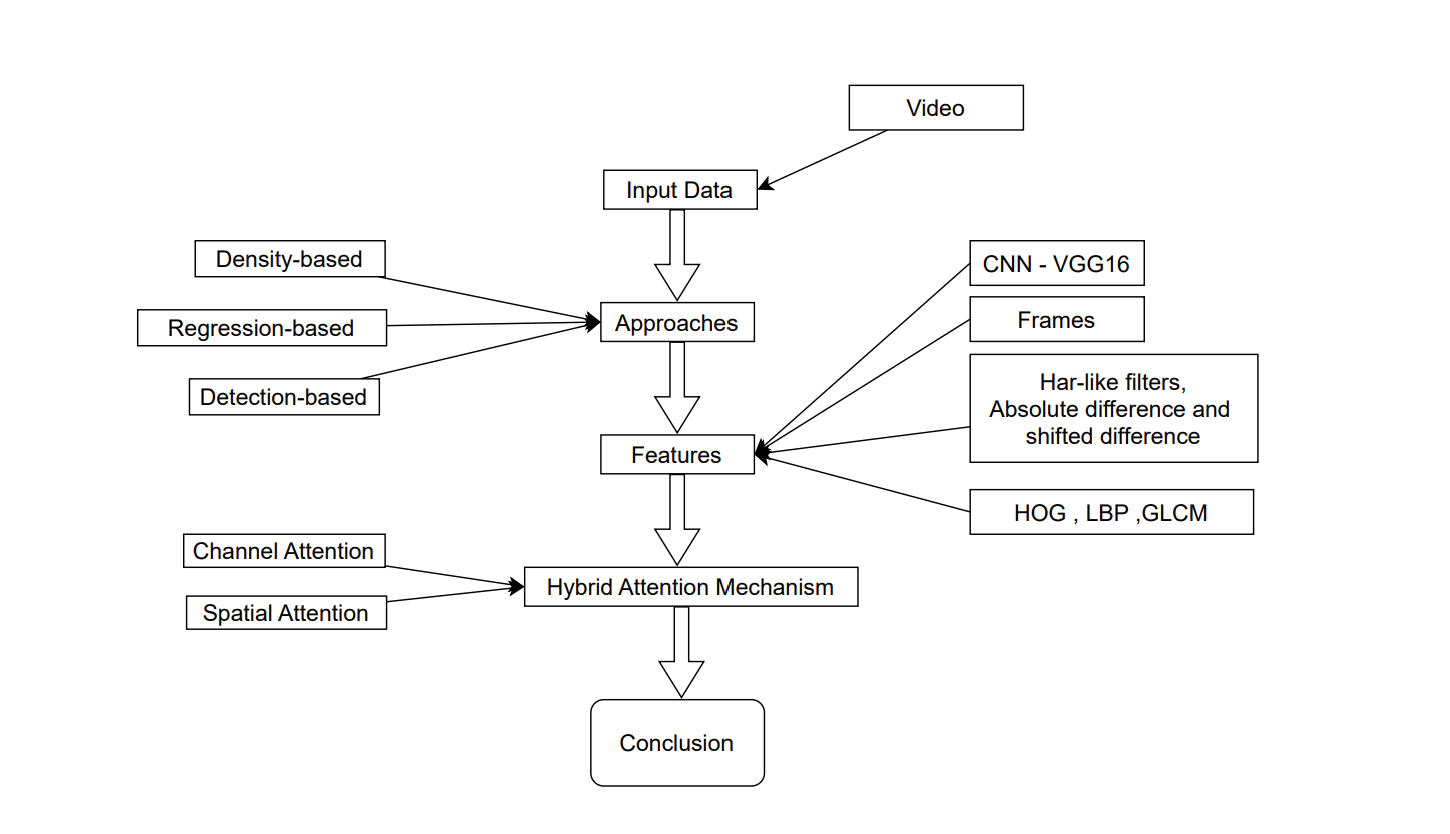
\includegraphics [width=0.9\textwidth, height=9cm]{Workflow.png}
  \caption{General Work Flow of Crowd Detection System using HAM}
  \label{fig:image}
\end{figure}

By following this workflow, the project aims to deliver a robust and efficient crowd-counting system that can be deployed in various practical applications. The combination of CNN and attention mechanisms enhance the accuracy and reliability of the system, making it a valuable tool for safety management, video surveillance, and urban planning.
\newline

% Section 4 of Chapter 3
\section{Implementation}

The implementation of the project was done using the Python programming language and the Django web framework. The project was developed as a web application, which allowed the user to upload a video file to the server. The video file was then processed using the proposed method of crowd counting, and the output was displayed to the user in the form of a crowd count.
\newline

The implementation consisted of several modules, each responsible for a specific task in the crowd-counting process. The first module was responsible for collecting the data set of images and videos, which was used for training and evaluation of the crowd-counting model. The data set consisted of a large number of images and videos captured in crowded environments, which provided a diverse range of crowd distributions.
\newline

The next module in the implementation was the image processing module, which converted the uploaded video to grayscale and performed feature extraction on each frame of the video. The features were then used to cluster and classify the pixels in the frame into regions corresponding to individual heads. The heads were then counted using a hybrid attention mechanism, which fused the content extracted from different regions of the frame to produce an accurate count of the heads.
\newline

The headcount was then aggregated across all the frames of the video to produce the final crowd count. The implementation used a combination of deep learning models and traditional computer vision techniques to achieve high accuracy in crowd counting. The input data was trained using regularization techniques to avoid overfitting and achieve generalization across different crowd distributions.
\newline

The evaluation module was used to evaluate the performance of the crowd-counting model on a separate test set of images and videos. The model was fine-tuned based on the results of the evaluation to improve its accuracy.
\newline

The web application was deployed using the Django web framework, which provided a user-friendly interface for uploading the video file and viewing the crowd count output. The implementation of the project demonstrated the effectiveness of the proposed method for crowd counting in real-world scenarios, and its potential applications in safety management, video surveillance, and urban planning.
\newline



% Chapter 4
\chapter{Agile Methodology}

% Section 1 of Chapter 4
\section{Introduction}

Agile methodology was used in the development of the crowd-counting project. The Agile approach is an iterative and incremental method of project management that emphasizes flexibility, collaboration, and customer satisfaction. It was adopted to ensure that the project could be executed in an efficient and effective manner, with the ability to adapt to changing requirements or unforeseen challenges. The development team used the Scrum framework, which is a popular Agile methodology that emphasizes frequent and short development cycles called sprints.
\newline \newline
The Scrum team was composed of developers, a project manager, and a product owner. The product owner was responsible for defining the project requirements and prioritizing the product backlog. The team held daily stand-up meetings to discuss progress, address issues, and plan the next steps. The team used an online project management tool to manage the backlog, track progress, and communicate with each other.
\newline \newline
Each sprint had a defined set of goals, which were outlined in the sprint backlog. At the end of each sprint, the team delivered a working increment of the project, which was demonstrated to the product owner for review and feedback. The product owner provided feedback and prioritized the next set of features for the upcoming sprints.
\newline \newline
The Agile approach allowed the development team to quickly respond to feedback and make changes to the project as needed. It also provided a framework for the team to work collaboratively and deliver high-quality software in a timely manner. The use of Agile methodology was instrumental in the successful completion of the project.
\newline


% Section 2 of Chapter 4
\section{User Story}

A user story is a concise, high-level description of a feature or functionality of a product that is written from the perspective of the user or customer. It is used to capture the user's needs, goals, and desired outcomes, rather than specifying the technical details of how the feature will be implemented. User stories are a key component of agile software development methodologies, which emphasize collaboration and responding to change over following a rigid plan.\newline \newline
User stories typically follow a simple format, such as "As a [user], I want [goal], so that [benefit]." The user story describes a specific feature or functionality that the user needs to achieve a particular goal or outcome. By focusing on the user's needs and goals, user stories help ensure that development efforts are aligned with the user's needs and that the resulting product is more likely to be useful and valuable.\newline \newline
User stories are often written on index cards or sticky notes and can be easily prioritized and organized by the development team. They are used to drive the development process, helping to ensure that the team is building features and functionality that are aligned with the user's needs. As the product evolves and new requirements emerge, user stories can be added, updated, or removed, allowing the team to respond quickly and effectively to changing circumstances. Overall, user stories are an important tool for building better products that meet the needs and goals of the end users. The user story of the system is given in Table 4.1 and Table 4.2
\newline

\arrayrulecolor{black}
\newcolumntype{P}[1]{>{\centering\arraybackslash}p{#1}}
\begin{table}[htbp]
\renewcommand{\arraystretch}{1.75} % Increase vertical spacing between rows
  \centering
  \setlength{\tabcolsep}{6pt}
 % \rowcolors{2}{gray!25}{white}
\begin{tabular}{ !{\vrule width 1pt} p{1.5cm} !{\vrule width 1pt} p{2cm} !{\vrule width 1pt} p{5cm} !{\vrule width 1pt} p{6cm} !{\vrule width 1pt} }
   \Xhline{3\arrayrulewidth} 
 \rowcolor{yellow!30}  \textbf{User Story ID} & \textbf{As a type of User} & \textbf{I want to do\newline (Perform some of the task)} & \textbf{So that I can\newline (Achieve Some Goal)} \\
   \Xhline{3\arrayrulewidth}
	 1  & HAM USER   &  Collect the Data Set  &  Collecting different videos of containing of crowd scenarios \\
  \hline
	 2  &  HAM USER &  Image Processing &  Resizing the images to a fixed size, normalizing the pixel values \\
  \hline
	 3  &  HAM USER &  Converting to grayscale &  The images were converted to grayscale to reduce the computational cost of the model \\
  \hline
	 4  &  HAM USER &  Feature Extraction &  Extract high-level features from the input images or frames \\
  \hline
	 5  &  HAM USER &  Data Clustering and Classification &  Splitting the dataset into training and validation sets, the height, width, and number of channels of the feature map \\
  \hline
	 6  &  HAM USER &  Hybrid Attention mechanism &  Apply a hybrid attention mechanism to the feature map to focus on the most informative regions of the image or frame \\
  \hline
	 7  &  HAM USER &  Collecting the headcount &  After applying the HAM and from that the informative part is captured to get the headcount from the crowd \\
  \Xhline{3\arrayrulewidth}
\end{tabular}
\caption{User Story: 1}
\label{tab:mytable}
\end{table}

\arrayrulecolor{black}
\newcolumntype{P}[1]{>{\centering\arraybackslash}p{#1}}
\begin{table}
\renewcommand{\arraystretch}{1.75} % Increase vertical spacing between rows
  \centering
  \setlength{\tabcolsep}{6pt}
 % \rowcolors{2}{gray!25}{white}
\begin{tabular}{ !{\vrule width 1pt} p{1.5cm} !{\vrule width 1pt} p{2cm} !{\vrule width 1pt} p{5cm} !{\vrule width 1pt} p{6cm} !{\vrule width 1pt} }
   \Xhline{3\arrayrulewidth} 
  \rowcolor{yellow!30} \textbf{User Story ID} & \textbf{As a type of User} & \textbf{I want to do\newline (Perform some of the task)} & \textbf{So that I can\newline (Achieve Some Goal)} \\
   \Xhline{3\arrayrulewidth}
	 8  &  HAM USER &  Crowd Counting &  Use a regression model to estimate the number of individuals in the attended feature map \\
  \hline
	 9  &  HAM USER &  Training the input data &  Train the model using a suitable dataset and validation set \\
  \hline
	 10  &  HAM USER &  Regularizing the data &  Models in order to minimize the adjusted loss function and prevent overfitting or underfitting \\
  \hline
	 11  &  HAM USER  &  Evaluation  &  Evaluate the performance of the model on a test set using appropriate metrics, such as mean absolute error or mean squared error \\
  \hline
	 12  &  HAM USER &  Creating the count &  After completing the evaluation there produce the crowd \\
  \hline
	 13  &  HAM USER &  Fine-Tuning  &  Using the weights of an already trained network as the starting values for training a new network \\
  \hline
	 14  &  HAM USER &  Count Produced  &  The weight produced is been converted to the count of the crowd \\
  \Xhline{3\arrayrulewidth}
\end{tabular}
\caption{User Story: 2}
\label{tab:mytable}
\end{table}


% Section 3 of Chapter 4
\section{Product Backlog}

The product backlog is a prioritized list of requirements or features that need to be developed for a product. It is a key artifact in agile software development methodologies, such as Scrum, and serves as the single source of truth for all the work that needs to be done on the product.\newline \newline
The product backlog is typically owned by the product owner, who is responsible for prioritizing the items on the backlog based on the needs and goals of the stakeholders. The items on the backlog are typically user stories, which describe the product's features or functionality from the user's perspective.\newline \newline
The product backlog is dynamic and evolves as new information becomes available or as the product evolves. Items can be added, removed, or reprioritized based on feedback from stakeholders, changes in the market or technology, or other factors. The development team uses the product backlog to plan and execute their work, pulling items from the top of the backlog into each sprint or development cycle. The product backlog of the system is given in Table 4.3 
\newline

\begin{table}[htbp]
\renewcommand{\arraystretch}{1.75} % Increase vertical spacing between rows
\centering
\begin{center}

\begin{tabular} { | p {1 cm} | p {4 cm} | p {3.5 cm} | p {2 cm} |p {3 cm} | }
 \hline
   \rowcolor{gray!30} \bfseries ID & \bfseries Name & \bfseries Priority\newline(High/Medium \newline /Low) &  \bfseries Estimate \newline (Hr) & \bfseries Status
(Planned/ \newline Progressing/ Completed)   \\
    \hline
    1 &Dataset Preparation & High & 34 & COMPLETED \\  \hline
    2 &Pre-processing & High & 40 & COMPLETED \\  \hline
    3 &Feature Extraction & High & 32 & COMPLETED \\  \hline
    4 &Data Clustering and Classification & High & 38 & COMPLETED \\  \hline
    5 & Hybrid Attention Mechanism & High & 54 & COMPLETED \\  \hline
    6 & Crowd Counting & High & 50 & COMPLETED \\  \hline
    7 & Training & High & 44 & COMPLETED \\  \hline
    8 & Evaluation & High & 32 & COMPLETED \\  \hline

\end{tabular}
\caption{Product Backlog}
\label{tab:mytable}
\end{center}
\end{table}


% Section 4 of Chapter 4
\section{Project Plan}

A project plan is a detailed document that outlines the objectives, tasks, timelines, resources, and potential risks associated with a specific project. It serves as a roadmap that guides the project team in successfully executing and completing the project within the defined constraints, such as budget, timeline, and scope. \newline \newline
A project plan is critical for ensuring that a project is completed efficiently, effectively, and on time. It helps project managers and team members stay focused on the project goals and objectives and provides a framework for managing tasks, timelines, and resources. A well-defined project plan also helps identify potential risks and challenges, allowing project teams to prepare and implement appropriate strategies to mitigate them. Ultimately, a project plan is essential for managing a project and ensuring that it meets or exceeds stakeholders' expectations. The project plan of the system is given in Table 4.4
\newline

\begin{table}[htbp]
\centering
\begin{tblr}{
  cell{2}{2} = {r=4}{},
  cell{6}{2} = {r=3}{},
  cell{9}{2} = {r=4}{},
  cell{13}{2} = {r=3}{},
  vlines,
  hline{1,2-5,6-8,9-12,13-15,16} = {-}{},
  hline{1,5,8,12,15} = {1,3-6}{},
  row{1}={bg=red},
  row{2}={bg=white},
  row{3}={bg=white},
  row{4}={bg=white},
  row{5}={bg=white},
  row{6}={bg=gray!30},
  row{7}={bg=gray!30},
  row{8}={bg=gray!30},
  row{9}={bg=white},
  row{10}={bg=white},
  row{11}={bg=white},
  row{12}={bg=white},
  row{13}={bg=gray!30},
  row{14}={bg=gray!30},
  row{15}={bg=gray!30},
}
{\textbf{User }\\\textbf{Story }\\\textbf{ID}}& \textbf{Task Name} & \textbf{Start Date} & \textbf{End Date} &\textbf{Days} & \textbf{Status}  \\
1 & Sprint 1 & 01/02/2023 & 07/02/2023 & 7 DAYS & Completed  \\
2 & Sprint 1 & 08/02/2023 & 13/02/2023 & 6 DAYS & Completed  \\
3 &Sprint 1 & 14/02/2023 & 17/02/2023 & 4 DAYS & Completed \\
4 & Sprint 1 & 18/02/2023 & 21/02/2023 & 4 DAYS & Completed \\
5 & Sprint 2 & 27/02/2023 & 05/03/2023 & 7 DAYS & Completed \\
6 & Sprint 2 & 06/03/2023 & 12/03/2023 & 7 DAYS & Completed \\
7 & Sprint 2 & 14/03/2023 & 20/03/2023 & 7 DAYS  & Completed \\
8 & Sprint 3 & 22/03/2023 & 27/03/2023 & 6 DAYS & Completed \\
9 & Sprint 3 & 28/03/2023 & 31/03/2023 & 4 DAYS & Completed \\
10 & Sprint 3 & 01/04/2023 & 05/04/2023 & 5 DAYS & Completed \\
11 & Sprint 3 & 06/04/2023 & 11/04/2023 & 6 DAYS & Completed \\
12 & Sprint 4 & 15/04/2023 & 22/04/2023 & 8 DAYS & Completed \\
13 & Sprint 4 & 23/04/2023 & 01/04/2023 & 9 DAYS & Completed \\
14 & Sprint 4 & 02/04/2023 & 05/04/2023 & 4 DAYS & Completed \\
\end{tblr}
\caption{Project Plan}
\label{tab:mytable}
\end{table}


% Section 5 of Chapter 4
\section{Sprint Backlog (Plan)}

The Sprint Backlog is a plan created by the Development Team at the beginning of each Sprint. It details the work that needs to be completed during the Sprint to meet the Sprint Goal. The Sprint Backlog is created during the Sprint Planning event, where the Development Team decides on the work that will be completed during the Sprint. The Product Owner presents the Product Backlog items they want to be completed during the Sprint, and the Development Team determines how much work they can realistically complete during the Sprint. The detailed sprint backlog (Plan) is given below.
\newline

\begin{table}[h]
\LARGE
\resizebox{\textwidth}{!}{%
\centering
\begin{tabular}{|cc|cccccccc|}
\hline
\rowcolor[HTML]{96FFFB} 
\multicolumn{1}{|c|}{\cellcolor[HTML]{96FFFB}\textbf{\begin{tabular}[c]{@{}c@{}}Backlog\\ Item\end{tabular}}}    & \textbf{\begin{tabular}[c]{@{}c@{}}Completion\\ date\end{tabular}} & \multicolumn{1}{c|}{\cellcolor[HTML]{96FFFB}\textbf{\begin{tabular}[c]{@{}c@{}}Original\\ estimate\end{tabular}}} & \multicolumn{1}{c|}{\cellcolor[HTML]{96FFFB}\textbf{\begin{tabular}[c]{@{}c@{}}Day 1\\ 01/02/23\end{tabular}}} & \multicolumn{1}{c|}{\cellcolor[HTML]{96FFFB}\textbf{\begin{tabular}[c]{@{}c@{}}Day 2\\ 02/02/23\end{tabular}}} & \multicolumn{1}{c|}{\cellcolor[HTML]{96FFFB}\textbf{\begin{tabular}[c]{@{}c@{}}Day 3\\ 03/02/23\end{tabular}}} & \multicolumn{1}{c|}{\cellcolor[HTML]{96FFFB}\textbf{\begin{tabular}[c]{@{}c@{}}Day 4\\ 04/02/23\end{tabular}}} & \multicolumn{1}{c|}{\cellcolor[HTML]{96FFFB}\textbf{\begin{tabular}[c]{@{}c@{}}Day 5\\ 05/02/23\end{tabular}}} & \multicolumn{1}{c|}{\cellcolor[HTML]{96FFFB}\textbf{\begin{tabular}[c]{@{}c@{}}Day 6\\ 06/02/23\end{tabular}}} & \textbf{\begin{tabular}[c]{@{}c@{}}Day 7\\ 07/02/23\end{tabular}} \\ \hline
\rowcolor[HTML]{96FFFB} 
\multicolumn{1}{|c|}{\cellcolor[HTML]{96FFFB}\textbf{\begin{tabular}[c]{@{}c@{}}User \\ Story \#1\end{tabular}}} &                                                                    & \multicolumn{1}{c|}{\cellcolor[HTML]{96FFFB}Hours}                                                                & \multicolumn{1}{c|}{\cellcolor[HTML]{96FFFB}Hours}                                                             & \multicolumn{1}{c|}{\cellcolor[HTML]{96FFFB}Hours}                                                             & \multicolumn{1}{c|}{\cellcolor[HTML]{96FFFB}Hours}                                                             & \multicolumn{1}{c|}{\cellcolor[HTML]{96FFFB}Hours}                                                             & \multicolumn{1}{c|}{\cellcolor[HTML]{96FFFB}Hours}                                                             & \multicolumn{1}{c|}{\cellcolor[HTML]{96FFFB}Hours}                                                             & Hours                                                             \\ \hline
\rowcolor[HTML]{FFFFFF} 
\multicolumn{1}{|c|}{\cellcolor[HTML]{FFFFFF}\textbf{\begin{tabular}[c]{@{}c@{}}Form\\ Designing\end{tabular}}}  & 02/02/23                                                           & \multicolumn{1}{c|}{\cellcolor[HTML]{FFFFFF}2}                                                                    & \multicolumn{1}{c|}{\cellcolor[HTML]{FFFFFF}1}                                                                 & \multicolumn{1}{c|}{\cellcolor[HTML]{FFFFFF}1}                                                                 & \multicolumn{1}{c|}{\cellcolor[HTML]{FFFFFF}0}                                                                 & \multicolumn{1}{c|}{\cellcolor[HTML]{FFFFFF}0}                                                                 & \multicolumn{1}{c|}{\cellcolor[HTML]{FFFFFF}0}                                                                 & \multicolumn{1}{c|}{\cellcolor[HTML]{FFFFFF}0}                                                                 & \cellcolor[HTML]{FFFFFF}0                                         \\ \hline
\rowcolor[HTML]{FFFFFF} 
\multicolumn{1}{|c|}{\cellcolor[HTML]{FFFFFF}\textbf{Coding}}                                                    & 07/02/23                                                           & \multicolumn{1}{c|}{\cellcolor[HTML]{FFFFFF}33}                                                                   & \multicolumn{1}{c|}{\cellcolor[HTML]{FFFFFF}1}                                                                 & \multicolumn{1}{c|}{\cellcolor[HTML]{FFFFFF}3}                                                                 & \multicolumn{1}{c|}{\cellcolor[HTML]{FFFFFF}6}                                                                 & \multicolumn{1}{c|}{\cellcolor[HTML]{FFFFFF}6}                                                                 & \multicolumn{1}{c|}{\cellcolor[HTML]{FFFFFF}6}                                                                 & \multicolumn{1}{c|}{\cellcolor[HTML]{FFFFFF}6}                                                                 & \cellcolor[HTML]{FFFFFF}5                                         \\ \hline
\rowcolor[HTML]{FFFFFF} 
\multicolumn{1}{|c|}{\cellcolor[HTML]{FFFFFF}\textbf{Testing}}                                                   & 07/02/23                                                           & \multicolumn{1}{c|}{\cellcolor[HTML]{FFFFFF}1}                                                                    & \multicolumn{1}{c|}{\cellcolor[HTML]{FFFFFF}0}                                                                 & \multicolumn{1}{c|}{\cellcolor[HTML]{FFFFFF}0}                                                                 & \multicolumn{1}{c|}{\cellcolor[HTML]{FFFFFF}0}                                                                 & \multicolumn{1}{c|}{\cellcolor[HTML]{FFFFFF}0}                                                                 & \multicolumn{1}{c|}{\cellcolor[HTML]{FFFFFF}0}                                                                 & \multicolumn{1}{c|}{\cellcolor[HTML]{FFFFFF}0}                                                                 & \cellcolor[HTML]{FFFFFF}1                                         \\ \hline
\multicolumn{2}{|c|}{\textbf{Total}}                                                                                                                                                  & \multicolumn{8}{c|}{36   Hours}                                                                                                                                                                                                                                                                                                                                                                                                                                                                                                                                                                                                                                                                                                                                                                                                                                                             \\ \hline
\end{tabular}
}
\caption{Sprint Backlog1 (Plan) User Story 1}
\label{tab:mytable}
\end{table}


\begin{table}[h]
\LARGE
\resizebox{\textwidth}{!}{%
\centering
\begin{tabular}{|cc|ccccccc|}
\hline
\rowcolor[HTML]{96FFFB} 
\multicolumn{1}{|c|}{\cellcolor[HTML]{96FFFB}\textbf{\begin{tabular}[c]{@{}c@{}}Backlog\\ Item\end{tabular}}}    & \textbf{\begin{tabular}[c]{@{}c@{}}Completion\\ date\end{tabular}} & \multicolumn{1}{c|}{\cellcolor[HTML]{96FFFB}\textbf{\begin{tabular}[c]{@{}c@{}}Original\\ estimate\end{tabular}}} & \multicolumn{1}{c|}{\cellcolor[HTML]{96FFFB}\textbf{\begin{tabular}[c]{@{}c@{}}Day 8\\ 08/02/23\end{tabular}}} & \multicolumn{1}{c|}{\cellcolor[HTML]{96FFFB}\textbf{\begin{tabular}[c]{@{}c@{}}Day 9\\ 09/02/23\end{tabular}}} & \multicolumn{1}{c|}{\cellcolor[HTML]{96FFFB}\textbf{\begin{tabular}[c]{@{}c@{}}Day 10\\ 10/02/23\end{tabular}}} & \multicolumn{1}{c|}{\cellcolor[HTML]{96FFFB}\textbf{\begin{tabular}[c]{@{}c@{}}Day 11\\ 11/02/23\end{tabular}}} & \multicolumn{1}{c|}{\cellcolor[HTML]{96FFFB}\textbf{\begin{tabular}[c]{@{}c@{}}Day 12\\ 12/02/23\end{tabular}}} & \textbf{\begin{tabular}[c]{@{}c@{}}Day 13\\ 13/02/23\end{tabular}} \\ \hline
\rowcolor[HTML]{96FFFB} 
\multicolumn{1}{|c|}{\cellcolor[HTML]{96FFFB}\textbf{\begin{tabular}[c]{@{}c@{}}User \\ Story \#2\end{tabular}}} &                                                                    & \multicolumn{1}{c|}{\cellcolor[HTML]{96FFFB}Hours}                                                                & \multicolumn{1}{c|}{\cellcolor[HTML]{96FFFB}Hours}                                                             & \multicolumn{1}{c|}{\cellcolor[HTML]{96FFFB}Hours}                                                             & \multicolumn{1}{c|}{\cellcolor[HTML]{96FFFB}Hours}                                                              & \multicolumn{1}{c|}{\cellcolor[HTML]{96FFFB}Hours}                                                              & \multicolumn{1}{c|}{\cellcolor[HTML]{96FFFB}Hours}                                                              & Hours                                                              \\ \hline
\rowcolor[HTML]{FFFFFF} 
\multicolumn{1}{|c|}{\cellcolor[HTML]{FFFFFF}\textbf{\begin{tabular}[c]{@{}c@{}}Form\\ Designing\end{tabular}}}  & 08/02/23                                                           & \multicolumn{1}{c|}{\cellcolor[HTML]{FFFFFF}1}                                                                    & \multicolumn{1}{c|}{\cellcolor[HTML]{FFFFFF}1}                                                                 & \multicolumn{1}{c|}{\cellcolor[HTML]{FFFFFF}0}                                                                 & \multicolumn{1}{c|}{\cellcolor[HTML]{FFFFFF}0}                                                                  & \multicolumn{1}{c|}{\cellcolor[HTML]{FFFFFF}0}                                                                  & \multicolumn{1}{c|}{\cellcolor[HTML]{FFFFFF}0}                                                                  & \cellcolor[HTML]{FFFFFF}0                                          \\ \hline
\rowcolor[HTML]{FFFFFF} 
\multicolumn{1}{|c|}{\cellcolor[HTML]{FFFFFF}\textbf{Coding}}                                                    & 07/02/23                                                           & \multicolumn{1}{c|}{\cellcolor[HTML]{FFFFFF}28}                                                                   & \multicolumn{1}{c|}{\cellcolor[HTML]{FFFFFF}4}                                                                 & \multicolumn{1}{c|}{\cellcolor[HTML]{FFFFFF}5}                                                                 & \multicolumn{1}{c|}{\cellcolor[HTML]{FFFFFF}5}                                                                  & \multicolumn{1}{c|}{\cellcolor[HTML]{FFFFFF}5}                                                                  & \multicolumn{1}{c|}{\cellcolor[HTML]{FFFFFF}5}                                                                  & \cellcolor[HTML]{FFFFFF}4                                          \\ \hline
\rowcolor[HTML]{FFFFFF} 
\multicolumn{1}{|c|}{\cellcolor[HTML]{FFFFFF}\textbf{Testing}}                                                   & 13/02/23                                                           & \multicolumn{1}{c|}{\cellcolor[HTML]{FFFFFF}1}                                                                    & \multicolumn{1}{c|}{\cellcolor[HTML]{FFFFFF}0}                                                                 & \multicolumn{1}{c|}{\cellcolor[HTML]{FFFFFF}0}                                                                 & \multicolumn{1}{c|}{\cellcolor[HTML]{FFFFFF}0}                                                                  & \multicolumn{1}{c|}{\cellcolor[HTML]{FFFFFF}0}                                                                  & \multicolumn{1}{c|}{\cellcolor[HTML]{FFFFFF}0}                                                                  & \cellcolor[HTML]{FFFFFF}1                                          \\ \hline
\multicolumn{2}{|c|}{\textbf{Total}}                                                                                                                                                  & \multicolumn{7}{c|}{30   Hours}                                                                                                                                                                                                                                                                                                                                                                                                                                                                                                                                                                                                                                                                                                                                                \\ \hline
\end{tabular}
}
\caption{Sprint Backlog1 (Plan) User Story 2}
\label{tab:mytable}
\end{table}


{\small
\begin{table}[]
\centering
\begin{tabular}{|cc|ccccc|}
\hline
\rowcolor[HTML]{96FFFB} 
\multicolumn{1}{|c|}{\cellcolor[HTML]{96FFFB}\textbf{\begin{tabular}[c]{@{}c@{}}Backlog\\ Item\end{tabular}}}    & \textbf{\begin{tabular}[c]{@{}c@{}}Completion\\ date\end{tabular}} & \multicolumn{1}{c|}{\cellcolor[HTML]{96FFFB}\textbf{\begin{tabular}[c]{@{}c@{}}Original\\ estimate\end{tabular}}} & \multicolumn{1}{c|}{\cellcolor[HTML]{96FFFB}\textbf{\begin{tabular}[c]{@{}c@{}}Day 14\\ 14/02/23\end{tabular}}} & \multicolumn{1}{c|}{\cellcolor[HTML]{96FFFB}\textbf{\begin{tabular}[c]{@{}c@{}}Day 15\\ 15/02/23\end{tabular}}} & \multicolumn{1}{c|}{\cellcolor[HTML]{96FFFB}\textbf{\begin{tabular}[c]{@{}c@{}}Day 16\\ 16/02/23\end{tabular}}} & \textbf{\begin{tabular}[c]{@{}c@{}}Day 17\\ 17/02/23\end{tabular}} \\ \hline
\rowcolor[HTML]{96FFFB} 
\multicolumn{1}{|c|}{\cellcolor[HTML]{96FFFB}\textbf{\begin{tabular}[c]{@{}c@{}}User \\ Story \#3\end{tabular}}} &                                                                    & \multicolumn{1}{c|}{\cellcolor[HTML]{96FFFB}Hours}                                                                & \multicolumn{1}{c|}{\cellcolor[HTML]{96FFFB}Hours}                                                              & \multicolumn{1}{c|}{\cellcolor[HTML]{96FFFB}Hours}                                                              & \multicolumn{1}{c|}{\cellcolor[HTML]{96FFFB}Hours}                                                              & Hours                                                              \\ \hline
\rowcolor[HTML]{FFFFFF} 
\multicolumn{1}{|c|}{\cellcolor[HTML]{FFFFFF}\textbf{\begin{tabular}[c]{@{}c@{}}Form\\ Designing\end{tabular}}}  & 14/02/23                                                           & \multicolumn{1}{c|}{\cellcolor[HTML]{FFFFFF}1}                                                                    & \multicolumn{1}{c|}{\cellcolor[HTML]{FFFFFF}1}                                                                  & \multicolumn{1}{c|}{\cellcolor[HTML]{FFFFFF}0}                                                                  & \multicolumn{1}{c|}{\cellcolor[HTML]{FFFFFF}0}                                                                  & \cellcolor[HTML]{FFFFFF}0                                          \\ \hline
\rowcolor[HTML]{FFFFFF} 
\multicolumn{1}{|c|}{\cellcolor[HTML]{FFFFFF}\textbf{Coding}}                                                    & 07/02/23                                                           & \multicolumn{1}{c|}{\cellcolor[HTML]{FFFFFF}18}                                                                   & \multicolumn{1}{c|}{\cellcolor[HTML]{FFFFFF}4}                                                                  & \multicolumn{1}{c|}{\cellcolor[HTML]{FFFFFF}5}                                                                  & \multicolumn{1}{c|}{\cellcolor[HTML]{FFFFFF}5}                                                                  & \cellcolor[HTML]{FFFFFF}4                                          \\ \hline
\rowcolor[HTML]{FFFFFF} 
\multicolumn{1}{|c|}{\cellcolor[HTML]{FFFFFF}\textbf{Testing}}                                                   & 17/02/23                                                           & \multicolumn{1}{c|}{\cellcolor[HTML]{FFFFFF}1}                                                                    & \multicolumn{1}{c|}{\cellcolor[HTML]{FFFFFF}0}                                                                  & \multicolumn{1}{c|}{\cellcolor[HTML]{FFFFFF}0}                                                                  & \multicolumn{1}{c|}{\cellcolor[HTML]{FFFFFF}0}                                                                  & \cellcolor[HTML]{FFFFFF}1                                          \\ \hline
\multicolumn{2}{|c|}{\textbf{Total}}                                                                                                                                                  & \multicolumn{5}{c|}{20   Hours}                                                                                                                                                                                                                                                                                                                                                                                                                                                                                                              \\ \hline
\end{tabular}
\caption{Sprint Backlog1 (Plan) User Story 3}
\label{tab:mytable}
\end{table}
}


{\small
\begin{table}[]
\centering
\begin{tabular}{|cc|ccccc|}
\hline
\rowcolor[HTML]{96FFFB} 
\multicolumn{1}{|c|}{\cellcolor[HTML]{96FFFB}\textbf{\begin{tabular}[c]{@{}c@{}}Backlog\\ Item\end{tabular}}}    & \textbf{\begin{tabular}[c]{@{}c@{}}Completion\\ date\end{tabular}} & \multicolumn{1}{c|}{\cellcolor[HTML]{96FFFB}\textbf{\begin{tabular}[c]{@{}c@{}}Original\\ estimate\end{tabular}}} & \multicolumn{1}{c|}{\cellcolor[HTML]{96FFFB}\textbf{\begin{tabular}[c]{@{}c@{}}Day 18\\ 18/02/23\end{tabular}}} & \multicolumn{1}{c|}{\cellcolor[HTML]{96FFFB}\textbf{\begin{tabular}[c]{@{}c@{}}Day 19\\ 19/02/23\end{tabular}}} & \multicolumn{1}{c|}{\cellcolor[HTML]{96FFFB}\textbf{\begin{tabular}[c]{@{}c@{}}Day 20\\ 20/02/23\end{tabular}}} & \textbf{\begin{tabular}[c]{@{}c@{}}Day 21\\ 21/02/23\end{tabular}} \\ \hline
\rowcolor[HTML]{96FFFB} 
\multicolumn{1}{|c|}{\cellcolor[HTML]{96FFFB}\textbf{\begin{tabular}[c]{@{}c@{}}User \\ Story \#4\end{tabular}}} &                                                                    & \multicolumn{1}{c|}{\cellcolor[HTML]{96FFFB}Hours}                                                                & \multicolumn{1}{c|}{\cellcolor[HTML]{96FFFB}Hours}                                                              & \multicolumn{1}{c|}{\cellcolor[HTML]{96FFFB}Hours}                                                              & \multicolumn{1}{c|}{\cellcolor[HTML]{96FFFB}Hours}                                                              & Hours                                                              \\ \hline
\rowcolor[HTML]{FFFFFF} 
\multicolumn{1}{|c|}{\cellcolor[HTML]{FFFFFF}\textbf{\begin{tabular}[c]{@{}c@{}}Form\\ Designing\end{tabular}}}  & 18/02/23                                                           & \multicolumn{1}{c|}{\cellcolor[HTML]{FFFFFF}1}                                                                    & \multicolumn{1}{c|}{\cellcolor[HTML]{FFFFFF}1}                                                                  & \multicolumn{1}{c|}{\cellcolor[HTML]{FFFFFF}0}                                                                  & \multicolumn{1}{c|}{\cellcolor[HTML]{FFFFFF}0}                                                                  & \cellcolor[HTML]{FFFFFF}0                                          \\ \hline
\rowcolor[HTML]{FFFFFF} 
\multicolumn{1}{|c|}{\cellcolor[HTML]{FFFFFF}\textbf{Coding}}                                                    & 21/02/23                                                           & \multicolumn{1}{c|}{\cellcolor[HTML]{FFFFFF}18}                                                                   & \multicolumn{1}{c|}{\cellcolor[HTML]{FFFFFF}4}                                                                  & \multicolumn{1}{c|}{\cellcolor[HTML]{FFFFFF}5}                                                                  & \multicolumn{1}{c|}{\cellcolor[HTML]{FFFFFF}5}                                                                  & \cellcolor[HTML]{FFFFFF}4                                          \\ \hline
\rowcolor[HTML]{FFFFFF} 
\multicolumn{1}{|c|}{\cellcolor[HTML]{FFFFFF}\textbf{Testing}}                                                   & 21/02/23                                                           & \multicolumn{1}{c|}{\cellcolor[HTML]{FFFFFF}1}                                                                    & \multicolumn{1}{c|}{\cellcolor[HTML]{FFFFFF}0}                                                                  & \multicolumn{1}{c|}{\cellcolor[HTML]{FFFFFF}0}                                                                  & \multicolumn{1}{c|}{\cellcolor[HTML]{FFFFFF}0}                                                                  & \cellcolor[HTML]{FFFFFF}1                                          \\ \hline
\multicolumn{2}{|c|}{\textbf{Total}}                                                                                                                                                  & \multicolumn{5}{c|}{20   Hours}                                                                                                                                                                                                                                                                                                                                                                                                                                                                                                              \\ \hline
\end{tabular}
\caption{Sprint Backlog1 (Plan) User Story 4}
\label{tab:mytable}
\end{table}
}


\begin{table}[h]
\LARGE
\resizebox{\textwidth}{!}{%
\centering
\begin{tabular}{|cc|cccccccc|}
\hline
\rowcolor[HTML]{96FFFB} 
\multicolumn{1}{|c|}{\cellcolor[HTML]{96FFFB}\textbf{\begin{tabular}[c]{@{}c@{}}Backlog\\ Item\end{tabular}}}    & \textbf{\begin{tabular}[c]{@{}c@{}}Completion\\ date\end{tabular}} & \multicolumn{1}{c|}{\cellcolor[HTML]{96FFFB}\textbf{\begin{tabular}[c]{@{}c@{}}Original\\ estimate\end{tabular}}} & \multicolumn{1}{c|}{\cellcolor[HTML]{96FFFB}\textbf{\begin{tabular}[c]{@{}c@{}}Day 22\\ 27/02/23\end{tabular}}} & \multicolumn{1}{c|}{\cellcolor[HTML]{96FFFB}\textbf{\begin{tabular}[c]{@{}c@{}}Day 23\\ 28/02/23\end{tabular}}} & \multicolumn{1}{c|}{\cellcolor[HTML]{96FFFB}\textbf{\begin{tabular}[c]{@{}c@{}}Day 24\\ 01/03/23\end{tabular}}} & \multicolumn{1}{c|}{\cellcolor[HTML]{96FFFB}\textbf{\begin{tabular}[c]{@{}c@{}}Day 25\\ 02/03/23\end{tabular}}} & \multicolumn{1}{c|}{\cellcolor[HTML]{96FFFB}\textbf{\begin{tabular}[c]{@{}c@{}}Day 26\\ 03/03/23\end{tabular}}} & \multicolumn{1}{c|}{\cellcolor[HTML]{96FFFB}\textbf{\begin{tabular}[c]{@{}c@{}}Day 27\\ 04/03/23\end{tabular}}} & \cellcolor[HTML]{96FFFB}\textbf{\begin{tabular}[c]{@{}c@{}}Day 28\\ 05/03/23\end{tabular}} \\ \hline
\rowcolor[HTML]{96FFFB} 
\multicolumn{1}{|c|}{\cellcolor[HTML]{96FFFB}\textbf{\begin{tabular}[c]{@{}c@{}}User \\ Story \#5\end{tabular}}} &                                                                    & \multicolumn{1}{c|}{\cellcolor[HTML]{96FFFB}Hours}                                                                & \multicolumn{1}{c|}{\cellcolor[HTML]{96FFFB}Hours}                                                              & \multicolumn{1}{c|}{\cellcolor[HTML]{96FFFB}Hours}                                                              & \multicolumn{1}{c|}{\cellcolor[HTML]{96FFFB}Hours}                                                              & \multicolumn{1}{c|}{\cellcolor[HTML]{96FFFB}Hours}                                                              & \multicolumn{1}{c|}{\cellcolor[HTML]{96FFFB}Hours}                                                              & \multicolumn{1}{c|}{\cellcolor[HTML]{96FFFB}Hours}                                                              & \cellcolor[HTML]{96FFFB}Hours                                                              \\ \hline
\rowcolor[HTML]{FFFFFF} 
\multicolumn{1}{|c|}{\cellcolor[HTML]{FFFFFF}\textbf{\begin{tabular}[c]{@{}c@{}}Form\\ Designing\end{tabular}}}  & 27/02/23                                                           & \multicolumn{1}{c|}{\cellcolor[HTML]{FFFFFF}1}                                                                    & \multicolumn{1}{c|}{\cellcolor[HTML]{FFFFFF}1}                                                                  & \multicolumn{1}{c|}{\cellcolor[HTML]{FFFFFF}0}                                                                  & \multicolumn{1}{c|}{\cellcolor[HTML]{FFFFFF}0}                                                                  & \multicolumn{1}{c|}{\cellcolor[HTML]{FFFFFF}0}                                                                  & \multicolumn{1}{c|}{\cellcolor[HTML]{FFFFFF}0}                                                                  & \multicolumn{1}{c|}{\cellcolor[HTML]{FFFFFF}0}                                                                  & \cellcolor[HTML]{FFFFFF}0                                                                  \\ \hline
\rowcolor[HTML]{FFFFFF} 
\multicolumn{1}{|c|}{\cellcolor[HTML]{FFFFFF}\textbf{Coding}}                                                    & 05/03/23                                                           & \multicolumn{1}{c|}{\cellcolor[HTML]{FFFFFF}29}                                                                   & \multicolumn{1}{c|}{\cellcolor[HTML]{FFFFFF}2}                                                                  & \multicolumn{1}{c|}{\cellcolor[HTML]{FFFFFF}5}                                                                  & \multicolumn{1}{c|}{\cellcolor[HTML]{FFFFFF}5}                                                                  & \multicolumn{1}{c|}{\cellcolor[HTML]{FFFFFF}5}                                                                  & \multicolumn{1}{c|}{\cellcolor[HTML]{FFFFFF}5}                                                                  & \multicolumn{1}{c|}{\cellcolor[HTML]{FFFFFF}5}                                                                  & \cellcolor[HTML]{FFFFFF}2                                                                  \\ \hline
\rowcolor[HTML]{FFFFFF} 
\multicolumn{1}{|c|}{\cellcolor[HTML]{FFFFFF}\textbf{Testing}}                                                   & 05/03/23                                                           & \multicolumn{1}{c|}{\cellcolor[HTML]{FFFFFF}1}                                                                    & \multicolumn{1}{c|}{\cellcolor[HTML]{FFFFFF}0}                                                                  & \multicolumn{1}{c|}{\cellcolor[HTML]{FFFFFF}0}                                                                  & \multicolumn{1}{c|}{\cellcolor[HTML]{FFFFFF}0}                                                                  & \multicolumn{1}{c|}{\cellcolor[HTML]{FFFFFF}1}                                                                  & \multicolumn{1}{c|}{\cellcolor[HTML]{FFFFFF}0}                                                                  & \multicolumn{1}{c|}{\cellcolor[HTML]{FFFFFF}0}                                                                  & \cellcolor[HTML]{FFFFFF}1                                                                  \\ \hline
\multicolumn{2}{|c|}{\textbf{Total}}                                                                                                                                                  & \multicolumn{8}{c|}{31   Hours}                                                                                                                                                                                                                                                                                                                                                                                                                                                                                                                                                                                                                                                                                                                                                                                                                                                                                            \\ \hline
\end{tabular}
}
\caption{Sprint Backlog2 (Plan) User Story 5}
\label{tab:mytable}
\end{table}


\begin{table}[h]
\LARGE
\resizebox{\textwidth}{!}{%
\centering
\begin{tabular}{|cc|cccccccc|}
\hline
\rowcolor[HTML]{96FFFB} 
\multicolumn{1}{|c|}{\cellcolor[HTML]{96FFFB}\textbf{\begin{tabular}[c]{@{}c@{}}Backlog\\ Item\end{tabular}}}    & \textbf{\begin{tabular}[c]{@{}c@{}}Completion\\ date\end{tabular}} & \multicolumn{1}{c|}{\cellcolor[HTML]{96FFFB}\textbf{\begin{tabular}[c]{@{}c@{}}Original\\ estimate\end{tabular}}} & \multicolumn{1}{c|}{\cellcolor[HTML]{96FFFB}\textbf{\begin{tabular}[c]{@{}c@{}}Day 29\\ 06/03/23\end{tabular}}} & \multicolumn{1}{c|}{\cellcolor[HTML]{96FFFB}\textbf{\begin{tabular}[c]{@{}c@{}}Day 30\\ 07/03/23\end{tabular}}} & \multicolumn{1}{c|}{\cellcolor[HTML]{96FFFB}\textbf{\begin{tabular}[c]{@{}c@{}}Day 31\\ 08/03/23\end{tabular}}} & \multicolumn{1}{c|}{\cellcolor[HTML]{96FFFB}\textbf{\begin{tabular}[c]{@{}c@{}}Day 32\\ 09/03/23\end{tabular}}} & \multicolumn{1}{c|}{\cellcolor[HTML]{96FFFB}\textbf{\begin{tabular}[c]{@{}c@{}}Day 33\\ 10/03/23\end{tabular}}} & \multicolumn{1}{c|}{\cellcolor[HTML]{96FFFB}\textbf{\begin{tabular}[c]{@{}c@{}}Day 34\\ 11/03/23\end{tabular}}} & \cellcolor[HTML]{96FFFB}\textbf{\begin{tabular}[c]{@{}c@{}}Day 35\\ 12/03/23\end{tabular}} \\ \hline
\rowcolor[HTML]{96FFFB} 
\multicolumn{1}{|c|}{\cellcolor[HTML]{96FFFB}\textbf{\begin{tabular}[c]{@{}c@{}}User \\ Story \#6\end{tabular}}} &                                                                    & \multicolumn{1}{c|}{\cellcolor[HTML]{96FFFB}Hours}                                                                & \multicolumn{1}{c|}{\cellcolor[HTML]{96FFFB}Hours}                                                              & \multicolumn{1}{c|}{\cellcolor[HTML]{96FFFB}Hours}                                                              & \multicolumn{1}{c|}{\cellcolor[HTML]{96FFFB}Hours}                                                              & \multicolumn{1}{c|}{\cellcolor[HTML]{96FFFB}Hours}                                                              & \multicolumn{1}{c|}{\cellcolor[HTML]{96FFFB}Hours}                                                              & \multicolumn{1}{c|}{\cellcolor[HTML]{96FFFB}Hours}                                                              & \cellcolor[HTML]{96FFFB}Hours                                                              \\ \hline
\rowcolor[HTML]{FFFFFF} 
\multicolumn{1}{|c|}{\cellcolor[HTML]{FFFFFF}\textbf{\begin{tabular}[c]{@{}c@{}}Form\\ Designing\end{tabular}}}  & 06/03/23                                                           & \multicolumn{1}{c|}{\cellcolor[HTML]{FFFFFF}1}                                                                    & \multicolumn{1}{c|}{\cellcolor[HTML]{FFFFFF}1}                                                                  & \multicolumn{1}{c|}{\cellcolor[HTML]{FFFFFF}0}                                                                  & \multicolumn{1}{c|}{\cellcolor[HTML]{FFFFFF}0}                                                                  & \multicolumn{1}{c|}{\cellcolor[HTML]{FFFFFF}0}                                                                  & \multicolumn{1}{c|}{\cellcolor[HTML]{FFFFFF}0}                                                                  & \multicolumn{1}{c|}{\cellcolor[HTML]{FFFFFF}0}                                                                  & \cellcolor[HTML]{FFFFFF}0                                                                  \\ \hline
\rowcolor[HTML]{FFFFFF} 
\multicolumn{1}{|c|}{\cellcolor[HTML]{FFFFFF}\textbf{Coding}}                                                    & 12/03/23                                                           & \multicolumn{1}{c|}{\cellcolor[HTML]{FFFFFF}29}                                                                   & \multicolumn{1}{c|}{\cellcolor[HTML]{FFFFFF}2}                                                                  & \multicolumn{1}{c|}{\cellcolor[HTML]{FFFFFF}5}                                                                  & \multicolumn{1}{c|}{\cellcolor[HTML]{FFFFFF}5}                                                                  & \multicolumn{1}{c|}{\cellcolor[HTML]{FFFFFF}5}                                                                  & \multicolumn{1}{c|}{\cellcolor[HTML]{FFFFFF}5}                                                                  & \multicolumn{1}{c|}{\cellcolor[HTML]{FFFFFF}5}                                                                  & \cellcolor[HTML]{FFFFFF}2                                                                  \\ \hline
\rowcolor[HTML]{FFFFFF} 
\multicolumn{1}{|c|}{\cellcolor[HTML]{FFFFFF}\textbf{Testing}}                                                   & 12/03/23                                                           & \multicolumn{1}{c|}{\cellcolor[HTML]{FFFFFF}1}                                                                    & \multicolumn{1}{c|}{\cellcolor[HTML]{FFFFFF}0}                                                                  & \multicolumn{1}{c|}{\cellcolor[HTML]{FFFFFF}0}                                                                  & \multicolumn{1}{c|}{\cellcolor[HTML]{FFFFFF}0}                                                                  & \multicolumn{1}{c|}{\cellcolor[HTML]{FFFFFF}1}                                                                  & \multicolumn{1}{c|}{\cellcolor[HTML]{FFFFFF}0}                                                                  & \multicolumn{1}{c|}{\cellcolor[HTML]{FFFFFF}0}                                                                  & \cellcolor[HTML]{FFFFFF}1                                                                  \\ \hline
\multicolumn{2}{|c|}{\textbf{Total}}                                                                                                                                                  & \multicolumn{8}{c|}{31   Hours}                                                                                                                                                                                                                                                                                                                                                                                                                                                                                                                                                                                                                                                                                                                                                                                                                                                                                            \\ \hline
\end{tabular}
}
\caption{Sprint Backlog2 (Plan) User Story 6}
\label{tab:mytable}
\end{table}


\begin{table}[h]
\LARGE
\resizebox{\textwidth}{!}{%
\centering
\begin{tabular}{|cc|cccccccc|}
\hline
\rowcolor[HTML]{96FFFB} 
\multicolumn{1}{|c|}{\cellcolor[HTML]{96FFFB}\textbf{\begin{tabular}[c]{@{}c@{}}Backlog\\ Item\end{tabular}}}    & \textbf{\begin{tabular}[c]{@{}c@{}}Completion\\ date\end{tabular}} & \multicolumn{1}{c|}{\cellcolor[HTML]{96FFFB}\textbf{\begin{tabular}[c]{@{}c@{}}Original\\ estimate\end{tabular}}} & \multicolumn{1}{c|}{\cellcolor[HTML]{96FFFB}\textbf{\begin{tabular}[c]{@{}c@{}}Day 36\\ 14/03/23\end{tabular}}} & \multicolumn{1}{c|}{\cellcolor[HTML]{96FFFB}\textbf{\begin{tabular}[c]{@{}c@{}}Day 37\\ 15/03/23\end{tabular}}} & \multicolumn{1}{c|}{\cellcolor[HTML]{96FFFB}\textbf{\begin{tabular}[c]{@{}c@{}}Day 38\\ 16/03/23\end{tabular}}} & \multicolumn{1}{c|}{\cellcolor[HTML]{96FFFB}\textbf{\begin{tabular}[c]{@{}c@{}}Day 39\\ 17/03/23\end{tabular}}} & \multicolumn{1}{c|}{\cellcolor[HTML]{96FFFB}\textbf{\begin{tabular}[c]{@{}c@{}}Day 40\\ 18/03/23\end{tabular}}} & \multicolumn{1}{c|}{\cellcolor[HTML]{96FFFB}\textbf{\begin{tabular}[c]{@{}c@{}}Day 41\\ 19/03/23\end{tabular}}} & \cellcolor[HTML]{96FFFB}\textbf{\begin{tabular}[c]{@{}c@{}}Day 42\\ 20/03/23\end{tabular}} \\ \hline
\rowcolor[HTML]{96FFFB} 
\multicolumn{1}{|c|}{\cellcolor[HTML]{96FFFB}\textbf{\begin{tabular}[c]{@{}c@{}}User \\ Story \#7\end{tabular}}} &                                                                    & \multicolumn{1}{c|}{\cellcolor[HTML]{96FFFB}Hours}                                                                & \multicolumn{1}{c|}{\cellcolor[HTML]{96FFFB}Hours}                                                              & \multicolumn{1}{c|}{\cellcolor[HTML]{96FFFB}Hours}                                                              & \multicolumn{1}{c|}{\cellcolor[HTML]{96FFFB}Hours}                                                              & \multicolumn{1}{c|}{\cellcolor[HTML]{96FFFB}Hours}                                                              & \multicolumn{1}{c|}{\cellcolor[HTML]{96FFFB}Hours}                                                              & \multicolumn{1}{c|}{\cellcolor[HTML]{96FFFB}Hours}                                                              & \cellcolor[HTML]{96FFFB}Hours                                                              \\ \hline
\rowcolor[HTML]{FFFFFF} 
\multicolumn{1}{|c|}{\cellcolor[HTML]{FFFFFF}\textbf{\begin{tabular}[c]{@{}c@{}}Form\\ Designing\end{tabular}}}  & 14/03/23                                                           & \multicolumn{1}{c|}{\cellcolor[HTML]{FFFFFF}1}                                                                    & \multicolumn{1}{c|}{\cellcolor[HTML]{FFFFFF}1}                                                                  & \multicolumn{1}{c|}{\cellcolor[HTML]{FFFFFF}0}                                                                  & \multicolumn{1}{c|}{\cellcolor[HTML]{FFFFFF}0}                                                                  & \multicolumn{1}{c|}{\cellcolor[HTML]{FFFFFF}0}                                                                  & \multicolumn{1}{c|}{\cellcolor[HTML]{FFFFFF}0}                                                                  & \multicolumn{1}{c|}{\cellcolor[HTML]{FFFFFF}0}                                                                  & \cellcolor[HTML]{FFFFFF}0                                                                  \\ \hline
\rowcolor[HTML]{FFFFFF} 
\multicolumn{1}{|c|}{\cellcolor[HTML]{FFFFFF}\textbf{Coding}}                                                    & 20/03/23                                                           & \multicolumn{1}{c|}{\cellcolor[HTML]{FFFFFF}28}                                                                   & \multicolumn{1}{c|}{\cellcolor[HTML]{FFFFFF}4}                                                                  & \multicolumn{1}{c|}{\cellcolor[HTML]{FFFFFF}4}                                                                  & \multicolumn{1}{c|}{\cellcolor[HTML]{FFFFFF}4}                                                                  & \multicolumn{1}{c|}{\cellcolor[HTML]{FFFFFF}4}                                                                  & \multicolumn{1}{c|}{\cellcolor[HTML]{FFFFFF}4}                                                                  & \multicolumn{1}{c|}{\cellcolor[HTML]{FFFFFF}4}                                                                  & \cellcolor[HTML]{FFFFFF}4                                                                  \\ \hline
\rowcolor[HTML]{FFFFFF} 
\multicolumn{1}{|c|}{\cellcolor[HTML]{FFFFFF}\textbf{Testing}}                                                   & 20/03/23                                                           & \multicolumn{1}{c|}{\cellcolor[HTML]{FFFFFF}1}                                                                    & \multicolumn{1}{c|}{\cellcolor[HTML]{FFFFFF}0}                                                                  & \multicolumn{1}{c|}{\cellcolor[HTML]{FFFFFF}0}                                                                  & \multicolumn{1}{c|}{\cellcolor[HTML]{FFFFFF}0}                                                                  & \multicolumn{1}{c|}{\cellcolor[HTML]{FFFFFF}1}                                                                  & \multicolumn{1}{c|}{\cellcolor[HTML]{FFFFFF}0}                                                                  & \multicolumn{1}{c|}{\cellcolor[HTML]{FFFFFF}0}                                                                  & \cellcolor[HTML]{FFFFFF}1                                                                  \\ \hline
\multicolumn{2}{|c|}{\textbf{Total}}                                                                                                                                                  & \multicolumn{8}{c|}{30   Hours}                                                                                                                                                                                                                                                                                                                                                                                                                                                                                                                                                                                                                                                                                                                                                                                                                                                                                            \\ \hline
\end{tabular}
}
\caption{Sprint Backlog2 (Plan) User Story 7}
\label{tab:mytable}
\end{table}


\begin{table}[h]
\LARGE
\resizebox{\textwidth}{!}{%
\centering
\begin{tabular}{|cc|ccccccc|}
\hline
\rowcolor[HTML]{96FFFB} 
\multicolumn{1}{|c|}{\cellcolor[HTML]{96FFFB}\textbf{\begin{tabular}[c]{@{}c@{}}Backlog\\ Item\end{tabular}}}    & \textbf{\begin{tabular}[c]{@{}c@{}}Completion\\ date\end{tabular}} & \multicolumn{1}{c|}{\cellcolor[HTML]{96FFFB}\textbf{\begin{tabular}[c]{@{}c@{}}Original\\ estimate\end{tabular}}} & \multicolumn{1}{c|}{\cellcolor[HTML]{96FFFB}\textbf{\begin{tabular}[c]{@{}c@{}}Day 43\\ 22/03/23\end{tabular}}} & \multicolumn{1}{c|}{\cellcolor[HTML]{96FFFB}\textbf{\begin{tabular}[c]{@{}c@{}}Day 44\\ 23/03/23\end{tabular}}} & \multicolumn{1}{c|}{\cellcolor[HTML]{96FFFB}\textbf{\begin{tabular}[c]{@{}c@{}}Day 45\\ 24/03/23\end{tabular}}} & \multicolumn{1}{c|}{\cellcolor[HTML]{96FFFB}\textbf{\begin{tabular}[c]{@{}c@{}}Day 46\\ 25/03/23\end{tabular}}} & \multicolumn{1}{c|}{\cellcolor[HTML]{96FFFB}\textbf{\begin{tabular}[c]{@{}c@{}}Day 47\\ 26/03/23\end{tabular}}} & \cellcolor[HTML]{96FFFB}\textbf{\begin{tabular}[c]{@{}c@{}}Day 48\\ 27/03/23\end{tabular}} \\ \hline
\rowcolor[HTML]{96FFFB} 
\multicolumn{1}{|c|}{\cellcolor[HTML]{96FFFB}\textbf{\begin{tabular}[c]{@{}c@{}}User \\ Story \#8\end{tabular}}} &                                                                    & \multicolumn{1}{c|}{\cellcolor[HTML]{96FFFB}Hours}                                                                & \multicolumn{1}{c|}{\cellcolor[HTML]{96FFFB}Hours}                                                              & \multicolumn{1}{c|}{\cellcolor[HTML]{96FFFB}Hours}                                                              & \multicolumn{1}{c|}{\cellcolor[HTML]{96FFFB}Hours}                                                              & \multicolumn{1}{c|}{\cellcolor[HTML]{96FFFB}Hours}                                                              & \multicolumn{1}{c|}{\cellcolor[HTML]{96FFFB}Hours}                                                              & \cellcolor[HTML]{96FFFB}Hours                                                              \\ \hline
\rowcolor[HTML]{FFFFFF} 
\multicolumn{1}{|c|}{\cellcolor[HTML]{FFFFFF}\textbf{\begin{tabular}[c]{@{}c@{}}Form\\ Designing\end{tabular}}}  & 22/03/23                                                           & \multicolumn{1}{c|}{\cellcolor[HTML]{FFFFFF}1}                                                                    & \multicolumn{1}{c|}{\cellcolor[HTML]{FFFFFF}1}                                                                  & \multicolumn{1}{c|}{\cellcolor[HTML]{FFFFFF}0}                                                                  & \multicolumn{1}{c|}{\cellcolor[HTML]{FFFFFF}0}                                                                  & \multicolumn{1}{c|}{\cellcolor[HTML]{FFFFFF}0}                                                                  & \multicolumn{1}{c|}{\cellcolor[HTML]{FFFFFF}0}                                                                  & \cellcolor[HTML]{FFFFFF}0                                                                  \\ \hline
\rowcolor[HTML]{FFFFFF} 
\multicolumn{1}{|c|}{\cellcolor[HTML]{FFFFFF}\textbf{Coding}}                                                    & 26/03/23                                                           & \multicolumn{1}{c|}{\cellcolor[HTML]{FFFFFF}12}                                                                   & \multicolumn{1}{c|}{\cellcolor[HTML]{FFFFFF}1}                                                                  & \multicolumn{1}{c|}{\cellcolor[HTML]{FFFFFF}3}                                                                  & \multicolumn{1}{c|}{\cellcolor[HTML]{FFFFFF}3}                                                                  & \multicolumn{1}{c|}{\cellcolor[HTML]{FFFFFF}3}                                                                  & \multicolumn{1}{c|}{\cellcolor[HTML]{FFFFFF}2}                                                                  & \cellcolor[HTML]{FFFFFF}0                                                                  \\ \hline
\rowcolor[HTML]{FFFFFF} 
\multicolumn{1}{|c|}{\cellcolor[HTML]{FFFFFF}\textbf{Testing}}                                                   & 27/03/23                                                           & \multicolumn{1}{c|}{\cellcolor[HTML]{FFFFFF}1}                                                                    & \multicolumn{1}{c|}{\cellcolor[HTML]{FFFFFF}0}                                                                  & \multicolumn{1}{c|}{\cellcolor[HTML]{FFFFFF}0}                                                                  & \multicolumn{1}{c|}{\cellcolor[HTML]{FFFFFF}0}                                                                  & \multicolumn{1}{c|}{\cellcolor[HTML]{FFFFFF}1}                                                                  & \multicolumn{1}{c|}{\cellcolor[HTML]{FFFFFF}0}                                                                  & \cellcolor[HTML]{FFFFFF}1                                                                  \\ \hline
\multicolumn{2}{|c|}{\textbf{Total}}                                                                                                                                                  & \multicolumn{7}{c|}{14   Hours}                                                                                                                                                                                                                                                                                                                                                                                                                                                                                                                                                                                                                                                                                                                                                                          \\ \hline
\end{tabular}
}
\caption{Sprint Backlog3 (Plan) User Story 8}
\label{tab:mytable}
\end{table}


{\small
\begin{table}[]
\centering
\begin{tabular}{|cc|ccccc|}
\hline
\rowcolor[HTML]{96FFFB} 
\multicolumn{1}{|c|}{\cellcolor[HTML]{96FFFB}\textbf{\begin{tabular}[c]{@{}c@{}}Backlog\\ Item\end{tabular}}}    & \textbf{\begin{tabular}[c]{@{}c@{}}Completion\\ date\end{tabular}} & \multicolumn{1}{c|}{\cellcolor[HTML]{96FFFB}\textbf{\begin{tabular}[c]{@{}c@{}}Original\\ estimate\end{tabular}}} & \multicolumn{1}{c|}{\cellcolor[HTML]{96FFFB}\textbf{\begin{tabular}[c]{@{}c@{}}Day 49\\ 28/03/23\end{tabular}}} & \multicolumn{1}{c|}{\cellcolor[HTML]{96FFFB}\textbf{\begin{tabular}[c]{@{}c@{}}Day 50\\ 29/03/23\end{tabular}}} & \multicolumn{1}{c|}{\cellcolor[HTML]{96FFFB}\textbf{\begin{tabular}[c]{@{}c@{}}Day 51\\ 30/03/23\end{tabular}}} & \textbf{\begin{tabular}[c]{@{}c@{}}Day 52\\ 31/03/23\end{tabular}} \\ \hline
\rowcolor[HTML]{96FFFB} 
\multicolumn{1}{|c|}{\cellcolor[HTML]{96FFFB}\textbf{\begin{tabular}[c]{@{}c@{}}User \\ Story \#9\end{tabular}}} &                                                                    & \multicolumn{1}{c|}{\cellcolor[HTML]{96FFFB}Hours}                                                                & \multicolumn{1}{c|}{\cellcolor[HTML]{96FFFB}Hours}                                                              & \multicolumn{1}{c|}{\cellcolor[HTML]{96FFFB}Hours}                                                              & \multicolumn{1}{c|}{\cellcolor[HTML]{96FFFB}Hours}                                                              & Hours                                                              \\ \hline
\rowcolor[HTML]{FFFFFF} 
\multicolumn{1}{|c|}{\cellcolor[HTML]{FFFFFF}\textbf{\begin{tabular}[c]{@{}c@{}}Form\\ Designing\end{tabular}}}  & 28/03/23                                                           & \multicolumn{1}{c|}{\cellcolor[HTML]{FFFFFF}1}                                                                    & \multicolumn{1}{c|}{\cellcolor[HTML]{FFFFFF}1}                                                                  & \multicolumn{1}{c|}{\cellcolor[HTML]{FFFFFF}0}                                                                  & \multicolumn{1}{c|}{\cellcolor[HTML]{FFFFFF}0}                                                                  & \cellcolor[HTML]{FFFFFF}0                                          \\ \hline
\rowcolor[HTML]{FFFFFF} 
\multicolumn{1}{|c|}{\cellcolor[HTML]{FFFFFF}\textbf{Coding}}                                                    & 31/03/23                                                           & \multicolumn{1}{c|}{\cellcolor[HTML]{FFFFFF}8}                                                                    & \multicolumn{1}{c|}{\cellcolor[HTML]{FFFFFF}1}                                                                  & \multicolumn{1}{c|}{\cellcolor[HTML]{FFFFFF}3}                                                                  & \multicolumn{1}{c|}{\cellcolor[HTML]{FFFFFF}3}                                                                  & \cellcolor[HTML]{FFFFFF}1                                          \\ \hline
\rowcolor[HTML]{FFFFFF} 
\multicolumn{1}{|c|}{\cellcolor[HTML]{FFFFFF}\textbf{Testing}}                                                   & 31/03/23                                                           & \multicolumn{1}{c|}{\cellcolor[HTML]{FFFFFF}1}                                                                    & \multicolumn{1}{c|}{\cellcolor[HTML]{FFFFFF}0}                                                                  & \multicolumn{1}{c|}{\cellcolor[HTML]{FFFFFF}0}                                                                  & \multicolumn{1}{c|}{\cellcolor[HTML]{FFFFFF}0}                                                                  & \cellcolor[HTML]{FFFFFF}1                                          \\ \hline
\multicolumn{2}{|c|}{\textbf{Total}}                                                                                                                                                  & \multicolumn{5}{c|}{10   Hours}                                                                                                                                                                                                                                                                                                                                                                                                                                                                                                              \\ \hline
\end{tabular}
\caption{Sprint Backlog3 (Plan) User Story 9}
\label{tab:mytable}
\end{table}
}


\begin{table}[h]
\LARGE
\resizebox{\textwidth}{!}{%
\centering
\begin{tabular}{|cc|cccccc|}
\hline
\rowcolor[HTML]{96FFFB} 
\multicolumn{1}{|c|}{\cellcolor[HTML]{96FFFB}\textbf{\begin{tabular}[c]{@{}c@{}}Backlog\\ Item\end{tabular}}}     & \textbf{\begin{tabular}[c]{@{}c@{}}Completion\\ date\end{tabular}} & \multicolumn{1}{c|}{\cellcolor[HTML]{96FFFB}\textbf{\begin{tabular}[c]{@{}c@{}}Original\\ estimate\end{tabular}}} & \multicolumn{1}{c|}{\cellcolor[HTML]{96FFFB}\textbf{\begin{tabular}[c]{@{}c@{}}Day 53\\ 01/04/23\end{tabular}}} & \multicolumn{1}{c|}{\cellcolor[HTML]{96FFFB}\textbf{\begin{tabular}[c]{@{}c@{}}Day 54\\ 02/04/23\end{tabular}}} & \multicolumn{1}{c|}{\cellcolor[HTML]{96FFFB}\textbf{\begin{tabular}[c]{@{}c@{}}Day 55\\ 03/04/23\end{tabular}}} & \multicolumn{1}{c|}{\cellcolor[HTML]{96FFFB}\textbf{\begin{tabular}[c]{@{}c@{}}Day 56\\ 04/04/23\end{tabular}}} & \cellcolor[HTML]{96FFFB}\textbf{\begin{tabular}[c]{@{}c@{}}Day 57\\ 05/04/23\end{tabular}} \\ \hline
\rowcolor[HTML]{96FFFB} 
\multicolumn{1}{|c|}{\cellcolor[HTML]{96FFFB}\textbf{\begin{tabular}[c]{@{}c@{}}User \\ Story \#10\end{tabular}}} &                                                                    & \multicolumn{1}{c|}{\cellcolor[HTML]{96FFFB}Hours}                                                                & \multicolumn{1}{c|}{\cellcolor[HTML]{96FFFB}Hours}                                                              & \multicolumn{1}{c|}{\cellcolor[HTML]{96FFFB}Hours}                                                              & \multicolumn{1}{c|}{\cellcolor[HTML]{96FFFB}Hours}                                                              & \multicolumn{1}{c|}{\cellcolor[HTML]{96FFFB}Hours}                                                              & \cellcolor[HTML]{96FFFB}Hours                                                              \\ \hline
\rowcolor[HTML]{FFFFFF} 
\multicolumn{1}{|c|}{\cellcolor[HTML]{FFFFFF}\textbf{\begin{tabular}[c]{@{}c@{}}Form\\ Designing\end{tabular}}}   & 01/04/23                                                           & \multicolumn{1}{c|}{\cellcolor[HTML]{FFFFFF}1}                                                                    & \multicolumn{1}{c|}{\cellcolor[HTML]{FFFFFF}1}                                                                  & \multicolumn{1}{c|}{\cellcolor[HTML]{FFFFFF}0}                                                                  & \multicolumn{1}{c|}{\cellcolor[HTML]{FFFFFF}0}                                                                  & \multicolumn{1}{c|}{\cellcolor[HTML]{FFFFFF}0}                                                                  & \cellcolor[HTML]{FFFFFF}0                                                                  \\ \hline
\rowcolor[HTML]{FFFFFF} 
\multicolumn{1}{|c|}{\cellcolor[HTML]{FFFFFF}\textbf{Coding}}                                                     & 04/04/23                                                           & \multicolumn{1}{c|}{\cellcolor[HTML]{FFFFFF}10}                                                                   & \multicolumn{1}{c|}{\cellcolor[HTML]{FFFFFF}1}                                                                  & \multicolumn{1}{c|}{\cellcolor[HTML]{FFFFFF}3}                                                                  & \multicolumn{1}{c|}{\cellcolor[HTML]{FFFFFF}3}                                                                  & \multicolumn{1}{c|}{\cellcolor[HTML]{FFFFFF}3}                                                                  & \cellcolor[HTML]{FFFFFF}0                                                                  \\ \hline
\rowcolor[HTML]{FFFFFF} 
\multicolumn{1}{|c|}{\cellcolor[HTML]{FFFFFF}\textbf{Testing}}                                                    & 05/04/23                                                           & \multicolumn{1}{c|}{\cellcolor[HTML]{FFFFFF}1}                                                                    & \multicolumn{1}{c|}{\cellcolor[HTML]{FFFFFF}0}                                                                  & \multicolumn{1}{c|}{\cellcolor[HTML]{FFFFFF}0}                                                                  & \multicolumn{1}{c|}{\cellcolor[HTML]{FFFFFF}0}                                                                  & \multicolumn{1}{c|}{\cellcolor[HTML]{FFFFFF}0}                                                                  & \cellcolor[HTML]{FFFFFF}1                                                                  \\ \hline
\multicolumn{2}{|c|}{\textbf{Total}}                                                                                                                                                   & \multicolumn{6}{c|}{12   Hours}                                                                                                                                                                                                                                                                                                                                                                                                                                                                                                                                                                                                                                                        \\ \hline
\end{tabular}
}
\caption{Sprint Backlog3 (Plan) User Story 10}
\label{tab:mytable}
\end{table}


\begin{table}[h]
\LARGE
\resizebox{\textwidth}{!}{%
\centering
\begin{tabular}{|cc|ccccccc|}
\hline
\rowcolor[HTML]{96FFFB} 
\multicolumn{1}{|c|}{\cellcolor[HTML]{96FFFB}\textbf{\begin{tabular}[c]{@{}c@{}}Backlog\\ Item\end{tabular}}}     & \textbf{\begin{tabular}[c]{@{}c@{}}Completion\\ date\end{tabular}} & \multicolumn{1}{c|}{\cellcolor[HTML]{96FFFB}\textbf{\begin{tabular}[c]{@{}c@{}}Original\\ estimate\end{tabular}}} & \multicolumn{1}{c|}{\cellcolor[HTML]{96FFFB}\textbf{\begin{tabular}[c]{@{}c@{}}Day 58\\ 06/04/23\end{tabular}}} & \multicolumn{1}{c|}{\cellcolor[HTML]{96FFFB}\textbf{\begin{tabular}[c]{@{}c@{}}Day 59\\ 07/04/23\end{tabular}}} & \multicolumn{1}{c|}{\cellcolor[HTML]{96FFFB}\textbf{\begin{tabular}[c]{@{}c@{}}Day 60\\ 08/04/23\end{tabular}}} & \multicolumn{1}{c|}{\cellcolor[HTML]{96FFFB}\textbf{\begin{tabular}[c]{@{}c@{}}Day 61\\ 09/04/23\end{tabular}}} & \multicolumn{1}{c|}{\cellcolor[HTML]{96FFFB}\textbf{\begin{tabular}[c]{@{}c@{}}Day 62\\ 10/04/23\end{tabular}}} & \cellcolor[HTML]{96FFFB}\textbf{\begin{tabular}[c]{@{}c@{}}Day 63\\ 11/04/23\end{tabular}} \\ \hline
\rowcolor[HTML]{96FFFB} 
\multicolumn{1}{|c|}{\cellcolor[HTML]{96FFFB}\textbf{\begin{tabular}[c]{@{}c@{}}User \\ Story \#11\end{tabular}}} &                                                                    & \multicolumn{1}{c|}{\cellcolor[HTML]{96FFFB}Hours}                                                                & \multicolumn{1}{c|}{\cellcolor[HTML]{96FFFB}Hours}                                                              & \multicolumn{1}{c|}{\cellcolor[HTML]{96FFFB}Hours}                                                              & \multicolumn{1}{c|}{\cellcolor[HTML]{96FFFB}Hours}                                                              & \multicolumn{1}{c|}{\cellcolor[HTML]{96FFFB}Hours}                                                              & \multicolumn{1}{c|}{\cellcolor[HTML]{96FFFB}Hours}                                                              & \cellcolor[HTML]{96FFFB}Hours                                                              \\ \hline
\rowcolor[HTML]{FFFFFF} 
\multicolumn{1}{|c|}{\cellcolor[HTML]{FFFFFF}\textbf{\begin{tabular}[c]{@{}c@{}}Form\\ Designing\end{tabular}}}   & 06/03/23                                                           & \multicolumn{1}{c|}{\cellcolor[HTML]{FFFFFF}1}                                                                    & \multicolumn{1}{c|}{\cellcolor[HTML]{FFFFFF}1}                                                                  & \multicolumn{1}{c|}{\cellcolor[HTML]{FFFFFF}0}                                                                  & \multicolumn{1}{c|}{\cellcolor[HTML]{FFFFFF}0}                                                                  & \multicolumn{1}{c|}{\cellcolor[HTML]{FFFFFF}0}                                                                  & \multicolumn{1}{c|}{\cellcolor[HTML]{FFFFFF}0}                                                                  & \cellcolor[HTML]{FFFFFF}0                                                                  \\ \hline
\rowcolor[HTML]{FFFFFF} 
\multicolumn{1}{|c|}{\cellcolor[HTML]{FFFFFF}\textbf{Coding}}                                                     & 11/04/23                                                           & \multicolumn{1}{c|}{\cellcolor[HTML]{FFFFFF}12}                                                                   & \multicolumn{1}{c|}{\cellcolor[HTML]{FFFFFF}1}                                                                  & \multicolumn{1}{c|}{\cellcolor[HTML]{FFFFFF}3}                                                                  & \multicolumn{1}{c|}{\cellcolor[HTML]{FFFFFF}3}                                                                  & \multicolumn{1}{c|}{\cellcolor[HTML]{FFFFFF}3}                                                                  & \multicolumn{1}{c|}{\cellcolor[HTML]{FFFFFF}3}                                                                  & \cellcolor[HTML]{FFFFFF}1                                                                  \\ \hline
\rowcolor[HTML]{FFFFFF} 
\multicolumn{1}{|c|}{\cellcolor[HTML]{FFFFFF}\textbf{Testing}}                                                    & 11/04/23                                                           & \multicolumn{1}{c|}{\cellcolor[HTML]{FFFFFF}1}                                                                    & \multicolumn{1}{c|}{\cellcolor[HTML]{FFFFFF}0}                                                                  & \multicolumn{1}{c|}{\cellcolor[HTML]{FFFFFF}0}                                                                  & \multicolumn{1}{c|}{\cellcolor[HTML]{FFFFFF}0}                                                                  & \multicolumn{1}{c|}{\cellcolor[HTML]{FFFFFF}0}                                                                  & \multicolumn{1}{c|}{\cellcolor[HTML]{FFFFFF}0}                                                                  & \cellcolor[HTML]{FFFFFF}1                                                                  \\ \hline
\multicolumn{2}{|c|}{\textbf{Total}}                                                                                                                                                   & \multicolumn{7}{c|}{14   Hours}                                                                                                                                                                                                                                                                                                                                                                                                                                                                                                                                                                                                                                                                                                                                                                          \\ \hline
\end{tabular}
}
\caption{Sprint Backlog3 (Plan) User Story 11}
\label{tab:mytable}
\end{table}


\begin{table}[h]
\LARGE
\resizebox{\textwidth}{!}{%
\centering
\begin{tabular}{|cc|ccccccccc|}
\hline
\rowcolor[HTML]{96FFFB} 
\multicolumn{1}{|c|}{\cellcolor[HTML]{96FFFB}\textbf{\begin{tabular}[c]{@{}c@{}}Backlog\\ Item\end{tabular}}}     & \textbf{\begin{tabular}[c]{@{}c@{}}Completion\\ date\end{tabular}} & \multicolumn{1}{c|}{\cellcolor[HTML]{96FFFB}\textbf{\begin{tabular}[c]{@{}c@{}}Original\\ estimate\end{tabular}}} & \multicolumn{1}{c|}{\cellcolor[HTML]{96FFFB}\textbf{\begin{tabular}[c]{@{}c@{}}Day 64\\ 15/04/23\end{tabular}}} & \multicolumn{1}{c|}{\cellcolor[HTML]{96FFFB}\textbf{\begin{tabular}[c]{@{}c@{}}Day 65\\ 16/04/23\end{tabular}}} & \multicolumn{1}{c|}{\cellcolor[HTML]{96FFFB}\textbf{\begin{tabular}[c]{@{}c@{}}Day 66\\ 17/04/23\end{tabular}}} & \multicolumn{1}{c|}{\cellcolor[HTML]{96FFFB}\textbf{\begin{tabular}[c]{@{}c@{}}Day 67\\ 18/04/23\end{tabular}}} & \multicolumn{1}{c|}{\cellcolor[HTML]{96FFFB}\textbf{\begin{tabular}[c]{@{}c@{}}Day 68\\ 19/04/23\end{tabular}}} & \multicolumn{1}{c|}{\cellcolor[HTML]{96FFFB}\textbf{\begin{tabular}[c]{@{}c@{}}Day 69\\ 20/04/23\end{tabular}}} & \multicolumn{1}{c|}{\cellcolor[HTML]{96FFFB}\textbf{\begin{tabular}[c]{@{}c@{}}Day 70\\ 21/04/23\end{tabular}}} & \cellcolor[HTML]{96FFFB}\textbf{\begin{tabular}[c]{@{}c@{}}Day 71\\ 22/04/23\end{tabular}} \\ \hline
\rowcolor[HTML]{96FFFB} 
\multicolumn{1}{|c|}{\cellcolor[HTML]{96FFFB}\textbf{\begin{tabular}[c]{@{}c@{}}User \\ Story \#12\end{tabular}}} &                                                                    & \multicolumn{1}{c|}{\cellcolor[HTML]{96FFFB}Hours}                                                                & \multicolumn{1}{c|}{\cellcolor[HTML]{96FFFB}Hours}                                                              & \multicolumn{1}{c|}{\cellcolor[HTML]{96FFFB}Hours}                                                              & \multicolumn{1}{c|}{\cellcolor[HTML]{96FFFB}Hours}                                                              & \multicolumn{1}{c|}{\cellcolor[HTML]{96FFFB}Hours}                                                              & \multicolumn{1}{c|}{\cellcolor[HTML]{96FFFB}Hours}                                                              & \multicolumn{1}{c|}{\cellcolor[HTML]{96FFFB}Hours}                                                              & \multicolumn{1}{c|}{\cellcolor[HTML]{96FFFB}Hours}                                                              & \cellcolor[HTML]{96FFFB}Hours                                                              \\ \hline
\rowcolor[HTML]{FFFFFF} 
\multicolumn{1}{|c|}{\cellcolor[HTML]{FFFFFF}\textbf{\begin{tabular}[c]{@{}c@{}}Form\\ Designing\end{tabular}}}   & 15/04/23                                                           & \multicolumn{1}{c|}{\cellcolor[HTML]{FFFFFF}2}                                                                    & \multicolumn{1}{c|}{\cellcolor[HTML]{FFFFFF}2}                                                                  & \multicolumn{1}{c|}{\cellcolor[HTML]{FFFFFF}0}                                                                  & \multicolumn{1}{c|}{\cellcolor[HTML]{FFFFFF}0}                                                                  & \multicolumn{1}{c|}{\cellcolor[HTML]{FFFFFF}0}                                                                  & \multicolumn{1}{c|}{\cellcolor[HTML]{FFFFFF}0}                                                                  & \multicolumn{1}{c|}{\cellcolor[HTML]{FFFFFF}0}                                                                  & \multicolumn{1}{c|}{\cellcolor[HTML]{FFFFFF}0}                                                                  & \cellcolor[HTML]{FFFFFF}0                                                                  \\ \hline
\rowcolor[HTML]{FFFFFF} 
\multicolumn{1}{|c|}{\cellcolor[HTML]{FFFFFF}\textbf{Coding}}                                                     & 22/04/23                                                           & \multicolumn{1}{c|}{\cellcolor[HTML]{FFFFFF}27}                                                                   & \multicolumn{1}{c|}{\cellcolor[HTML]{FFFFFF}1}                                                                  & \multicolumn{1}{c|}{\cellcolor[HTML]{FFFFFF}4}                                                                  & \multicolumn{1}{c|}{\cellcolor[HTML]{FFFFFF}4}                                                                  & \multicolumn{1}{c|}{\cellcolor[HTML]{FFFFFF}4}                                                                  & \multicolumn{1}{c|}{\cellcolor[HTML]{FFFFFF}4}                                                                  & \multicolumn{1}{c|}{\cellcolor[HTML]{FFFFFF}4}                                                                  & \multicolumn{1}{c|}{\cellcolor[HTML]{FFFFFF}4}                                                                  & \cellcolor[HTML]{FFFFFF}2                                                                  \\ \hline
\rowcolor[HTML]{FFFFFF} 
\multicolumn{1}{|c|}{\cellcolor[HTML]{FFFFFF}\textbf{Testing}}                                                    & 22/04/23                                                           & \multicolumn{1}{c|}{\cellcolor[HTML]{FFFFFF}1}                                                                    & \multicolumn{1}{c|}{\cellcolor[HTML]{FFFFFF}0}                                                                  & \multicolumn{1}{c|}{\cellcolor[HTML]{FFFFFF}0}                                                                  & \multicolumn{1}{c|}{\cellcolor[HTML]{FFFFFF}0}                                                                  & \multicolumn{1}{c|}{\cellcolor[HTML]{FFFFFF}0}                                                                  & \multicolumn{1}{c|}{\cellcolor[HTML]{FFFFFF}0}                                                                  & \multicolumn{1}{c|}{\cellcolor[HTML]{FFFFFF}0}                                                                  & \multicolumn{1}{c|}{\cellcolor[HTML]{FFFFFF}0}                                                                  & \cellcolor[HTML]{FFFFFF}1                                                                  \\ \hline
\multicolumn{2}{|c|}{\textbf{Total}}                                                                                                                                                   & \multicolumn{9}{c|}{30   Hours}                                                                                                                                                                                                                                                                                                                                                                                                                                                                                                                                                                                                                                                                                                                                                                                                                                                                                                                                                                                                              \\ \hline
\end{tabular}
}
\caption{Sprint Backlog4 (Plan) User Story 12}
\label{tab:mytable}
\end{table}


\begin{table}[h]
\LARGE
\resizebox{\textwidth}{!}{%
\begin{tabular}{|cc|cccccccccc|}
\hline
\rowcolor[HTML]{96FFFB} 
\multicolumn{1}{|c|}{\cellcolor[HTML]{96FFFB}\textbf{\begin{tabular}[c]{@{}c@{}}Backlog\\ Item\end{tabular}}}     & \textbf{\begin{tabular}[c]{@{}c@{}}Completion\\ date\end{tabular}} & \multicolumn{1}{c|}{\cellcolor[HTML]{96FFFB}\textbf{\begin{tabular}[c]{@{}c@{}}Original\\ estimate\end{tabular}}} & \multicolumn{1}{c|}{\cellcolor[HTML]{96FFFB}\textbf{\begin{tabular}[c]{@{}c@{}}Day 72\\ 23/04/23\end{tabular}}} & \multicolumn{1}{c|}{\cellcolor[HTML]{96FFFB}\textbf{\begin{tabular}[c]{@{}c@{}}Day 73\\ 24/04/23\end{tabular}}} & \multicolumn{1}{c|}{\cellcolor[HTML]{96FFFB}\textbf{\begin{tabular}[c]{@{}c@{}}Day 74\\ 25/04/23\end{tabular}}} & \multicolumn{1}{c|}{\cellcolor[HTML]{96FFFB}\textbf{\begin{tabular}[c]{@{}c@{}}Day 75\\ 26/04/23\end{tabular}}} & \multicolumn{1}{c|}{\cellcolor[HTML]{96FFFB}\textbf{\begin{tabular}[c]{@{}c@{}}Day 76\\ 27/04/23\end{tabular}}} & \multicolumn{1}{c|}{\cellcolor[HTML]{96FFFB}\textbf{\begin{tabular}[c]{@{}c@{}}Day 77\\ 28/04/23\end{tabular}}} & \multicolumn{1}{c|}{\cellcolor[HTML]{96FFFB}\textbf{\begin{tabular}[c]{@{}c@{}}Day 78\\ 29/04/23\end{tabular}}} & \multicolumn{1}{c|}{\cellcolor[HTML]{96FFFB}\textbf{\begin{tabular}[c]{@{}c@{}}Day 79\\ 30/04/23\end{tabular}}} & \cellcolor[HTML]{96FFFB}\textbf{\begin{tabular}[c]{@{}c@{}}Day 80\\ 01/05/23\end{tabular}} \\ \hline
\rowcolor[HTML]{96FFFB} 
\multicolumn{1}{|c|}{\cellcolor[HTML]{96FFFB}\textbf{\begin{tabular}[c]{@{}c@{}}User \\ Story \#13\end{tabular}}} &                                                                    & \multicolumn{1}{c|}{\cellcolor[HTML]{96FFFB}Hours}                                                                & \multicolumn{1}{c|}{\cellcolor[HTML]{96FFFB}Hours}                                                              & \multicolumn{1}{c|}{\cellcolor[HTML]{96FFFB}Hours}                                                              & \multicolumn{1}{c|}{\cellcolor[HTML]{96FFFB}Hours}                                                              & \multicolumn{1}{c|}{\cellcolor[HTML]{96FFFB}Hours}                                                              & \multicolumn{1}{c|}{\cellcolor[HTML]{96FFFB}Hours}                                                              & \multicolumn{1}{c|}{\cellcolor[HTML]{96FFFB}Hours}                                                              & \multicolumn{1}{c|}{\cellcolor[HTML]{96FFFB}Hours}                                                              & \multicolumn{1}{c|}{\cellcolor[HTML]{96FFFB}Hours}                                                              & \cellcolor[HTML]{96FFFB}Hours                                                              \\ \hline
\rowcolor[HTML]{FFFFFF} 
\multicolumn{1}{|c|}{\cellcolor[HTML]{FFFFFF}\textbf{\begin{tabular}[c]{@{}c@{}}Form\\ Designing\end{tabular}}}   & 23/04/23                                                           & \multicolumn{1}{c|}{\cellcolor[HTML]{FFFFFF}1}                                                                    & \multicolumn{1}{c|}{\cellcolor[HTML]{FFFFFF}1}                                                                  & \multicolumn{1}{c|}{\cellcolor[HTML]{FFFFFF}0}                                                                  & \multicolumn{1}{c|}{\cellcolor[HTML]{FFFFFF}0}                                                                  & \multicolumn{1}{c|}{\cellcolor[HTML]{FFFFFF}0}                                                                  & \multicolumn{1}{c|}{\cellcolor[HTML]{FFFFFF}0}                                                                  & \multicolumn{1}{c|}{\cellcolor[HTML]{FFFFFF}0}                                                                  & \multicolumn{1}{c|}{\cellcolor[HTML]{FFFFFF}0}                                                                  & \multicolumn{1}{c|}{\cellcolor[HTML]{FFFFFF}0}                                                                  & \cellcolor[HTML]{FFFFFF}0                                                                  \\ \hline
\rowcolor[HTML]{FFFFFF} 
\multicolumn{1}{|c|}{\cellcolor[HTML]{FFFFFF}\textbf{Coding}}                                                     & 01/05/23                                                           & \multicolumn{1}{c|}{\cellcolor[HTML]{FFFFFF}29}                                                                   & \multicolumn{1}{c|}{\cellcolor[HTML]{FFFFFF}2}                                                                  & \multicolumn{1}{c|}{\cellcolor[HTML]{FFFFFF}4}                                                                  & \multicolumn{1}{c|}{\cellcolor[HTML]{FFFFFF}4}                                                                  & \multicolumn{1}{c|}{\cellcolor[HTML]{FFFFFF}4}                                                                  & \multicolumn{1}{c|}{\cellcolor[HTML]{FFFFFF}4}                                                                  & \multicolumn{1}{c|}{\cellcolor[HTML]{FFFFFF}4}                                                                  & \multicolumn{1}{c|}{\cellcolor[HTML]{FFFFFF}4}                                                                  & \multicolumn{1}{c|}{\cellcolor[HTML]{FFFFFF}2}                                                                  & \cellcolor[HTML]{FFFFFF}1                                                                  \\ \hline
\rowcolor[HTML]{FFFFFF} 
\multicolumn{1}{|c|}{\cellcolor[HTML]{FFFFFF}\textbf{Testing}}                                                    & 01/05/23                                                           & \multicolumn{1}{c|}{\cellcolor[HTML]{FFFFFF}2}                                                                    & \multicolumn{1}{c|}{\cellcolor[HTML]{FFFFFF}0}                                                                  & \multicolumn{1}{c|}{\cellcolor[HTML]{FFFFFF}0}                                                                  & \multicolumn{1}{c|}{\cellcolor[HTML]{FFFFFF}0}                                                                  & \multicolumn{1}{c|}{\cellcolor[HTML]{FFFFFF}0}                                                                  & \multicolumn{1}{c|}{\cellcolor[HTML]{FFFFFF}0}                                                                  & \multicolumn{1}{c|}{\cellcolor[HTML]{FFFFFF}0}                                                                  & \multicolumn{1}{c|}{\cellcolor[HTML]{FFFFFF}0}                                                                  & \multicolumn{1}{c|}{\cellcolor[HTML]{FFFFFF}0}                                                                  & \cellcolor[HTML]{FFFFFF}2                                                                  \\ \hline
\multicolumn{2}{|c|}{\textbf{Total}}                                                                                                                                                   & \multicolumn{10}{c|}{32   Hours}                                                                                                                                                                                                                                                                                                                                                                                                                                                                                                                                                                                                                                                                                                                                                                                                                                                                                                                                                                                                                                                                                                                               \\ \hline
\end{tabular}
}
\caption{Sprint Backlog4 (Plan) User Story 13}
\label{tab:mytable}
\end{table}

\begin{table}[h]
\LARGE
\resizebox{\textwidth}{!}{%
\begin{tabular}{|cc|ccccc|}
\hline
\rowcolor[HTML]{96FFFB} 
\multicolumn{1}{|c|}{\cellcolor[HTML]{96FFFB}\textbf{\begin{tabular}[c]{@{}c@{}}Backlog\\ Item\end{tabular}}}     & \textbf{\begin{tabular}[c]{@{}c@{}}Completion\\ date\end{tabular}} & \multicolumn{1}{c|}{\cellcolor[HTML]{96FFFB}\textbf{\begin{tabular}[c]{@{}c@{}}Original\\ estimate\end{tabular}}} & \multicolumn{1}{c|}{\cellcolor[HTML]{96FFFB}\textbf{\begin{tabular}[c]{@{}c@{}}Day 81\\ 02/05/23\end{tabular}}} & \multicolumn{1}{c|}{\cellcolor[HTML]{96FFFB}\textbf{\begin{tabular}[c]{@{}c@{}}Day 82\\ 03/05/23\end{tabular}}} & \multicolumn{1}{c|}{\cellcolor[HTML]{96FFFB}\textbf{\begin{tabular}[c]{@{}c@{}}Day 83\\ 04/05/23\end{tabular}}} & \textbf{\begin{tabular}[c]{@{}c@{}}Day 84\\ 05/05/23\end{tabular}} \\ \hline
\rowcolor[HTML]{96FFFB} 
\multicolumn{1}{|c|}{\cellcolor[HTML]{96FFFB}\textbf{\begin{tabular}[c]{@{}c@{}}User \\ Story \#14\end{tabular}}} &                                                                    & \multicolumn{1}{c|}{\cellcolor[HTML]{96FFFB}Hours}                                                                & \multicolumn{1}{c|}{\cellcolor[HTML]{96FFFB}Hours}                                                              & \multicolumn{1}{c|}{\cellcolor[HTML]{96FFFB}Hours}                                                              & \multicolumn{1}{c|}{\cellcolor[HTML]{96FFFB}Hours}                                                              & Hours                                                              \\ \hline
\rowcolor[HTML]{FFFFFF} 
\multicolumn{1}{|c|}{\cellcolor[HTML]{FFFFFF}\textbf{\begin{tabular}[c]{@{}c@{}}Form\\ Designing\end{tabular}}}   & 02/05/23                                                           & \multicolumn{1}{c|}{\cellcolor[HTML]{FFFFFF}3}                                                                    & \multicolumn{1}{c|}{\cellcolor[HTML]{FFFFFF}3}                                                                  & \multicolumn{1}{c|}{\cellcolor[HTML]{FFFFFF}0}                                                                  & \multicolumn{1}{c|}{\cellcolor[HTML]{FFFFFF}0}                                                                  & \cellcolor[HTML]{FFFFFF}0                                          \\ \hline
\rowcolor[HTML]{FFFFFF} 
\multicolumn{1}{|c|}{\cellcolor[HTML]{FFFFFF}\textbf{Coding}}                                                     & 04/05/23                                                           & \multicolumn{1}{c|}{\cellcolor[HTML]{FFFFFF}8}                                                                    & \multicolumn{1}{c|}{\cellcolor[HTML]{FFFFFF}0}                                                                  & \multicolumn{1}{c|}{\cellcolor[HTML]{FFFFFF}4}                                                                  & \multicolumn{1}{c|}{\cellcolor[HTML]{FFFFFF}4}                                                                  & \cellcolor[HTML]{FFFFFF}0                                          \\ \hline
\rowcolor[HTML]{FFFFFF} 
\multicolumn{1}{|c|}{\cellcolor[HTML]{FFFFFF}\textbf{Testing}}                                                    & 05/05/23                                                           & \multicolumn{1}{c|}{\cellcolor[HTML]{FFFFFF}3}                                                                    & \multicolumn{1}{c|}{\cellcolor[HTML]{FFFFFF}0}                                                                  & \multicolumn{1}{c|}{\cellcolor[HTML]{FFFFFF}0}                                                                  & \multicolumn{1}{c|}{\cellcolor[HTML]{FFFFFF}0}                                                                  & \cellcolor[HTML]{FFFFFF}3                                          \\ \hline
\multicolumn{2}{|c|}{\textbf{Total}}                                                                                                                                                   & \multicolumn{5}{c|}{14   Hours}                                                                                                                                                                                                                                                                                                                                                                                                                                                                                                              \\ \hline
\end{tabular}
}
\caption{Sprint Backlog4 (Plan) User Story 14}
\label{tab:mytable}
\end{table}



% Section 6 of Chapter 4
\section{Sprint Backlog (Actual)}

The Sprint Backlog is a subset of the Product Backlog, consisting of items that the Development Team has committed to completing during a Sprint. It is created during the Sprint Planning meeting, where the Development Team selects the highest priority Product Backlog items that they can complete within the upcoming Sprint. The Sprint Backlog is a plan for how the Development Team will accomplish the selected Product Backlog items and achieve the Sprint Goal. The detailed sprint backlog (Actual) is given below.
\newline


\begin{table}[h]
\LARGE
\resizebox{\textwidth}{!}{%
\centering
\begin{tabular}{|cc|cccccccc|}
\hline
\rowcolor[HTML]{DAE8FC} 
\multicolumn{1}{|c|}{\cellcolor[HTML]{DAE8FC}\textbf{\begin{tabular}[c]{@{}c@{}}Backlog\\ Item\end{tabular}}}    & \textbf{\begin{tabular}[c]{@{}c@{}}Completion\\ date\end{tabular}} & \multicolumn{1}{c|}{\cellcolor[HTML]{DAE8FC}\textbf{\begin{tabular}[c]{@{}c@{}}Original\\ estimate\end{tabular}}} & \multicolumn{1}{c|}{\cellcolor[HTML]{DAE8FC}\textbf{\begin{tabular}[c]{@{}c@{}}Day 1\\ 01/02/23\end{tabular}}} & \multicolumn{1}{c|}{\cellcolor[HTML]{DAE8FC}\textbf{\begin{tabular}[c]{@{}c@{}}Day 2\\ 02/02/23\end{tabular}}} & \multicolumn{1}{c|}{\cellcolor[HTML]{DAE8FC}\textbf{\begin{tabular}[c]{@{}c@{}}Day 3\\ 03/02/23\end{tabular}}} & \multicolumn{1}{c|}{\cellcolor[HTML]{DAE8FC}\textbf{\begin{tabular}[c]{@{}c@{}}Day 4\\ 04/02/23\end{tabular}}} & \multicolumn{1}{c|}{\cellcolor[HTML]{DAE8FC}\textbf{\begin{tabular}[c]{@{}c@{}}Day 5\\ 05/02/23\end{tabular}}} & \multicolumn{1}{c|}{\cellcolor[HTML]{DAE8FC}\textbf{\begin{tabular}[c]{@{}c@{}}Day 6\\ 06/02/23\end{tabular}}} & \textbf{\begin{tabular}[c]{@{}c@{}}Day 7\\ 07/02/23\end{tabular}} \\ \hline
\rowcolor[HTML]{DAE8FC} 
\multicolumn{1}{|c|}{\cellcolor[HTML]{DAE8FC}\textbf{\begin{tabular}[c]{@{}c@{}}User \\ Story \#1\end{tabular}}} &                                                                    & \multicolumn{1}{c|}{\cellcolor[HTML]{DAE8FC}Hours}                                                                & \multicolumn{1}{c|}{\cellcolor[HTML]{DAE8FC}Hours}                                                             & \multicolumn{1}{c|}{\cellcolor[HTML]{DAE8FC}Hours}                                                             & \multicolumn{1}{c|}{\cellcolor[HTML]{DAE8FC}Hours}                                                             & \multicolumn{1}{c|}{\cellcolor[HTML]{DAE8FC}Hours}                                                             & \multicolumn{1}{c|}{\cellcolor[HTML]{DAE8FC}Hours}                                                             & \multicolumn{1}{c|}{\cellcolor[HTML]{DAE8FC}Hours}                                                             & Hours                                                             \\ \hline
\rowcolor[HTML]{FFFFFF} 
\multicolumn{1}{|c|}{\cellcolor[HTML]{FFFFFF}\textbf{\begin{tabular}[c]{@{}c@{}}Form\\ Designing\end{tabular}}}  & 02/02/23                                                           & \multicolumn{1}{c|}{\cellcolor[HTML]{FFFFFF}2}                                                                    & \multicolumn{1}{c|}{\cellcolor[HTML]{FFFFFF}1}                                                                 & \multicolumn{1}{c|}{\cellcolor[HTML]{FFFFFF}1}                                                                 & \multicolumn{1}{c|}{\cellcolor[HTML]{FFFFFF}0}                                                                 & \multicolumn{1}{c|}{\cellcolor[HTML]{FFFFFF}0}                                                                 & \multicolumn{1}{c|}{\cellcolor[HTML]{FFFFFF}0}                                                                 & \multicolumn{1}{c|}{\cellcolor[HTML]{FFFFFF}0}                                                                 & \cellcolor[HTML]{FFFFFF}0                                         \\ \hline
\rowcolor[HTML]{FFFFFF} 
\multicolumn{1}{|c|}{\cellcolor[HTML]{FFFFFF}\textbf{Coding}}                                                    & 07/02/23                                                           & \multicolumn{1}{c|}{\cellcolor[HTML]{FFFFFF}33}                                                                   & \multicolumn{1}{c|}{\cellcolor[HTML]{FFFFFF}1}                                                                 & \multicolumn{1}{c|}{\cellcolor[HTML]{FFFFFF}3}                                                                 & \multicolumn{1}{c|}{\cellcolor[HTML]{FFFFFF}6}                                                                 & \multicolumn{1}{c|}{\cellcolor[HTML]{FFFFFF}6}                                                                 & \multicolumn{1}{c|}{\cellcolor[HTML]{FFFFFF}6}                                                                 & \multicolumn{1}{c|}{\cellcolor[HTML]{FFFFFF}6}                                                                 & \cellcolor[HTML]{FFFFFF}5                                         \\ \hline
\rowcolor[HTML]{FFFFFF} 
\multicolumn{1}{|c|}{\cellcolor[HTML]{FFFFFF}\textbf{Testing}}                                                   & 07/02/23                                                           & \multicolumn{1}{c|}{\cellcolor[HTML]{FFFFFF}1}                                                                    & \multicolumn{1}{c|}{\cellcolor[HTML]{FFFFFF}0}                                                                 & \multicolumn{1}{c|}{\cellcolor[HTML]{FFFFFF}0}                                                                 & \multicolumn{1}{c|}{\cellcolor[HTML]{FFFFFF}0}                                                                 & \multicolumn{1}{c|}{\cellcolor[HTML]{FFFFFF}0}                                                                 & \multicolumn{1}{c|}{\cellcolor[HTML]{FFFFFF}0}                                                                 & \multicolumn{1}{c|}{\cellcolor[HTML]{FFFFFF}0}                                                                 & \cellcolor[HTML]{FFFFFF}1                                         \\ \hline
\multicolumn{2}{|c|}{\textbf{Total}}                                                                                                                                                  & \multicolumn{8}{c|}{36   Hours}                                                                                                                                                                                                                                                                                                                                                                                                                                                                                                                                                                                                                                                                                                                                                                                                                                                             \\ \hline
\end{tabular}
}
\caption{Sprint Backlog1 (Actual) User Story 1}
\label{tab:mytable}
\end{table}


\begin{table}[h]
\LARGE
\resizebox{\textwidth}{!}{%
\centering
\begin{tabular}{|cc|ccccccc|}
\hline
\rowcolor[HTML]{DAE8FC} 
\multicolumn{1}{|c|}{\cellcolor[HTML]{DAE8FC}\textbf{\begin{tabular}[c]{@{}c@{}}Backlog\\ Item\end{tabular}}}    & \textbf{\begin{tabular}[c]{@{}c@{}}Completion\\ date\end{tabular}} & \multicolumn{1}{c|}{\cellcolor[HTML]{DAE8FC}\textbf{\begin{tabular}[c]{@{}c@{}}Original\\ estimate\end{tabular}}} & \multicolumn{1}{c|}{\cellcolor[HTML]{DAE8FC}\textbf{\begin{tabular}[c]{@{}c@{}}Day 8\\ 08/02/23\end{tabular}}} & \multicolumn{1}{c|}{\cellcolor[HTML]{DAE8FC}\textbf{\begin{tabular}[c]{@{}c@{}}Day 9\\ 09/02/23\end{tabular}}} & \multicolumn{1}{c|}{\cellcolor[HTML]{DAE8FC}\textbf{\begin{tabular}[c]{@{}c@{}}Day 10\\ 10/02/23\end{tabular}}} & \multicolumn{1}{c|}{\cellcolor[HTML]{DAE8FC}\textbf{\begin{tabular}[c]{@{}c@{}}Day 11\\ 11/02/23\end{tabular}}} & \multicolumn{1}{c|}{\cellcolor[HTML]{DAE8FC}\textbf{\begin{tabular}[c]{@{}c@{}}Day 12\\ 12/02/23\end{tabular}}} & \textbf{\begin{tabular}[c]{@{}c@{}}Day 13\\ 13/02/23\end{tabular}} \\ \hline
\rowcolor[HTML]{DAE8FC} 
\multicolumn{1}{|c|}{\cellcolor[HTML]{DAE8FC}\textbf{\begin{tabular}[c]{@{}c@{}}User \\ Story \#2\end{tabular}}} &                                                                    & \multicolumn{1}{c|}{\cellcolor[HTML]{DAE8FC}Hours}                                                                & \multicolumn{1}{c|}{\cellcolor[HTML]{DAE8FC}Hours}                                                             & \multicolumn{1}{c|}{\cellcolor[HTML]{DAE8FC}Hours}                                                             & \multicolumn{1}{c|}{\cellcolor[HTML]{DAE8FC}Hours}                                                              & \multicolumn{1}{c|}{\cellcolor[HTML]{DAE8FC}Hours}                                                              & \multicolumn{1}{c|}{\cellcolor[HTML]{DAE8FC}Hours}                                                              & Hours                                                              \\ \hline
\rowcolor[HTML]{FFFFFF} 
\multicolumn{1}{|c|}{\cellcolor[HTML]{FFFFFF}\textbf{\begin{tabular}[c]{@{}c@{}}Form\\ Designing\end{tabular}}}  & 08/02/23                                                           & \multicolumn{1}{c|}{\cellcolor[HTML]{FFFFFF}1}                                                                    & \multicolumn{1}{c|}{\cellcolor[HTML]{FFFFFF}1}                                                                 & \multicolumn{1}{c|}{\cellcolor[HTML]{FFFFFF}0}                                                                 & \multicolumn{1}{c|}{\cellcolor[HTML]{FFFFFF}0}                                                                  & \multicolumn{1}{c|}{\cellcolor[HTML]{FFFFFF}0}                                                                  & \multicolumn{1}{c|}{\cellcolor[HTML]{FFFFFF}0}                                                                  & \cellcolor[HTML]{FFFFFF}0                                          \\ \hline
\rowcolor[HTML]{FFFFFF} 
\multicolumn{1}{|c|}{\cellcolor[HTML]{FFFFFF}\textbf{Coding}}                                                    & 07/02/23                                                           & \multicolumn{1}{c|}{\cellcolor[HTML]{FFFFFF}28}                                                                   & \multicolumn{1}{c|}{\cellcolor[HTML]{FFFFFF}4}                                                                 & \multicolumn{1}{c|}{\cellcolor[HTML]{FFFFFF}5}                                                                 & \multicolumn{1}{c|}{\cellcolor[HTML]{FFFFFF}5}                                                                  & \multicolumn{1}{c|}{\cellcolor[HTML]{FFFFFF}5}                                                                  & \multicolumn{1}{c|}{\cellcolor[HTML]{FFFFFF}5}                                                                  & \cellcolor[HTML]{FFFFFF}4                                          \\ \hline
\rowcolor[HTML]{FFFFFF} 
\multicolumn{1}{|c|}{\cellcolor[HTML]{FFFFFF}\textbf{Testing}}                                                   & 13/02/23                                                           & \multicolumn{1}{c|}{\cellcolor[HTML]{FFFFFF}1}                                                                    & \multicolumn{1}{c|}{\cellcolor[HTML]{FFFFFF}0}                                                                 & \multicolumn{1}{c|}{\cellcolor[HTML]{FFFFFF}0}                                                                 & \multicolumn{1}{c|}{\cellcolor[HTML]{FFFFFF}0}                                                                  & \multicolumn{1}{c|}{\cellcolor[HTML]{FFFFFF}0}                                                                  & \multicolumn{1}{c|}{\cellcolor[HTML]{FFFFFF}0}                                                                  & \cellcolor[HTML]{FFFFFF}1                                          \\ \hline
\multicolumn{2}{|c|}{\textbf{Total}}                                                                                                                                                  & \multicolumn{7}{c|}{30   Hours}                                                                                                                                                                                                                                                                                                                                                                                                                                                                                                                                                                                                                                                                                                                                                \\ \hline
\end{tabular}
}
\caption{Sprint Backlog1 (Actual) User Story 2}
\label{tab:mytable}
\end{table}


{\small
\begin{table}[]
\centering
\begin{tabular}{|cc|ccccc|}
\hline
\rowcolor[HTML]{DAE8FC} 
\multicolumn{1}{|c|}{\cellcolor[HTML]{DAE8FC}\textbf{\begin{tabular}[c]{@{}c@{}}Backlog\\ Item\end{tabular}}}    & \textbf{\begin{tabular}[c]{@{}c@{}}Completion\\ date\end{tabular}} & \multicolumn{1}{c|}{\cellcolor[HTML]{DAE8FC}\textbf{\begin{tabular}[c]{@{}c@{}}Original\\ estimate\end{tabular}}} & \multicolumn{1}{c|}{\cellcolor[HTML]{DAE8FC}\textbf{\begin{tabular}[c]{@{}c@{}}Day 14\\ 14/02/23\end{tabular}}} & \multicolumn{1}{c|}{\cellcolor[HTML]{DAE8FC}\textbf{\begin{tabular}[c]{@{}c@{}}Day 15\\ 15/02/23\end{tabular}}} & \multicolumn{1}{c|}{\cellcolor[HTML]{DAE8FC}\textbf{\begin{tabular}[c]{@{}c@{}}Day 16\\ 16/02/23\end{tabular}}} & \textbf{\begin{tabular}[c]{@{}c@{}}Day 17\\ 17/02/23\end{tabular}} \\ \hline
\rowcolor[HTML]{DAE8FC} 
\multicolumn{1}{|c|}{\cellcolor[HTML]{DAE8FC}\textbf{\begin{tabular}[c]{@{}c@{}}User \\ Story \#3\end{tabular}}} &                                                                    & \multicolumn{1}{c|}{\cellcolor[HTML]{DAE8FC}Hours}                                                                & \multicolumn{1}{c|}{\cellcolor[HTML]{DAE8FC}Hours}                                                              & \multicolumn{1}{c|}{\cellcolor[HTML]{DAE8FC}Hours}                                                              & \multicolumn{1}{c|}{\cellcolor[HTML]{DAE8FC}Hours}                                                              & Hours                                                              \\ \hline
\rowcolor[HTML]{FFFFFF} 
\multicolumn{1}{|c|}{\cellcolor[HTML]{FFFFFF}\textbf{\begin{tabular}[c]{@{}c@{}}Form\\ Designing\end{tabular}}}  & 14/02/23                                                           & \multicolumn{1}{c|}{\cellcolor[HTML]{FFFFFF}1}                                                                    & \multicolumn{1}{c|}{\cellcolor[HTML]{FFFFFF}1}                                                                  & \multicolumn{1}{c|}{\cellcolor[HTML]{FFFFFF}0}                                                                  & \multicolumn{1}{c|}{\cellcolor[HTML]{FFFFFF}0}                                                                  & \cellcolor[HTML]{FFFFFF}0                                          \\ \hline
\rowcolor[HTML]{FFFFFF} 
\multicolumn{1}{|c|}{\cellcolor[HTML]{FFFFFF}\textbf{Coding}}                                                    & 07/02/23                                                           & \multicolumn{1}{c|}{\cellcolor[HTML]{FFFFFF}18}                                                                   & \multicolumn{1}{c|}{\cellcolor[HTML]{FFFFFF}4}                                                                  & \multicolumn{1}{c|}{\cellcolor[HTML]{FFFFFF}5}                                                                  & \multicolumn{1}{c|}{\cellcolor[HTML]{FFFFFF}5}                                                                  & \cellcolor[HTML]{FFFFFF}4                                          \\ \hline
\rowcolor[HTML]{FFFFFF} 
\multicolumn{1}{|c|}{\cellcolor[HTML]{FFFFFF}\textbf{Testing}}                                                   & 17/02/23                                                           & \multicolumn{1}{c|}{\cellcolor[HTML]{FFFFFF}1}                                                                    & \multicolumn{1}{c|}{\cellcolor[HTML]{FFFFFF}0}                                                                  & \multicolumn{1}{c|}{\cellcolor[HTML]{FFFFFF}0}                                                                  & \multicolumn{1}{c|}{\cellcolor[HTML]{FFFFFF}0}                                                                  & \cellcolor[HTML]{FFFFFF}1                                          \\ \hline
\multicolumn{2}{|c|}{\textbf{Total}}                                                                                                                                                  & \multicolumn{5}{c|}{20   Hours}                                                                                                                                                                                                                                                                                                                                                                                                                                                                                                              \\ \hline
\end{tabular}
\caption{Sprint Backlog1 (Actual) User Story 3}
\label{tab:mytable}
\end{table}
}


{\small
\begin{table}[]
\centering
\begin{tabular}{|cc|ccccc|}
\hline
\rowcolor[HTML]{DAE8FC} 
\multicolumn{1}{|c|}{\cellcolor[HTML]{DAE8FC}\textbf{\begin{tabular}[c]{@{}c@{}}Backlog\\ Item\end{tabular}}}    & \textbf{\begin{tabular}[c]{@{}c@{}}Completion\\ date\end{tabular}} & \multicolumn{1}{c|}{\cellcolor[HTML]{DAE8FC}\textbf{\begin{tabular}[c]{@{}c@{}}Original\\ estimate\end{tabular}}} & \multicolumn{1}{c|}{\cellcolor[HTML]{DAE8FC}\textbf{\begin{tabular}[c]{@{}c@{}}Day 18\\ 18/02/23\end{tabular}}} & \multicolumn{1}{c|}{\cellcolor[HTML]{DAE8FC}\textbf{\begin{tabular}[c]{@{}c@{}}Day 19\\ 19/02/23\end{tabular}}} & \multicolumn{1}{c|}{\cellcolor[HTML]{DAE8FC}\textbf{\begin{tabular}[c]{@{}c@{}}Day 20\\ 20/02/23\end{tabular}}} & \textbf{\begin{tabular}[c]{@{}c@{}}Day 21\\ 21/02/23\end{tabular}} \\ \hline
\rowcolor[HTML]{DAE8FC} 
\multicolumn{1}{|c|}{\cellcolor[HTML]{DAE8FC}\textbf{\begin{tabular}[c]{@{}c@{}}User \\ Story \#4\end{tabular}}} &                                                                    & \multicolumn{1}{c|}{\cellcolor[HTML]{DAE8FC}Hours}                                                                & \multicolumn{1}{c|}{\cellcolor[HTML]{DAE8FC}Hours}                                                              & \multicolumn{1}{c|}{\cellcolor[HTML]{DAE8FC}Hours}                                                              & \multicolumn{1}{c|}{\cellcolor[HTML]{DAE8FC}Hours}                                                              & Hours                                                              \\ \hline
\rowcolor[HTML]{FFFFFF} 
\multicolumn{1}{|c|}{\cellcolor[HTML]{FFFFFF}\textbf{\begin{tabular}[c]{@{}c@{}}Form\\ Designing\end{tabular}}}  & 18/02/23                                                           & \multicolumn{1}{c|}{\cellcolor[HTML]{FFFFFF}1}                                                                    & \multicolumn{1}{c|}{\cellcolor[HTML]{FFFFFF}1}                                                                  & \multicolumn{1}{c|}{\cellcolor[HTML]{FFFFFF}0}                                                                  & \multicolumn{1}{c|}{\cellcolor[HTML]{FFFFFF}0}                                                                  & \cellcolor[HTML]{FFFFFF}0                                          \\ \hline
\rowcolor[HTML]{FFFFFF} 
\multicolumn{1}{|c|}{\cellcolor[HTML]{FFFFFF}\textbf{Coding}}                                                    & 21/02/23                                                           & \multicolumn{1}{c|}{\cellcolor[HTML]{FFFFFF}18}                                                                   & \multicolumn{1}{c|}{\cellcolor[HTML]{FFFFFF}4}                                                                  & \multicolumn{1}{c|}{\cellcolor[HTML]{FFFFFF}5}                                                                  & \multicolumn{1}{c|}{\cellcolor[HTML]{FFFFFF}5}                                                                  & \cellcolor[HTML]{FFFFFF}4                                          \\ \hline
\rowcolor[HTML]{FFFFFF} 
\multicolumn{1}{|c|}{\cellcolor[HTML]{FFFFFF}\textbf{Testing}}                                                   & 21/02/23                                                           & \multicolumn{1}{c|}{\cellcolor[HTML]{FFFFFF}1}                                                                    & \multicolumn{1}{c|}{\cellcolor[HTML]{FFFFFF}0}                                                                  & \multicolumn{1}{c|}{\cellcolor[HTML]{FFFFFF}0}                                                                  & \multicolumn{1}{c|}{\cellcolor[HTML]{FFFFFF}0}                                                                  & \cellcolor[HTML]{FFFFFF}1                                          \\ \hline
\multicolumn{2}{|c|}{\textbf{Total}}                                                                                                                                                  & \multicolumn{5}{c|}{20   Hours}                                                                                                                                                                                                                                                                                                                                                                                                                                                                                                              \\ \hline
\end{tabular}
\caption{Sprint Backlog1 (Actual) User Story 4}
\label{tab:mytable}
\end{table}
}


\begin{table}[h]
\LARGE
\resizebox{\textwidth}{!}{%
\centering
\begin{tabular}{|cc|cccccccc|}
\hline
\rowcolor[HTML]{DAE8FC} 
\multicolumn{1}{|c|}{\cellcolor[HTML]{DAE8FC}\textbf{\begin{tabular}[c]{@{}c@{}}Backlog\\ Item\end{tabular}}}    & \textbf{\begin{tabular}[c]{@{}c@{}}Completion\\ date\end{tabular}} & \multicolumn{1}{c|}{\cellcolor[HTML]{DAE8FC}\textbf{\begin{tabular}[c]{@{}c@{}}Original\\ estimate\end{tabular}}} & \multicolumn{1}{c|}{\cellcolor[HTML]{DAE8FC}\textbf{\begin{tabular}[c]{@{}c@{}}Day 22\\ 27/02/23\end{tabular}}} & \multicolumn{1}{c|}{\cellcolor[HTML]{DAE8FC}\textbf{\begin{tabular}[c]{@{}c@{}}Day 23\\ 28/02/23\end{tabular}}} & \multicolumn{1}{c|}{\cellcolor[HTML]{DAE8FC}\textbf{\begin{tabular}[c]{@{}c@{}}Day 24\\ 01/03/23\end{tabular}}} & \multicolumn{1}{c|}{\cellcolor[HTML]{DAE8FC}\textbf{\begin{tabular}[c]{@{}c@{}}Day 25\\ 02/03/23\end{tabular}}} & \multicolumn{1}{c|}{\cellcolor[HTML]{DAE8FC}\textbf{\begin{tabular}[c]{@{}c@{}}Day 26\\ 03/03/23\end{tabular}}} & \multicolumn{1}{c|}{\cellcolor[HTML]{DAE8FC}\textbf{\begin{tabular}[c]{@{}c@{}}Day 27\\ 04/03/23\end{tabular}}} & \cellcolor[HTML]{DAE8FC}\textbf{\begin{tabular}[c]{@{}c@{}}Day 28\\ 05/03/23\end{tabular}} \\ \hline
\rowcolor[HTML]{DAE8FC} 
\multicolumn{1}{|c|}{\cellcolor[HTML]{DAE8FC}\textbf{\begin{tabular}[c]{@{}c@{}}User \\ Story \#5\end{tabular}}} &                                                                    & \multicolumn{1}{c|}{\cellcolor[HTML]{DAE8FC}Hours}                                                                & \multicolumn{1}{c|}{\cellcolor[HTML]{DAE8FC}Hours}                                                              & \multicolumn{1}{c|}{\cellcolor[HTML]{DAE8FC}Hours}                                                              & \multicolumn{1}{c|}{\cellcolor[HTML]{DAE8FC}Hours}                                                              & \multicolumn{1}{c|}{\cellcolor[HTML]{DAE8FC}Hours}                                                              & \multicolumn{1}{c|}{\cellcolor[HTML]{DAE8FC}Hours}                                                              & \multicolumn{1}{c|}{\cellcolor[HTML]{DAE8FC}Hours}                                                              & \cellcolor[HTML]{DAE8FC}Hours                                                              \\ \hline
\rowcolor[HTML]{FFFFFF} 
\multicolumn{1}{|c|}{\cellcolor[HTML]{FFFFFF}\textbf{\begin{tabular}[c]{@{}c@{}}Form\\ Designing\end{tabular}}}  & 27/02/23                                                           & \multicolumn{1}{c|}{\cellcolor[HTML]{FFFFFF}1}                                                                    & \multicolumn{1}{c|}{\cellcolor[HTML]{FFFFFF}1}                                                                  & \multicolumn{1}{c|}{\cellcolor[HTML]{FFFFFF}0}                                                                  & \multicolumn{1}{c|}{\cellcolor[HTML]{FFFFFF}0}                                                                  & \multicolumn{1}{c|}{\cellcolor[HTML]{FFFFFF}0}                                                                  & \multicolumn{1}{c|}{\cellcolor[HTML]{FFFFFF}0}                                                                  & \multicolumn{1}{c|}{\cellcolor[HTML]{FFFFFF}0}                                                                  & \cellcolor[HTML]{FFFFFF}0                                                                  \\ \hline
\rowcolor[HTML]{FFFFFF} 
\multicolumn{1}{|c|}{\cellcolor[HTML]{FFFFFF}\textbf{Coding}}                                                    & 05/03/23                                                           & \multicolumn{1}{c|}{\cellcolor[HTML]{FFFFFF}29}                                                                   & \multicolumn{1}{c|}{\cellcolor[HTML]{FFFFFF}2}                                                                  & \multicolumn{1}{c|}{\cellcolor[HTML]{FFFFFF}5}                                                                  & \multicolumn{1}{c|}{\cellcolor[HTML]{FFFFFF}5}                                                                  & \multicolumn{1}{c|}{\cellcolor[HTML]{FFFFFF}5}                                                                  & \multicolumn{1}{c|}{\cellcolor[HTML]{FFFFFF}5}                                                                  & \multicolumn{1}{c|}{\cellcolor[HTML]{FFFFFF}5}                                                                  & \cellcolor[HTML]{FFFFFF}2                                                                  \\ \hline
\rowcolor[HTML]{FFFFFF} 
\multicolumn{1}{|c|}{\cellcolor[HTML]{FFFFFF}\textbf{Testing}}                                                   & 05/03/23                                                           & \multicolumn{1}{c|}{\cellcolor[HTML]{FFFFFF}1}                                                                    & \multicolumn{1}{c|}{\cellcolor[HTML]{FFFFFF}0}                                                                  & \multicolumn{1}{c|}{\cellcolor[HTML]{FFFFFF}0}                                                                  & \multicolumn{1}{c|}{\cellcolor[HTML]{FFFFFF}0}                                                                  & \multicolumn{1}{c|}{\cellcolor[HTML]{FFFFFF}1}                                                                  & \multicolumn{1}{c|}{\cellcolor[HTML]{FFFFFF}0}                                                                  & \multicolumn{1}{c|}{\cellcolor[HTML]{FFFFFF}0}                                                                  & \cellcolor[HTML]{FFFFFF}1                                                                  \\ \hline
\multicolumn{2}{|c|}{\textbf{Total}}                                                                                                                                                  & \multicolumn{8}{c|}{31   Hours}                                                                                                                                                                                                                                                                                                                                                                                                                                                                                                                                                                                                                                                                                                                                                                                                                                                                                            \\ \hline
\end{tabular}
}
\caption{Sprint Backlog2 (Actual) User Story 5}
\label{tab:mytable}
\end{table}


\begin{table}[h]
\LARGE
\resizebox{\textwidth}{!}{%
\centering
\begin{tabular}{|cc|cccccccc|}
\hline
\rowcolor[HTML]{DAE8FC} 
\multicolumn{1}{|c|}{\cellcolor[HTML]{DAE8FC}\textbf{\begin{tabular}[c]{@{}c@{}}Backlog\\ Item\end{tabular}}}    & \textbf{\begin{tabular}[c]{@{}c@{}}Completion\\ date\end{tabular}} & \multicolumn{1}{c|}{\cellcolor[HTML]{DAE8FC}\textbf{\begin{tabular}[c]{@{}c@{}}Original\\ estimate\end{tabular}}} & \multicolumn{1}{c|}{\cellcolor[HTML]{DAE8FC}\textbf{\begin{tabular}[c]{@{}c@{}}Day 29\\ 06/03/23\end{tabular}}} & \multicolumn{1}{c|}{\cellcolor[HTML]{DAE8FC}\textbf{\begin{tabular}[c]{@{}c@{}}Day 30\\ 07/03/23\end{tabular}}} & \multicolumn{1}{c|}{\cellcolor[HTML]{DAE8FC}\textbf{\begin{tabular}[c]{@{}c@{}}Day 31\\ 08/03/23\end{tabular}}} & \multicolumn{1}{c|}{\cellcolor[HTML]{DAE8FC}\textbf{\begin{tabular}[c]{@{}c@{}}Day 32\\ 09/03/23\end{tabular}}} & \multicolumn{1}{c|}{\cellcolor[HTML]{DAE8FC}\textbf{\begin{tabular}[c]{@{}c@{}}Day 33\\ 10/03/23\end{tabular}}} & \multicolumn{1}{c|}{\cellcolor[HTML]{DAE8FC}\textbf{\begin{tabular}[c]{@{}c@{}}Day 34\\ 11/03/23\end{tabular}}} & \cellcolor[HTML]{DAE8FC}\textbf{\begin{tabular}[c]{@{}c@{}}Day 35\\ 12/03/23\end{tabular}} \\ \hline
\rowcolor[HTML]{DAE8FC} 
\multicolumn{1}{|c|}{\cellcolor[HTML]{DAE8FC}\textbf{\begin{tabular}[c]{@{}c@{}}User \\ Story \#6\end{tabular}}} &                                                                    & \multicolumn{1}{c|}{\cellcolor[HTML]{DAE8FC}Hours}                                                                & \multicolumn{1}{c|}{\cellcolor[HTML]{DAE8FC}Hours}                                                              & \multicolumn{1}{c|}{\cellcolor[HTML]{DAE8FC}Hours}                                                              & \multicolumn{1}{c|}{\cellcolor[HTML]{DAE8FC}Hours}                                                              & \multicolumn{1}{c|}{\cellcolor[HTML]{DAE8FC}Hours}                                                              & \multicolumn{1}{c|}{\cellcolor[HTML]{DAE8FC}Hours}                                                              & \multicolumn{1}{c|}{\cellcolor[HTML]{DAE8FC}Hours}                                                              & \cellcolor[HTML]{DAE8FC}Hours                                                              \\ \hline
\rowcolor[HTML]{FFFFFF} 
\multicolumn{1}{|c|}{\cellcolor[HTML]{FFFFFF}\textbf{\begin{tabular}[c]{@{}c@{}}Form\\ Designing\end{tabular}}}  & 06/03/23                                                           & \multicolumn{1}{c|}{\cellcolor[HTML]{FFFFFF}1}                                                                    & \multicolumn{1}{c|}{\cellcolor[HTML]{FFFFFF}1}                                                                  & \multicolumn{1}{c|}{\cellcolor[HTML]{FFFFFF}0}                                                                  & \multicolumn{1}{c|}{\cellcolor[HTML]{FFFFFF}0}                                                                  & \multicolumn{1}{c|}{\cellcolor[HTML]{FFFFFF}0}                                                                  & \multicolumn{1}{c|}{\cellcolor[HTML]{FFFFFF}0}                                                                  & \multicolumn{1}{c|}{\cellcolor[HTML]{FFFFFF}0}                                                                  & \cellcolor[HTML]{FFFFFF}0                                                                  \\ \hline
\rowcolor[HTML]{FFFFFF} 
\multicolumn{1}{|c|}{\cellcolor[HTML]{FFFFFF}\textbf{Coding}}                                                    & 12/03/23                                                           & \multicolumn{1}{c|}{\cellcolor[HTML]{FFFFFF}29}                                                                   & \multicolumn{1}{c|}{\cellcolor[HTML]{FFFFFF}2}                                                                  & \multicolumn{1}{c|}{\cellcolor[HTML]{FFFFFF}5}                                                                  & \multicolumn{1}{c|}{\cellcolor[HTML]{FFFFFF}5}                                                                  & \multicolumn{1}{c|}{\cellcolor[HTML]{FFFFFF}5}                                                                  & \multicolumn{1}{c|}{\cellcolor[HTML]{FFFFFF}5}                                                                  & \multicolumn{1}{c|}{\cellcolor[HTML]{FFFFFF}5}                                                                  & \cellcolor[HTML]{FFFFFF}2                                                                  \\ \hline
\rowcolor[HTML]{FFFFFF} 
\multicolumn{1}{|c|}{\cellcolor[HTML]{FFFFFF}\textbf{Testing}}                                                   & 12/03/23                                                           & \multicolumn{1}{c|}{\cellcolor[HTML]{FFFFFF}1}                                                                    & \multicolumn{1}{c|}{\cellcolor[HTML]{FFFFFF}0}                                                                  & \multicolumn{1}{c|}{\cellcolor[HTML]{FFFFFF}0}                                                                  & \multicolumn{1}{c|}{\cellcolor[HTML]{FFFFFF}0}                                                                  & \multicolumn{1}{c|}{\cellcolor[HTML]{FFFFFF}1}                                                                  & \multicolumn{1}{c|}{\cellcolor[HTML]{FFFFFF}0}                                                                  & \multicolumn{1}{c|}{\cellcolor[HTML]{FFFFFF}0}                                                                  & \cellcolor[HTML]{FFFFFF}1                                                                  \\ \hline
\multicolumn{2}{|c|}{\textbf{Total}}                                                                                                                                                  & \multicolumn{8}{c|}{31   Hours}                                                                                                                                                                                                                                                                                                                                                                                                                                                                                                                                                                                                                                                                                                                                                                                                                                                                                            \\ \hline
\end{tabular}
}
\caption{Sprint Backlog2 (Actual) User Story 6}
\label{tab:mytable}
\end{table}


\begin{table}[h]
\LARGE
\resizebox{\textwidth}{!}{%
\centering
\begin{tabular}{|cc|cccccccc|}
\hline
\rowcolor[HTML]{DAE8FC} 
\multicolumn{1}{|c|}{\cellcolor[HTML]{DAE8FC}\textbf{\begin{tabular}[c]{@{}c@{}}Backlog\\ Item\end{tabular}}}    & \textbf{\begin{tabular}[c]{@{}c@{}}Completion\\ date\end{tabular}} & \multicolumn{1}{c|}{\cellcolor[HTML]{DAE8FC}\textbf{\begin{tabular}[c]{@{}c@{}}Original\\ estimate\end{tabular}}} & \multicolumn{1}{c|}{\cellcolor[HTML]{DAE8FC}\textbf{\begin{tabular}[c]{@{}c@{}}Day 36\\ 14/03/23\end{tabular}}} & \multicolumn{1}{c|}{\cellcolor[HTML]{DAE8FC}\textbf{\begin{tabular}[c]{@{}c@{}}Day 37\\ 15/03/23\end{tabular}}} & \multicolumn{1}{c|}{\cellcolor[HTML]{DAE8FC}\textbf{\begin{tabular}[c]{@{}c@{}}Day 38\\ 16/03/23\end{tabular}}} & \multicolumn{1}{c|}{\cellcolor[HTML]{DAE8FC}\textbf{\begin{tabular}[c]{@{}c@{}}Day 39\\ 17/03/23\end{tabular}}} & \multicolumn{1}{c|}{\cellcolor[HTML]{DAE8FC}\textbf{\begin{tabular}[c]{@{}c@{}}Day 40\\ 18/03/23\end{tabular}}} & \multicolumn{1}{c|}{\cellcolor[HTML]{DAE8FC}\textbf{\begin{tabular}[c]{@{}c@{}}Day 41\\ 19/03/23\end{tabular}}} & \cellcolor[HTML]{DAE8FC}\textbf{\begin{tabular}[c]{@{}c@{}}Day 42\\ 20/03/23\end{tabular}} \\ \hline
\rowcolor[HTML]{DAE8FC} 
\multicolumn{1}{|c|}{\cellcolor[HTML]{DAE8FC}\textbf{\begin{tabular}[c]{@{}c@{}}User \\ Story \#7\end{tabular}}} &                                                                    & \multicolumn{1}{c|}{\cellcolor[HTML]{DAE8FC}Hours}                                                                & \multicolumn{1}{c|}{\cellcolor[HTML]{DAE8FC}Hours}                                                              & \multicolumn{1}{c|}{\cellcolor[HTML]{DAE8FC}Hours}                                                              & \multicolumn{1}{c|}{\cellcolor[HTML]{DAE8FC}Hours}                                                              & \multicolumn{1}{c|}{\cellcolor[HTML]{DAE8FC}Hours}                                                              & \multicolumn{1}{c|}{\cellcolor[HTML]{DAE8FC}Hours}                                                              & \multicolumn{1}{c|}{\cellcolor[HTML]{DAE8FC}Hours}                                                              & \cellcolor[HTML]{DAE8FC}Hours                                                              \\ \hline
\rowcolor[HTML]{FFFFFF} 
\multicolumn{1}{|c|}{\cellcolor[HTML]{FFFFFF}\textbf{\begin{tabular}[c]{@{}c@{}}Form\\ Designing\end{tabular}}}  & 14/03/23                                                           & \multicolumn{1}{c|}{\cellcolor[HTML]{FFFFFF}1}                                                                    & \multicolumn{1}{c|}{\cellcolor[HTML]{FFFFFF}1}                                                                  & \multicolumn{1}{c|}{\cellcolor[HTML]{FFFFFF}0}                                                                  & \multicolumn{1}{c|}{\cellcolor[HTML]{FFFFFF}0}                                                                  & \multicolumn{1}{c|}{\cellcolor[HTML]{FFFFFF}0}                                                                  & \multicolumn{1}{c|}{\cellcolor[HTML]{FFFFFF}0}                                                                  & \multicolumn{1}{c|}{\cellcolor[HTML]{FFFFFF}0}                                                                  & \cellcolor[HTML]{FFFFFF}0                                                                  \\ \hline
\rowcolor[HTML]{FFFFFF} 
\multicolumn{1}{|c|}{\cellcolor[HTML]{FFFFFF}\textbf{Coding}}                                                    & 20/03/23                                                           & \multicolumn{1}{c|}{\cellcolor[HTML]{FFFFFF}28}                                                                   & \multicolumn{1}{c|}{\cellcolor[HTML]{FFFFFF}4}                                                                  & \multicolumn{1}{c|}{\cellcolor[HTML]{FFFFFF}4}                                                                  & \multicolumn{1}{c|}{\cellcolor[HTML]{FFFFFF}4}                                                                  & \multicolumn{1}{c|}{\cellcolor[HTML]{FFFFFF}4}                                                                  & \multicolumn{1}{c|}{\cellcolor[HTML]{FFFFFF}4}                                                                  & \multicolumn{1}{c|}{\cellcolor[HTML]{FFFFFF}4}                                                                  & \cellcolor[HTML]{FFFFFF}4                                                                  \\ \hline
\rowcolor[HTML]{FFFFFF} 
\multicolumn{1}{|c|}{\cellcolor[HTML]{FFFFFF}\textbf{Testing}}                                                   & 20/03/23                                                           & \multicolumn{1}{c|}{\cellcolor[HTML]{FFFFFF}1}                                                                    & \multicolumn{1}{c|}{\cellcolor[HTML]{FFFFFF}0}                                                                  & \multicolumn{1}{c|}{\cellcolor[HTML]{FFFFFF}0}                                                                  & \multicolumn{1}{c|}{\cellcolor[HTML]{FFFFFF}0}                                                                  & \multicolumn{1}{c|}{\cellcolor[HTML]{FFFFFF}1}                                                                  & \multicolumn{1}{c|}{\cellcolor[HTML]{FFFFFF}0}                                                                  & \multicolumn{1}{c|}{\cellcolor[HTML]{FFFFFF}0}                                                                  & \cellcolor[HTML]{FFFFFF}1                                                                  \\ \hline
\multicolumn{2}{|c|}{\textbf{Total}}                                                                                                                                                  & \multicolumn{8}{c|}{30   Hours}                                                                                                                                                                                                                                                                                                                                                                                                                                                                                                                                                                                                                                                                                                                                                                                                                                                                                            \\ \hline
\end{tabular}
}
\caption{Sprint Backlog2 (Actual) User Story 7}
\label{tab:mytable}
\end{table}


\begin{table}[h]
\LARGE
\resizebox{\textwidth}{!}{%
\centering
\begin{tabular}{|cc|ccccccc|}
\hline
\rowcolor[HTML]{DAE8FC} 
\multicolumn{1}{|c|}{\cellcolor[HTML]{DAE8FC}\textbf{\begin{tabular}[c]{@{}c@{}}Backlog\\ Item\end{tabular}}}    & \textbf{\begin{tabular}[c]{@{}c@{}}Completion\\ date\end{tabular}} & \multicolumn{1}{c|}{\cellcolor[HTML]{DAE8FC}\textbf{\begin{tabular}[c]{@{}c@{}}Original\\ estimate\end{tabular}}} & \multicolumn{1}{c|}{\cellcolor[HTML]{DAE8FC}\textbf{\begin{tabular}[c]{@{}c@{}}Day 43\\ 22/03/23\end{tabular}}} & \multicolumn{1}{c|}{\cellcolor[HTML]{DAE8FC}\textbf{\begin{tabular}[c]{@{}c@{}}Day 44\\ 23/03/23\end{tabular}}} & \multicolumn{1}{c|}{\cellcolor[HTML]{DAE8FC}\textbf{\begin{tabular}[c]{@{}c@{}}Day 45\\ 24/03/23\end{tabular}}} & \multicolumn{1}{c|}{\cellcolor[HTML]{DAE8FC}\textbf{\begin{tabular}[c]{@{}c@{}}Day 46\\ 25/03/23\end{tabular}}} & \multicolumn{1}{c|}{\cellcolor[HTML]{DAE8FC}\textbf{\begin{tabular}[c]{@{}c@{}}Day 47\\ 26/03/23\end{tabular}}} & \cellcolor[HTML]{DAE8FC}\textbf{\begin{tabular}[c]{@{}c@{}}Day 48\\ 27/03/23\end{tabular}} \\ \hline
\rowcolor[HTML]{DAE8FC} 
\multicolumn{1}{|c|}{\cellcolor[HTML]{DAE8FC}\textbf{\begin{tabular}[c]{@{}c@{}}User \\ Story \#8\end{tabular}}} &                                                                    & \multicolumn{1}{c|}{\cellcolor[HTML]{DAE8FC}Hours}                                                                & \multicolumn{1}{c|}{\cellcolor[HTML]{DAE8FC}Hours}                                                              & \multicolumn{1}{c|}{\cellcolor[HTML]{DAE8FC}Hours}                                                              & \multicolumn{1}{c|}{\cellcolor[HTML]{DAE8FC}Hours}                                                              & \multicolumn{1}{c|}{\cellcolor[HTML]{DAE8FC}Hours}                                                              & \multicolumn{1}{c|}{\cellcolor[HTML]{DAE8FC}Hours}                                                              & \cellcolor[HTML]{DAE8FC}Hours                                                              \\ \hline
\rowcolor[HTML]{FFFFFF} 
\multicolumn{1}{|c|}{\cellcolor[HTML]{FFFFFF}\textbf{\begin{tabular}[c]{@{}c@{}}Form\\ Designing\end{tabular}}}  & 22/03/23                                                           & \multicolumn{1}{c|}{\cellcolor[HTML]{FFFFFF}1}                                                                    & \multicolumn{1}{c|}{\cellcolor[HTML]{FFFFFF}1}                                                                  & \multicolumn{1}{c|}{\cellcolor[HTML]{FFFFFF}0}                                                                  & \multicolumn{1}{c|}{\cellcolor[HTML]{FFFFFF}0}                                                                  & \multicolumn{1}{c|}{\cellcolor[HTML]{FFFFFF}0}                                                                  & \multicolumn{1}{c|}{\cellcolor[HTML]{FFFFFF}0}                                                                  & \cellcolor[HTML]{FFFFFF}0                                                                  \\ \hline
\rowcolor[HTML]{FFFFFF} 
\multicolumn{1}{|c|}{\cellcolor[HTML]{FFFFFF}\textbf{Coding}}                                                    & 26/03/23                                                           & \multicolumn{1}{c|}{\cellcolor[HTML]{FFFFFF}12}                                                                   & \multicolumn{1}{c|}{\cellcolor[HTML]{FFFFFF}1}                                                                  & \multicolumn{1}{c|}{\cellcolor[HTML]{FFFFFF}3}                                                                  & \multicolumn{1}{c|}{\cellcolor[HTML]{FFFFFF}3}                                                                  & \multicolumn{1}{c|}{\cellcolor[HTML]{FFFFFF}3}                                                                  & \multicolumn{1}{c|}{\cellcolor[HTML]{FFFFFF}2}                                                                  & \cellcolor[HTML]{FFFFFF}0                                                                  \\ \hline
\rowcolor[HTML]{FFFFFF} 
\multicolumn{1}{|c|}{\cellcolor[HTML]{FFFFFF}\textbf{Testing}}                                                   & 27/03/23                                                           & \multicolumn{1}{c|}{\cellcolor[HTML]{FFFFFF}1}                                                                    & \multicolumn{1}{c|}{\cellcolor[HTML]{FFFFFF}0}                                                                  & \multicolumn{1}{c|}{\cellcolor[HTML]{FFFFFF}0}                                                                  & \multicolumn{1}{c|}{\cellcolor[HTML]{FFFFFF}0}                                                                  & \multicolumn{1}{c|}{\cellcolor[HTML]{FFFFFF}1}                                                                  & \multicolumn{1}{c|}{\cellcolor[HTML]{FFFFFF}0}                                                                  & \cellcolor[HTML]{FFFFFF}1                                                                  \\ \hline
\multicolumn{2}{|c|}{\textbf{Total}}                                                                                                                                                  & \multicolumn{7}{c|}{14   Hours}                                                                                                                                                                                                                                                                                                                                                                                                                                                                                                                                                                                                                                                                                                                                                                          \\ \hline
\end{tabular}
}
\caption{Sprint Backlog3 (Actual) User Story 8}
\label{tab:mytable}
\end{table}


{\small
\begin{table}[]
\centering
\begin{tabular}{|cc|ccccc|}
\hline
\rowcolor[HTML]{DAE8FC} 
\multicolumn{1}{|c|}{\cellcolor[HTML]{DAE8FC}\textbf{\begin{tabular}[c]{@{}c@{}}Backlog\\ Item\end{tabular}}}    & \textbf{\begin{tabular}[c]{@{}c@{}}Completion\\ date\end{tabular}} & \multicolumn{1}{c|}{\cellcolor[HTML]{DAE8FC}\textbf{\begin{tabular}[c]{@{}c@{}}Original\\ estimate\end{tabular}}} & \multicolumn{1}{c|}{\cellcolor[HTML]{DAE8FC}\textbf{\begin{tabular}[c]{@{}c@{}}Day 49\\ 28/03/23\end{tabular}}} & \multicolumn{1}{c|}{\cellcolor[HTML]{DAE8FC}\textbf{\begin{tabular}[c]{@{}c@{}}Day 50\\ 29/03/23\end{tabular}}} & \multicolumn{1}{c|}{\cellcolor[HTML]{DAE8FC}\textbf{\begin{tabular}[c]{@{}c@{}}Day 51\\ 30/03/23\end{tabular}}} & \textbf{\begin{tabular}[c]{@{}c@{}}Day 52\\ 31/03/23\end{tabular}} \\ \hline
\rowcolor[HTML]{DAE8FC} 
\multicolumn{1}{|c|}{\cellcolor[HTML]{DAE8FC}\textbf{\begin{tabular}[c]{@{}c@{}}User \\ Story \#9\end{tabular}}} &                                                                    & \multicolumn{1}{c|}{\cellcolor[HTML]{DAE8FC}Hours}                                                                & \multicolumn{1}{c|}{\cellcolor[HTML]{DAE8FC}Hours}                                                              & \multicolumn{1}{c|}{\cellcolor[HTML]{DAE8FC}Hours}                                                              & \multicolumn{1}{c|}{\cellcolor[HTML]{DAE8FC}Hours}                                                              & Hours                                                              \\ \hline
\rowcolor[HTML]{FFFFFF} 
\multicolumn{1}{|c|}{\cellcolor[HTML]{FFFFFF}\textbf{\begin{tabular}[c]{@{}c@{}}Form\\ Designing\end{tabular}}}  & 28/03/23                                                           & \multicolumn{1}{c|}{\cellcolor[HTML]{FFFFFF}1}                                                                    & \multicolumn{1}{c|}{\cellcolor[HTML]{FFFFFF}1}                                                                  & \multicolumn{1}{c|}{\cellcolor[HTML]{FFFFFF}0}                                                                  & \multicolumn{1}{c|}{\cellcolor[HTML]{FFFFFF}0}                                                                  & \cellcolor[HTML]{FFFFFF}0                                          \\ \hline
\rowcolor[HTML]{FFFFFF} 
\multicolumn{1}{|c|}{\cellcolor[HTML]{FFFFFF}\textbf{Coding}}                                                    & 31/03/23                                                           & \multicolumn{1}{c|}{\cellcolor[HTML]{FFFFFF}8}                                                                    & \multicolumn{1}{c|}{\cellcolor[HTML]{FFFFFF}1}                                                                  & \multicolumn{1}{c|}{\cellcolor[HTML]{FFFFFF}3}                                                                  & \multicolumn{1}{c|}{\cellcolor[HTML]{FFFFFF}3}                                                                  & \cellcolor[HTML]{FFFFFF}1                                          \\ \hline
\rowcolor[HTML]{FFFFFF} 
\multicolumn{1}{|c|}{\cellcolor[HTML]{FFFFFF}\textbf{Testing}}                                                   & 31/03/23                                                           & \multicolumn{1}{c|}{\cellcolor[HTML]{FFFFFF}1}                                                                    & \multicolumn{1}{c|}{\cellcolor[HTML]{FFFFFF}0}                                                                  & \multicolumn{1}{c|}{\cellcolor[HTML]{FFFFFF}0}                                                                  & \multicolumn{1}{c|}{\cellcolor[HTML]{FFFFFF}0}                                                                  & \cellcolor[HTML]{FFFFFF}1                                          \\ \hline
\multicolumn{2}{|c|}{\textbf{Total}}                                                                                                                                                  & \multicolumn{5}{c|}{10   Hours}                                                                                                                                                                                                                                                                                                                                                                                                                                                                                                              \\ \hline
\end{tabular}
\caption{Sprint Backlog3 (Actual) User Story 9}
\label{tab:mytable}
\end{table}
}


\begin{table}[h]
\LARGE
\resizebox{\textwidth}{!}{%
\centering
\begin{tabular}{|cc|cccccc|}
\hline
\rowcolor[HTML]{DAE8FC} 
\multicolumn{1}{|c|}{\cellcolor[HTML]{DAE8FC}\textbf{\begin{tabular}[c]{@{}c@{}}Backlog\\ Item\end{tabular}}}     & \textbf{\begin{tabular}[c]{@{}c@{}}Completion\\ date\end{tabular}} & \multicolumn{1}{c|}{\cellcolor[HTML]{DAE8FC}\textbf{\begin{tabular}[c]{@{}c@{}}Original\\ estimate\end{tabular}}} & \multicolumn{1}{c|}{\cellcolor[HTML]{DAE8FC}\textbf{\begin{tabular}[c]{@{}c@{}}Day 53\\ 01/04/23\end{tabular}}} & \multicolumn{1}{c|}{\cellcolor[HTML]{DAE8FC}\textbf{\begin{tabular}[c]{@{}c@{}}Day 54\\ 02/04/23\end{tabular}}} & \multicolumn{1}{c|}{\cellcolor[HTML]{DAE8FC}\textbf{\begin{tabular}[c]{@{}c@{}}Day 55\\ 03/04/23\end{tabular}}} & \multicolumn{1}{c|}{\cellcolor[HTML]{DAE8FC}\textbf{\begin{tabular}[c]{@{}c@{}}Day 56\\ 04/04/23\end{tabular}}} & \cellcolor[HTML]{DAE8FC}\textbf{\begin{tabular}[c]{@{}c@{}}Day 57\\ 05/04/23\end{tabular}} \\ \hline
\rowcolor[HTML]{DAE8FC} 
\multicolumn{1}{|c|}{\cellcolor[HTML]{DAE8FC}\textbf{\begin{tabular}[c]{@{}c@{}}User \\ Story \#10\end{tabular}}} &                                                                    & \multicolumn{1}{c|}{\cellcolor[HTML]{DAE8FC}Hours}                                                                & \multicolumn{1}{c|}{\cellcolor[HTML]{DAE8FC}Hours}                                                              & \multicolumn{1}{c|}{\cellcolor[HTML]{DAE8FC}Hours}                                                              & \multicolumn{1}{c|}{\cellcolor[HTML]{DAE8FC}Hours}                                                              & \multicolumn{1}{c|}{\cellcolor[HTML]{DAE8FC}Hours}                                                              & \cellcolor[HTML]{DAE8FC}Hours                                                              \\ \hline
\rowcolor[HTML]{FFFFFF} 
\multicolumn{1}{|c|}{\cellcolor[HTML]{FFFFFF}\textbf{\begin{tabular}[c]{@{}c@{}}Form\\ Designing\end{tabular}}}   & 01/04/23                                                           & \multicolumn{1}{c|}{\cellcolor[HTML]{FFFFFF}1}                                                                    & \multicolumn{1}{c|}{\cellcolor[HTML]{FFFFFF}1}                                                                  & \multicolumn{1}{c|}{\cellcolor[HTML]{FFFFFF}0}                                                                  & \multicolumn{1}{c|}{\cellcolor[HTML]{FFFFFF}0}                                                                  & \multicolumn{1}{c|}{\cellcolor[HTML]{FFFFFF}0}                                                                  & \cellcolor[HTML]{FFFFFF}0                                                                  \\ \hline
\rowcolor[HTML]{FFFFFF} 
\multicolumn{1}{|c|}{\cellcolor[HTML]{FFFFFF}\textbf{Coding}}                                                     & 04/04/23                                                           & \multicolumn{1}{c|}{\cellcolor[HTML]{FFFFFF}10}                                                                   & \multicolumn{1}{c|}{\cellcolor[HTML]{FFFFFF}1}                                                                  & \multicolumn{1}{c|}{\cellcolor[HTML]{FFFFFF}3}                                                                  & \multicolumn{1}{c|}{\cellcolor[HTML]{FFFFFF}3}                                                                  & \multicolumn{1}{c|}{\cellcolor[HTML]{FFFFFF}3}                                                                  & \cellcolor[HTML]{FFFFFF}0                                                                  \\ \hline
\rowcolor[HTML]{FFFFFF} 
\multicolumn{1}{|c|}{\cellcolor[HTML]{FFFFFF}\textbf{Testing}}                                                    & 05/04/23                                                           & \multicolumn{1}{c|}{\cellcolor[HTML]{FFFFFF}1}                                                                    & \multicolumn{1}{c|}{\cellcolor[HTML]{FFFFFF}0}                                                                  & \multicolumn{1}{c|}{\cellcolor[HTML]{FFFFFF}0}                                                                  & \multicolumn{1}{c|}{\cellcolor[HTML]{FFFFFF}0}                                                                  & \multicolumn{1}{c|}{\cellcolor[HTML]{FFFFFF}0}                                                                  & \cellcolor[HTML]{FFFFFF}1                                                                  \\ \hline
\multicolumn{2}{|c|}{\textbf{Total}}                                                                                                                                                   & \multicolumn{6}{c|}{12   Hours}                                                                                                                                                                                                                                                                                                                                                                                                                                                                                                                                                                                                                                                        \\ \hline
\end{tabular}
}
\caption{Sprint Backlog3 (Actual) User Story 10}
\label{tab:mytable}
\end{table}


\begin{table}[h]
\LARGE
\resizebox{\textwidth}{!}{%
\centering
\begin{tabular}{|cc|ccccccc|}
\hline
\rowcolor[HTML]{DAE8FC} 
\multicolumn{1}{|c|}{\cellcolor[HTML]{DAE8FC}\textbf{\begin{tabular}[c]{@{}c@{}}Backlog\\ Item\end{tabular}}}     & \textbf{\begin{tabular}[c]{@{}c@{}}Completion\\ date\end{tabular}} & \multicolumn{1}{c|}{\cellcolor[HTML]{DAE8FC}\textbf{\begin{tabular}[c]{@{}c@{}}Original\\ estimate\end{tabular}}} & \multicolumn{1}{c|}{\cellcolor[HTML]{DAE8FC}\textbf{\begin{tabular}[c]{@{}c@{}}Day 58\\ 06/04/23\end{tabular}}} & \multicolumn{1}{c|}{\cellcolor[HTML]{DAE8FC}\textbf{\begin{tabular}[c]{@{}c@{}}Day 59\\ 07/04/23\end{tabular}}} & \multicolumn{1}{c|}{\cellcolor[HTML]{DAE8FC}\textbf{\begin{tabular}[c]{@{}c@{}}Day 60\\ 08/04/23\end{tabular}}} & \multicolumn{1}{c|}{\cellcolor[HTML]{DAE8FC}\textbf{\begin{tabular}[c]{@{}c@{}}Day 61\\ 09/04/23\end{tabular}}} & \multicolumn{1}{c|}{\cellcolor[HTML]{DAE8FC}\textbf{\begin{tabular}[c]{@{}c@{}}Day 62\\ 10/04/23\end{tabular}}} & \cellcolor[HTML]{DAE8FC}\textbf{\begin{tabular}[c]{@{}c@{}}Day 63\\ 11/04/23\end{tabular}} \\ \hline
\rowcolor[HTML]{DAE8FC} 
\multicolumn{1}{|c|}{\cellcolor[HTML]{DAE8FC}\textbf{\begin{tabular}[c]{@{}c@{}}User \\ Story \#11\end{tabular}}} &                                                                    & \multicolumn{1}{c|}{\cellcolor[HTML]{DAE8FC}Hours}                                                                & \multicolumn{1}{c|}{\cellcolor[HTML]{DAE8FC}Hours}                                                              & \multicolumn{1}{c|}{\cellcolor[HTML]{DAE8FC}Hours}                                                              & \multicolumn{1}{c|}{\cellcolor[HTML]{DAE8FC}Hours}                                                              & \multicolumn{1}{c|}{\cellcolor[HTML]{DAE8FC}Hours}                                                              & \multicolumn{1}{c|}{\cellcolor[HTML]{DAE8FC}Hours}                                                              & \cellcolor[HTML]{DAE8FC}Hours                                                              \\ \hline
\rowcolor[HTML]{FFFFFF} 
\multicolumn{1}{|c|}{\cellcolor[HTML]{FFFFFF}\textbf{\begin{tabular}[c]{@{}c@{}}Form\\ Designing\end{tabular}}}   & 06/03/23                                                           & \multicolumn{1}{c|}{\cellcolor[HTML]{FFFFFF}1}                                                                    & \multicolumn{1}{c|}{\cellcolor[HTML]{FFFFFF}1}                                                                  & \multicolumn{1}{c|}{\cellcolor[HTML]{FFFFFF}0}                                                                  & \multicolumn{1}{c|}{\cellcolor[HTML]{FFFFFF}0}                                                                  & \multicolumn{1}{c|}{\cellcolor[HTML]{FFFFFF}0}                                                                  & \multicolumn{1}{c|}{\cellcolor[HTML]{FFFFFF}0}                                                                  & \cellcolor[HTML]{FFFFFF}0                                                                  \\ \hline
\rowcolor[HTML]{FFFFFF} 
\multicolumn{1}{|c|}{\cellcolor[HTML]{FFFFFF}\textbf{Coding}}                                                     & 11/04/23                                                           & \multicolumn{1}{c|}{\cellcolor[HTML]{FFFFFF}12}                                                                   & \multicolumn{1}{c|}{\cellcolor[HTML]{FFFFFF}1}                                                                  & \multicolumn{1}{c|}{\cellcolor[HTML]{FFFFFF}3}                                                                  & \multicolumn{1}{c|}{\cellcolor[HTML]{FFFFFF}3}                                                                  & \multicolumn{1}{c|}{\cellcolor[HTML]{FFFFFF}3}                                                                  & \multicolumn{1}{c|}{\cellcolor[HTML]{FFFFFF}3}                                                                  & \cellcolor[HTML]{FFFFFF}1                                                                  \\ \hline
\rowcolor[HTML]{FFFFFF} 
\multicolumn{1}{|c|}{\cellcolor[HTML]{FFFFFF}\textbf{Testing}}                                                    & 11/04/23                                                           & \multicolumn{1}{c|}{\cellcolor[HTML]{FFFFFF}1}                                                                    & \multicolumn{1}{c|}{\cellcolor[HTML]{FFFFFF}0}                                                                  & \multicolumn{1}{c|}{\cellcolor[HTML]{FFFFFF}0}                                                                  & \multicolumn{1}{c|}{\cellcolor[HTML]{FFFFFF}0}                                                                  & \multicolumn{1}{c|}{\cellcolor[HTML]{FFFFFF}0}                                                                  & \multicolumn{1}{c|}{\cellcolor[HTML]{FFFFFF}0}                                                                  & \cellcolor[HTML]{FFFFFF}1                                                                  \\ \hline
\multicolumn{2}{|c|}{\textbf{Total}}                                                                                                                                                   & \multicolumn{7}{c|}{14   Hours}                                                                                                                                                                                                                                                                                                                                                                                                                                                                                                                                                                                                                                                                                                                                                                          \\ \hline
\end{tabular}
}
\caption{Sprint Backlog3(Actual) User Story 11}
\label{tab:mytable}
\end{table}


\begin{table}[h]
\LARGE
\resizebox{\textwidth}{!}{%
\centering
\begin{tabular}{|cc|ccccccccc|}
\hline
\rowcolor[HTML]{DAE8FC} 
\multicolumn{1}{|c|}{\cellcolor[HTML]{DAE8FC}\textbf{\begin{tabular}[c]{@{}c@{}}Backlog\\ Item\end{tabular}}}     & \textbf{\begin{tabular}[c]{@{}c@{}}Completion\\ date\end{tabular}} & \multicolumn{1}{c|}{\cellcolor[HTML]{DAE8FC}\textbf{\begin{tabular}[c]{@{}c@{}}Original\\ estimate\end{tabular}}} & \multicolumn{1}{c|}{\cellcolor[HTML]{DAE8FC}\textbf{\begin{tabular}[c]{@{}c@{}}Day 64\\ 15/04/23\end{tabular}}} & \multicolumn{1}{c|}{\cellcolor[HTML]{DAE8FC}\textbf{\begin{tabular}[c]{@{}c@{}}Day 65\\ 16/04/23\end{tabular}}} & \multicolumn{1}{c|}{\cellcolor[HTML]{DAE8FC}\textbf{\begin{tabular}[c]{@{}c@{}}Day 66\\ 17/04/23\end{tabular}}} & \multicolumn{1}{c|}{\cellcolor[HTML]{DAE8FC}\textbf{\begin{tabular}[c]{@{}c@{}}Day 67\\ 18/04/23\end{tabular}}} & \multicolumn{1}{c|}{\cellcolor[HTML]{DAE8FC}\textbf{\begin{tabular}[c]{@{}c@{}}Day 68\\ 19/04/23\end{tabular}}} & \multicolumn{1}{c|}{\cellcolor[HTML]{DAE8FC}\textbf{\begin{tabular}[c]{@{}c@{}}Day 69\\ 20/04/23\end{tabular}}} & \multicolumn{1}{c|}{\cellcolor[HTML]{DAE8FC}\textbf{\begin{tabular}[c]{@{}c@{}}Day 70\\ 21/04/23\end{tabular}}} & \cellcolor[HTML]{DAE8FC}\textbf{\begin{tabular}[c]{@{}c@{}}Day 71\\ 22/04/23\end{tabular}} \\ \hline
\rowcolor[HTML]{DAE8FC} 
\multicolumn{1}{|c|}{\cellcolor[HTML]{DAE8FC}\textbf{\begin{tabular}[c]{@{}c@{}}User \\ Story \#12\end{tabular}}} &                                                                    & \multicolumn{1}{c|}{\cellcolor[HTML]{DAE8FC}Hours}                                                                & \multicolumn{1}{c|}{\cellcolor[HTML]{DAE8FC}Hours}                                                              & \multicolumn{1}{c|}{\cellcolor[HTML]{DAE8FC}Hours}                                                              & \multicolumn{1}{c|}{\cellcolor[HTML]{DAE8FC}Hours}                                                              & \multicolumn{1}{c|}{\cellcolor[HTML]{DAE8FC}Hours}                                                              & \multicolumn{1}{c|}{\cellcolor[HTML]{DAE8FC}Hours}                                                              & \multicolumn{1}{c|}{\cellcolor[HTML]{DAE8FC}Hours}                                                              & \multicolumn{1}{c|}{\cellcolor[HTML]{DAE8FC}Hours}                                                              & \cellcolor[HTML]{DAE8FC}Hours                                                              \\ \hline
\rowcolor[HTML]{FFFFFF} 
\multicolumn{1}{|c|}{\cellcolor[HTML]{FFFFFF}\textbf{\begin{tabular}[c]{@{}c@{}}Form\\ Designing\end{tabular}}}   & 15/04/23                                                           & \multicolumn{1}{c|}{\cellcolor[HTML]{FFFFFF}2}                                                                    & \multicolumn{1}{c|}{\cellcolor[HTML]{FFFFFF}2}                                                                  & \multicolumn{1}{c|}{\cellcolor[HTML]{FFFFFF}0}                                                                  & \multicolumn{1}{c|}{\cellcolor[HTML]{FFFFFF}0}                                                                  & \multicolumn{1}{c|}{\cellcolor[HTML]{FFFFFF}0}                                                                  & \multicolumn{1}{c|}{\cellcolor[HTML]{FFFFFF}0}                                                                  & \multicolumn{1}{c|}{\cellcolor[HTML]{FFFFFF}0}                                                                  & \multicolumn{1}{c|}{\cellcolor[HTML]{FFFFFF}0}                                                                  & \cellcolor[HTML]{FFFFFF}0                                                                  \\ \hline
\rowcolor[HTML]{FFFFFF} 
\multicolumn{1}{|c|}{\cellcolor[HTML]{FFFFFF}\textbf{Coding}}                                                     & 22/04/23                                                           & \multicolumn{1}{c|}{\cellcolor[HTML]{FFFFFF}27}                                                                   & \multicolumn{1}{c|}{\cellcolor[HTML]{FFFFFF}1}                                                                  & \multicolumn{1}{c|}{\cellcolor[HTML]{FFFFFF}4}                                                                  & \multicolumn{1}{c|}{\cellcolor[HTML]{FFFFFF}4}                                                                  & \multicolumn{1}{c|}{\cellcolor[HTML]{FFFFFF}4}                                                                  & \multicolumn{1}{c|}{\cellcolor[HTML]{FFFFFF}4}                                                                  & \multicolumn{1}{c|}{\cellcolor[HTML]{FFFFFF}4}                                                                  & \multicolumn{1}{c|}{\cellcolor[HTML]{FFFFFF}4}                                                                  & \cellcolor[HTML]{FFFFFF}2                                                                  \\ \hline
\rowcolor[HTML]{FFFFFF} 
\multicolumn{1}{|c|}{\cellcolor[HTML]{FFFFFF}\textbf{Testing}}                                                    & 22/04/23                                                           & \multicolumn{1}{c|}{\cellcolor[HTML]{FFFFFF}1}                                                                    & \multicolumn{1}{c|}{\cellcolor[HTML]{FFFFFF}0}                                                                  & \multicolumn{1}{c|}{\cellcolor[HTML]{FFFFFF}0}                                                                  & \multicolumn{1}{c|}{\cellcolor[HTML]{FFFFFF}0}                                                                  & \multicolumn{1}{c|}{\cellcolor[HTML]{FFFFFF}0}                                                                  & \multicolumn{1}{c|}{\cellcolor[HTML]{FFFFFF}0}                                                                  & \multicolumn{1}{c|}{\cellcolor[HTML]{FFFFFF}0}                                                                  & \multicolumn{1}{c|}{\cellcolor[HTML]{FFFFFF}0}                                                                  & \cellcolor[HTML]{FFFFFF}1                                                                  \\ \hline
\multicolumn{2}{|c|}{\textbf{Total}}                                                                                                                                                   & \multicolumn{9}{c|}{30   Hours}                                                                                                                                                                                                                                                                                                                                                                                                                                                                                                                                                                                                                                                                                                                                                                                                                                                                                                                                                                                                              \\ \hline
\end{tabular}
}
\caption{Sprint Backlog4 (Actual) User Story 12}
\label{tab:mytable}
\end{table}


\begin{table}[h]
\LARGE
\resizebox{\textwidth}{!}{%
\begin{tabular}{|cc|cccccccccc|}
\hline
\rowcolor[HTML]{DAE8FC} 
\multicolumn{1}{|c|}{\cellcolor[HTML]{DAE8FC}\textbf{\begin{tabular}[c]{@{}c@{}}Backlog\\ Item\end{tabular}}}     & \textbf{\begin{tabular}[c]{@{}c@{}}Completion\\ date\end{tabular}} & \multicolumn{1}{c|}{\cellcolor[HTML]{DAE8FC}\textbf{\begin{tabular}[c]{@{}c@{}}Original\\ estimate\end{tabular}}} & \multicolumn{1}{c|}{\cellcolor[HTML]{DAE8FC}\textbf{\begin{tabular}[c]{@{}c@{}}Day 72\\ 23/04/23\end{tabular}}} & \multicolumn{1}{c|}{\cellcolor[HTML]{DAE8FC}\textbf{\begin{tabular}[c]{@{}c@{}}Day 73\\ 24/04/23\end{tabular}}} & \multicolumn{1}{c|}{\cellcolor[HTML]{DAE8FC}\textbf{\begin{tabular}[c]{@{}c@{}}Day 74\\ 25/04/23\end{tabular}}} & \multicolumn{1}{c|}{\cellcolor[HTML]{DAE8FC}\textbf{\begin{tabular}[c]{@{}c@{}}Day 75\\ 26/04/23\end{tabular}}} & \multicolumn{1}{c|}{\cellcolor[HTML]{DAE8FC}\textbf{\begin{tabular}[c]{@{}c@{}}Day 76\\ 27/04/23\end{tabular}}} & \multicolumn{1}{c|}{\cellcolor[HTML]{DAE8FC}\textbf{\begin{tabular}[c]{@{}c@{}}Day 77\\ 28/04/23\end{tabular}}} & \multicolumn{1}{c|}{\cellcolor[HTML]{DAE8FC}\textbf{\begin{tabular}[c]{@{}c@{}}Day 78\\ 29/04/23\end{tabular}}} & \multicolumn{1}{c|}{\cellcolor[HTML]{DAE8FC}\textbf{\begin{tabular}[c]{@{}c@{}}Day 79\\ 30/04/23\end{tabular}}} & \cellcolor[HTML]{DAE8FC}\textbf{\begin{tabular}[c]{@{}c@{}}Day 80\\ 01/05/23\end{tabular}} \\ \hline
\rowcolor[HTML]{DAE8FC} 
\multicolumn{1}{|c|}{\cellcolor[HTML]{DAE8FC}\textbf{\begin{tabular}[c]{@{}c@{}}User \\ Story \#13\end{tabular}}} &                                                                    & \multicolumn{1}{c|}{\cellcolor[HTML]{DAE8FC}Hours}                                                                & \multicolumn{1}{c|}{\cellcolor[HTML]{DAE8FC}Hours}                                                              & \multicolumn{1}{c|}{\cellcolor[HTML]{DAE8FC}Hours}                                                              & \multicolumn{1}{c|}{\cellcolor[HTML]{DAE8FC}Hours}                                                              & \multicolumn{1}{c|}{\cellcolor[HTML]{DAE8FC}Hours}                                                              & \multicolumn{1}{c|}{\cellcolor[HTML]{DAE8FC}Hours}                                                              & \multicolumn{1}{c|}{\cellcolor[HTML]{DAE8FC}Hours}                                                              & \multicolumn{1}{c|}{\cellcolor[HTML]{DAE8FC}Hours}                                                              & \multicolumn{1}{c|}{\cellcolor[HTML]{DAE8FC}Hours}                                                              & \cellcolor[HTML]{DAE8FC}Hours                                                              \\ \hline
\rowcolor[HTML]{FFFFFF} 
\multicolumn{1}{|c|}{\cellcolor[HTML]{FFFFFF}\textbf{\begin{tabular}[c]{@{}c@{}}Form\\ Designing\end{tabular}}}   & 23/04/23                                                           & \multicolumn{1}{c|}{\cellcolor[HTML]{FFFFFF}1}                                                                    & \multicolumn{1}{c|}{\cellcolor[HTML]{FFFFFF}1}                                                                  & \multicolumn{1}{c|}{\cellcolor[HTML]{FFFFFF}0}                                                                  & \multicolumn{1}{c|}{\cellcolor[HTML]{FFFFFF}0}                                                                  & \multicolumn{1}{c|}{\cellcolor[HTML]{FFFFFF}0}                                                                  & \multicolumn{1}{c|}{\cellcolor[HTML]{FFFFFF}0}                                                                  & \multicolumn{1}{c|}{\cellcolor[HTML]{FFFFFF}0}                                                                  & \multicolumn{1}{c|}{\cellcolor[HTML]{FFFFFF}0}                                                                  & \multicolumn{1}{c|}{\cellcolor[HTML]{FFFFFF}0}                                                                  & \cellcolor[HTML]{FFFFFF}0                                                                  \\ \hline
\rowcolor[HTML]{FFFFFF} 
\multicolumn{1}{|c|}{\cellcolor[HTML]{FFFFFF}\textbf{Coding}}                                                     & 01/05/23                                                           & \multicolumn{1}{c|}{\cellcolor[HTML]{FFFFFF}29}                                                                   & \multicolumn{1}{c|}{\cellcolor[HTML]{FFFFFF}2}                                                                  & \multicolumn{1}{c|}{\cellcolor[HTML]{FFFFFF}4}                                                                  & \multicolumn{1}{c|}{\cellcolor[HTML]{FFFFFF}4}                                                                  & \multicolumn{1}{c|}{\cellcolor[HTML]{FFFFFF}4}                                                                  & \multicolumn{1}{c|}{\cellcolor[HTML]{FFFFFF}4}                                                                  & \multicolumn{1}{c|}{\cellcolor[HTML]{FFFFFF}4}                                                                  & \multicolumn{1}{c|}{\cellcolor[HTML]{FFFFFF}4}                                                                  & \multicolumn{1}{c|}{\cellcolor[HTML]{FFFFFF}2}                                                                  & \cellcolor[HTML]{FFFFFF}1                                                                  \\ \hline
\rowcolor[HTML]{FFFFFF} 
\multicolumn{1}{|c|}{\cellcolor[HTML]{FFFFFF}\textbf{Testing}}                                                    & 01/05/23                                                           & \multicolumn{1}{c|}{\cellcolor[HTML]{FFFFFF}2}                                                                    & \multicolumn{1}{c|}{\cellcolor[HTML]{FFFFFF}0}                                                                  & \multicolumn{1}{c|}{\cellcolor[HTML]{FFFFFF}0}                                                                  & \multicolumn{1}{c|}{\cellcolor[HTML]{FFFFFF}0}                                                                  & \multicolumn{1}{c|}{\cellcolor[HTML]{FFFFFF}0}                                                                  & \multicolumn{1}{c|}{\cellcolor[HTML]{FFFFFF}0}                                                                  & \multicolumn{1}{c|}{\cellcolor[HTML]{FFFFFF}0}                                                                  & \multicolumn{1}{c|}{\cellcolor[HTML]{FFFFFF}0}                                                                  & \multicolumn{1}{c|}{\cellcolor[HTML]{FFFFFF}0}                                                                  & \cellcolor[HTML]{FFFFFF}2                                                                  \\ \hline
\multicolumn{2}{|c|}{\textbf{Total}}                                                                                                                                                   & \multicolumn{10}{c|}{32   Hours}                                                                                                                                                                                                                                                                                                                                                                                                                                                                                                                                                                                                                                                                                                                                                                                                                                                                                                                                                                                                                                                                                                                               \\ \hline
\end{tabular}
}
\caption{Sprint Backlog4 (Actual) User Story 13}
\label{tab:mytable}
\end{table}

\begin{table}[h]
\LARGE
\resizebox{\textwidth}{!}{%
\begin{tabular}{|cc|ccccc|}
\hline
\rowcolor[HTML]{DAE8FC} 
\multicolumn{1}{|c|}{\cellcolor[HTML]{DAE8FC}\textbf{\begin{tabular}[c]{@{}c@{}}Backlog\\ Item\end{tabular}}}     & \textbf{\begin{tabular}[c]{@{}c@{}}Completion\\ date\end{tabular}} & \multicolumn{1}{c|}{\cellcolor[HTML]{DAE8FC}\textbf{\begin{tabular}[c]{@{}c@{}}Original\\ estimate\end{tabular}}} & \multicolumn{1}{c|}{\cellcolor[HTML]{DAE8FC}\textbf{\begin{tabular}[c]{@{}c@{}}Day 81\\ 02/05/23\end{tabular}}} & \multicolumn{1}{c|}{\cellcolor[HTML]{DAE8FC}\textbf{\begin{tabular}[c]{@{}c@{}}Day 82\\ 03/05/23\end{tabular}}} & \multicolumn{1}{c|}{\cellcolor[HTML]{DAE8FC}\textbf{\begin{tabular}[c]{@{}c@{}}Day 83\\ 04/05/23\end{tabular}}} & \textbf{\begin{tabular}[c]{@{}c@{}}Day 84\\ 05/05/23\end{tabular}} \\ \hline
\rowcolor[HTML]{DAE8FC} 
\multicolumn{1}{|c|}{\cellcolor[HTML]{DAE8FC}\textbf{\begin{tabular}[c]{@{}c@{}}User \\ Story \#14\end{tabular}}} &                                                                    & \multicolumn{1}{c|}{\cellcolor[HTML]{DAE8FC}Hours}                                                                & \multicolumn{1}{c|}{\cellcolor[HTML]{DAE8FC}Hours}                                                              & \multicolumn{1}{c|}{\cellcolor[HTML]{DAE8FC}Hours}                                                              & \multicolumn{1}{c|}{\cellcolor[HTML]{DAE8FC}Hours}                                                              & Hours                                                              \\ \hline
\rowcolor[HTML]{FFFFFF} 
\multicolumn{1}{|c|}{\cellcolor[HTML]{FFFFFF}\textbf{\begin{tabular}[c]{@{}c@{}}Form\\ Designing\end{tabular}}}   & 02/05/23                                                           & \multicolumn{1}{c|}{\cellcolor[HTML]{FFFFFF}3}                                                                    & \multicolumn{1}{c|}{\cellcolor[HTML]{FFFFFF}3}                                                                  & \multicolumn{1}{c|}{\cellcolor[HTML]{FFFFFF}0}                                                                  & \multicolumn{1}{c|}{\cellcolor[HTML]{FFFFFF}0}                                                                  & \cellcolor[HTML]{FFFFFF}0                                          \\ \hline
\rowcolor[HTML]{FFFFFF} 
\multicolumn{1}{|c|}{\cellcolor[HTML]{FFFFFF}\textbf{Coding}}                                                     & 04/05/23                                                           & \multicolumn{1}{c|}{\cellcolor[HTML]{FFFFFF}8}                                                                    & \multicolumn{1}{c|}{\cellcolor[HTML]{FFFFFF}0}                                                                  & \multicolumn{1}{c|}{\cellcolor[HTML]{FFFFFF}4}                                                                  & \multicolumn{1}{c|}{\cellcolor[HTML]{FFFFFF}4}                                                                  & \cellcolor[HTML]{FFFFFF}0                                          \\ \hline
\rowcolor[HTML]{FFFFFF} 
\multicolumn{1}{|c|}{\cellcolor[HTML]{FFFFFF}\textbf{Testing}}                                                    & 05/05/23                                                           & \multicolumn{1}{c|}{\cellcolor[HTML]{FFFFFF}3}                                                                    & \multicolumn{1}{c|}{\cellcolor[HTML]{FFFFFF}0}                                                                  & \multicolumn{1}{c|}{\cellcolor[HTML]{FFFFFF}0}                                                                  & \multicolumn{1}{c|}{\cellcolor[HTML]{FFFFFF}0}                                                                  & \cellcolor[HTML]{FFFFFF}3                                          \\ \hline
\multicolumn{2}{|c|}{\textbf{Total}}                                                                                                                                                   & \multicolumn{5}{c|}{14   Hours}                                                                                                                                                                                                                                                                                                                                                                                                                                                                                                              \\ \hline
\end{tabular}
}
\caption{Sprint Backlog4 (Actual) User Story 14}
\label{tab:mytable}
\end{table}



% Section 7 of Chapter 4
\section{Product Backlog Review}

Product Backlog Review is an essential ceremony in Agile software development, where the Product Owner and the Development Team collaborate to review the product backlog items. The primary goal of the Product Backlog Review is to ensure that the product backlog is up-to-date, prioritize the items, and provide a shared understanding of the product backlog among the team. The Product backlog review is given below.
\newline

\begin{table}[htbp]
\centering
\begin{tblr}{
  cell{1}{2} = {c},
  cell{2}{2} = {c},
  vline{-} = {3-9}{},
  hline{3-9} = {-}{},
}
                       & \textbf{REVIEW FORM}                                    &                                                          \\
                       & \textbf{SPRINT 1}                                       &                                                          \\
\textbf{User Story ID} & {\textbf{Comments from }\\\textbf{Scrum master if any}} & {\textbf{Comments from}\\\textbf{Product Owner~if any}}  \\
1                      & Satisfying result          & Satisfying result  \\
2                      & Satisfying result           & Satisfying result  \\
3                      & Satisfying result           & Satisfying result   \\
4                      & Save the frame into a file     &  {Check whether all people\\ are colored in the crowd}                              
\end{tblr}
\caption{Product Backlog Review - Sprint 1 }
\label{tab:mytable}
\end{table}

\begin{table}[htbp]
\centering
\begin{tblr}{
  cell{1}{2} = {c},
  cell{2}{2} = {c},
  vline{-} = {3-8}{},
  hline{3-8} = {-}{},
}
                       & \textbf{REVIEW FORM}                                    &                                                         \\
                       & \textbf{SPRINT 2}                                       &                                                         \\
\textbf{User Story ID} & {\textbf{Comments from }\\\textbf{Scrum master if any}} & {\textbf{Comments from}\\\textbf{Product Owner~if any}} \\
5                      & Satisfying result                                       & {Check the number of\\ channel of the feature map}                                       \\
6                      & Satisfying result           & Satisfying result   \\
7                      & Verify the head count           &  Print the head count        
\end{tblr}

\caption{Product Backlog Review - Sprint 2 }
\label{tab:mytable}
\end{table}

\begin{table}[htbp]
\centering
\begin{tblr}{
  cell{1}{2} = {c},
  cell{2}{2} = {c},
  vline{-} = {3-9}{},
  hline{3-9} = {-}{},
}
                       & \textbf{REVIEW FORM}                                     &                                                           \\
                       & \textbf{SPRINT 3}                                        &                                                           \\
\textbf{User Story ID} & {\textbf{Comments from }\\\textbf{Scrum master if any}}  & {\textbf{Comments from}\\\textbf{Product Owner~if any}}   \\
8                      & Satisfying result                                       & {Create the model \\ with different input data}                                       \\
9                      & Satisfying result                                       & Satisfying result                                       \\                                       
10                      & {verify the regularised\\data}                                       & {Print the adjusted \\ loss function}                                      \\
11                      & Satisfying result           & {Evaluate the performance \\ accurately}
\end{tblr}
\caption{Product Backlog Review - Sprint 3 }
\label{tab:mytable}
\end{table}

\begin{table}[htbp]
\centering
\begin{tblr}{
  cell{1}{2} = {c},
  cell{2}{2} = {c},
  vline{-} = {3-8}{},
  hline{3-8} = {-}{},
}
                       & \textbf{REVIEW FORM}                                    &                                                         \\
                       & \textbf{SPRINT 4}                                       &                                                         \\
\textbf{User Story ID} & {\textbf{Comments from }\\\textbf{Scrum master if any}} & {\textbf{Comments from}\\\textbf{Product Owner~if any}} \\
12                      & Satisfying result          & Satisfying result  \\
13                      & Satisfying result           & Satisfying result  \\
14                      & {Print the weight  \\produced}           & {Create a\\user interface}   \\
\end{tblr}
\caption{Product Backlog Review - Sprint 4 }
\label{tab:mytable}
\end{table}


% Section 8 of Chapter 4
\section{Sprint Review}

Sprint Review is a meeting that takes place at the end of each sprint in an Agile Scrum project. The purpose of the Sprint Review is to inspect the Increment produced during the sprint, gather feedback, and adapt the Product Backlog if needed. The Sprint Review is attended by the Scrum Team, stakeholders, and customers, who review the Increment and provide feedback. A detailed sprint review is given below.
\newline

\begin{table}[htbp]
\centering
\begin{tblr}{
  cell{1}{2} = {c},
  cell{2}{2} = {c},
  vline{-} = {3-9}{},
  hline{3-9} = {-}{},
}
                       & \textbf{REVIEW FORM}                                    &                                                         \\
                       & \textbf{SPRINT 1}                                       &                                                         \\
\textbf{User Story ID} & {\textbf{Comments from }\\\textbf{Scrum master if any}} & {\textbf{Comments from}\\\textbf{Product Owner~if any}} \\
1                      & Satisfying result          & Satisfying result  \\
2                      & Satisfying result           & Satisfying result  \\
3                      & Satisfying result           & Satisfying result   \\
4                      & {Saved the frame into\\ a file successfully}           &  { All people are colored\\ in the crowd is confirmed}  
\end{tblr}
\caption{Sprint Review - Sprint 1 }
\label{tab:mytable}
\end{table}

\begin{table}[htbp]
\centering
\begin{tblr}{
  cell{1}{2} = {c},
  cell{2}{2} = {c},
  vline{-} = {3-8}{},
  hline{3-8} = {-}{},
}
                       & \textbf{REVIEW FORM}                                    &                                                          \\
                       & \textbf{SPRINT 2}                                       &                                                          \\
\textbf{User Story ID} & {\textbf{Comments from }\\\textbf{Scrum master if any}} & {\textbf{Comments from}\\\textbf{Product Owner~if any}}  \\
5                      & Satisfying result                                       & {Feature map had been\\verified}                                      \\
6                      & Satisfying result           & Satisfying result   \\
7                      & Satisfying result           & {Printed the head\\count successfully}        
\end{tblr}
\caption{Sprint Review - Sprint 2 }
\label{tab:mytable}
\end{table}

\begin{table}[htbp]
\centering
\begin{tblr}{
  cell{1}{2} = {c},
  cell{2}{2} = {c},
  vline{-} = {3-9}{},
  hline{3-9} = {-}{},
}
                       & \textbf{REVIEW FORM}                                     &                                                           \\
                       & \textbf{SPRINT 3}                                        &                                                           \\
\textbf{User Story ID} & {\textbf{Comments from }\\\textbf{Scrum master if any}}  & {\textbf{Comments from}\\\textbf{Product Owner~if any}}   \\
8                      & Satisfying result                                       & {Created the model \\ with different input data}                                       \\
9                      & Satisfying result                                       &  Satisfying result                                 \\                                       
10                      &  {regularised data\\ verified}                                       & {Adjusted loss function\\printed successfully}                      \\
11                      & Satisfying result           & {Evaluated the performance\\accurately}                                    
\end{tblr}
\caption{Sprint Review - Sprint 3 }
\label{tab:mytable}
\end{table}

\begin{table}[htbp]
\centering
\begin{tblr}{
  cell{1}{2} = {c},
  cell{2}{2} = {c},
  vline{-} = {3-8}{},
  hline{3-8} = {-}{},
}
                       & \textbf{REVIEW FORM}                                    &                                                         \\
                       & \textbf{SPRINT 4}                                       &                                                         \\
\textbf{User Story ID} & {\textbf{Comments from }\\\textbf{Scrum master if any}} & {\textbf{Comments from}\\\textbf{Product Owner~if any}} \\
12                      & Satisfying result          & Satisfying result  \\
13                      & Satisfying result           & Satisfying result  \\
14                      & {The weight produced \\printed successfully}           & {User interface\\created successfully}   
\end{tblr}
\caption{Sprint Review - Sprint 4 }
\label{tab:mytable}
\end{table}


% Section 9 of Chapter 4
\section{Testing and Validation}

Testing and validation are important aspects of any software development project, including this zero-watermarking system. The purpose of testing is to identify and eliminate errors and bugs in the code, ensuring that the system works as intended and meets the requirements specified in the project. Validation, on the other hand, ensures that the system is meeting the user's needs and expectations.
\newline

There are several types of testing that can be conducted during the development of this system. These include unit testing, integration testing, and system testing. Unit testing involves testing individual units or components of the code to ensure they function correctly. Integration testing ensures that the different units or components work together as intended. System testing involves testing the system as a whole to ensure it meets the project requirements.
\newline

Validation involves assessing the system's performance against the user's needs and expectations. This can be achieved through user acceptance testing, where actual users test the system and provide feedback on its functionality, usability, and overall effectiveness. The system should also be tested for its robustness and security, ensuring that it can withstand any potential attacks or threats.
\newline

To ensure the effectiveness of the testing and validation process, a comprehensive testing plan should be developed. This plan should specify the types of testing to be conducted, the tools and techniques to be used, and the criteria for success. It should also include a timeline for testing and identify the individuals responsible for carrying out the testing and validation.
\newline

Testing and validation are crucial aspects of the development of this zero-watermarking system. They ensure that the system functions correctly, meets the project requirements, and satisfies the user's needs and expectations. By implementing a comprehensive testing plan and conducting rigorous testing and validation, the system can be successfully deployed and used to protect images from unauthorized use and misappropriation.
\newline

\begin{table}[h]
\LARGE
\resizebox{\textwidth}{!}{%
\begin{tabular}{|c|c|c|c|c|c|}
\hline
\rowcolor[HTML]{CBCEFB} 
\textbf{Test} & \textbf{Date} & \textbf{Action}                                                    & \textbf{Expected Result}                                                    & \textbf{Actual Result}                                                                              & \textbf{\begin{tabular}[c]{@{}c@{}}Pass\\ Yes/ No\end{tabular}} \\ \hline
\rowcolor[HTML]{FFFFFF} 
\textbf{1}    & 07/02/23      & Collect the Data Set                                               & data set of video                                                           & data set of video                                                                                   & Yes                                                             \\ \hline
\rowcolor[HTML]{FFFFFF} 
\textbf{2}    & 13/02/23      & Image processing                                                   & \begin{tabular}[c]{@{}c@{}}Normalized images\\ of a fixed size\end{tabular} & \cellcolor[HTML]{FFFFFF}\begin{tabular}[c]{@{}c@{}}Normalized images\\ of a fixed size\end{tabular} & \cellcolor[HTML]{FFFFFF}Yes                                     \\ \hline
\rowcolor[HTML]{FFFFFF} 
\textbf{3}    & 17/02/23      & \begin{tabular}[c]{@{}c@{}}Converting to \\ grayscale\end{tabular} & Gray scale image                                                            & \cellcolor[HTML]{FFFFFF}Gray scale image                                                            & \cellcolor[HTML]{FFFFFF}Yes                                     \\ \hline
\textbf{4}    & 21/02/23      & Feature Extraction                                                 & \begin{tabular}[c]{@{}c@{}}High- level \\ feature set\end{tabular}          & \begin{tabular}[c]{@{}c@{}}High - level\\ feature set\end{tabular}                                  & Yes                                                             \\ \hline
\end{tabular}
}
\caption{Test Sprint 1}
\label{tab:mytable}
\end{table}

\begin{table}[h]
\LARGE
\resizebox{\textwidth}{!}{%
\begin{tabular}{|c|c|c|c|c|c|}
\hline
\rowcolor[HTML]{CBCEFB} 
\textbf{Test} & \textbf{Date} & \textbf{Action}                                                               & \textbf{Expected Result}                                                      & \textbf{Actual Result}                                                                         & \textbf{\begin{tabular}[c]{@{}c@{}}Pass\\ Yes/ No\end{tabular}} \\ \hline
\rowcolor[HTML]{FFFFFF} 
\textbf{5}    & 05/03/23      & \begin{tabular}[c]{@{}c@{}}Data Clustering \\ and Classification\end{tabular} & \begin{tabular}[c]{@{}c@{}}Validated data set\\ with feature map\end{tabular} & \begin{tabular}[c]{@{}c@{}}Validated data set\\ with feature map\end{tabular}                  & Yes                                                             \\ \hline
\rowcolor[HTML]{FFFFFF} 
\textbf{6}    & 12/03/23      & \begin{tabular}[c]{@{}c@{}}Hybrid Attention \\ mechanism\end{tabular}         & \begin{tabular}[c]{@{}c@{}}Informative region \\ extracted\end{tabular}       & \cellcolor[HTML]{FFFFFF}\begin{tabular}[c]{@{}c@{}}Informative region\\ extracted\end{tabular} & \cellcolor[HTML]{FFFFFF}Yes                                     \\ \hline
\rowcolor[HTML]{FFFFFF} 
\textbf{7}    & 20/03/23      & \begin{tabular}[c]{@{}c@{}}Collecting the \\ headcount\end{tabular}           & \begin{tabular}[c]{@{}c@{}}Captured informative\\ region\end{tabular}         & \cellcolor[HTML]{FFFFFF}\begin{tabular}[c]{@{}c@{}}Captured informative\\ region\end{tabular}  & \cellcolor[HTML]{FFFFFF}Yes                                     \\ \hline
\end{tabular}
}
\caption{Test Sprint 2}
\label{tab:mytable}
\end{table}

\begin{table}[h]
\LARGE
\resizebox{\textwidth}{!}{%
\begin{tabular}{|c|c|c|c|c|c|}
\hline
\rowcolor[HTML]{CBCEFB} 
\textbf{Test} & \textbf{Date} & \textbf{Action}                                                    & \textbf{Expected Result}                                                         & \textbf{Actual Result}                                                                                  & \textbf{\begin{tabular}[c]{@{}c@{}}Pass\\ Yes/ No\end{tabular}} \\ \hline
\rowcolor[HTML]{FFFFFF} 
\textbf{8}    & 27/03/23      & Crowd Counting                                                     & \begin{tabular}[c]{@{}c@{}}Estimated number \\ of individuals\end{tabular}       & \begin{tabular}[c]{@{}c@{}}Estimated number \\ of individuals\end{tabular}                              & Yes                                                             \\ \hline
\rowcolor[HTML]{FFFFFF} 
\textbf{9}    & 31/03/23      & \begin{tabular}[c]{@{}c@{}}Training the \\ input data\end{tabular} & Trained data set                                                                 & \cellcolor[HTML]{FFFFFF}Trained data set                                                                & \cellcolor[HTML]{FFFFFF}Yes                                     \\ \hline
\rowcolor[HTML]{FFFFFF} 
\textbf{10}   & 05/04/23      & \begin{tabular}[c]{@{}c@{}}Regularizing \\ the data\end{tabular}   & \begin{tabular}[c]{@{}c@{}}Prevented overfitting \\ or underfitting\end{tabular} & \cellcolor[HTML]{FFFFFF}\begin{tabular}[c]{@{}c@{}}Prevented overfitting\\ or underfitting\end{tabular} & \cellcolor[HTML]{FFFFFF}Yes                                     \\ \hline
\textbf{11}   & 11/04/23      & Evaluation                                                         & \begin{tabular}[c]{@{}c@{}}Evaluating the\\ performance of model\end{tabular}    & \begin{tabular}[c]{@{}c@{}}Evaluating the\\ performance of model\end{tabular}                           & Yes                                                             \\ \hline
\end{tabular}
}
\caption{Test Sprint 3}
\label{tab:mytable}
\end{table}

\begin{table}[h]
\LARGE
\resizebox{\textwidth}{!}{%
\begin{tabular}{|c|c|c|c|c|c|}
\hline
\rowcolor[HTML]{CBCEFB} 
\textbf{Test} & \textbf{Date} & \textbf{Action}    & \textbf{Expected Result}                                    & \textbf{Actual Result}                                                              & \textbf{\begin{tabular}[c]{@{}c@{}}Pass\\ Yes/ No\end{tabular}} \\ \hline
\rowcolor[HTML]{FFFFFF} 
\textbf{12}   & 22/04/23      & Creating the count & Evaluated count                                             & Evaluated count                                                                     & Yes                                                             \\ \hline
\rowcolor[HTML]{FFFFFF} 
\textbf{13}   & 01/05/23      & Fine-Tuning        & \begin{tabular}[c]{@{}c@{}}Trained new\\ model\end{tabular} & \cellcolor[HTML]{FFFFFF}\begin{tabular}[c]{@{}c@{}}Trained new\\ model\end{tabular} & \cellcolor[HTML]{FFFFFF}Yes                                     \\ \hline
\rowcolor[HTML]{FFFFFF} 
\textbf{14}   & 05/05/23      & Count Produced     & \begin{tabular}[c]{@{}c@{}}Final head\\ count\end{tabular}  & \cellcolor[HTML]{FFFFFF}\begin{tabular}[c]{@{}c@{}}Final head\\ count\end{tabular}  & \cellcolor[HTML]{FFFFFF}Yes                                     \\ \hline
\end{tabular}
}
\caption{Test Sprint 4}
\label{tab:mytable}
\end{table}


% Section 10 of Chapter 4
\section{Git}
Git is a widely used version control system that plays a crucial role in the development and management of software projects, including the implementation of the zero-watermarking system. Git allows developers to track changes made to their codebase, collaborate with other team members, and manage different versions of their projects.
\newline

In the context of this project, Git can be utilized to facilitate efficient collaboration among team members. It provides a centralized repository where the project's source code and related files can be stored. Each team member can clone the repository onto their local machine, enabling them to work on the project independently. Git tracks changes made to the codebase, allowing developers to create branches to work on specific features or bug fixes. This branching mechanism allows for parallel development without interfering with the main codebase.
\newline

Git's version control capabilities are especially valuable when it comes to managing the development process. Team members can commit their changes to the local repository, ensuring that every modification is recorded. This provides a safety net in case any mistakes are made or if the code needs to be rolled back to a previous state. Furthermore, Git facilitates collaboration by allowing developers to merge their changes back into the main codebase. This ensures that everyone has access to the most up-to-date version of the project.
\newline

Additionally, Git enables seamless coordination between team members. Developers can push their changes to a shared remote repository, making it accessible to others. They can also pull the latest changes from the repository to synchronize their local codebase with the most recent updates. This promotes collaboration, as team members can review and provide feedback on each other's code before merging it into the main repository.
\newline

Another advantage of using Git is its ability to manage conflicts. When multiple team members are working on the same code files simultaneously, conflicts may arise when merging their changes. Git provides tools to identify and resolve these conflicts, ensuring that the final codebase is free from conflicts and inconsistencies.
\newline

Furthermore, Git offers additional features such as tagging, which allows for the labeling of specific versions of the codebase for easy reference and retrieval. This can be useful for tracking important milestones or releases in the project.
\newline

Git is an essential tool for the successful implementation of the zero-watermarking project. It enables efficient collaboration, version control, conflict management, and coordination among team members. By leveraging Git's capabilities, the development team can work seamlessly together, ensuring the stability, reliability, and integrity of the project's codebase.
\newline



% Chapter 5
\chapter{Conclusion}


In conclusion, the project successfully implemented a hybrid attention mechanism-based crowd-counting system using Convolutional Neural Networks (CNN). The system was designed as a web application using Python and Django frameworks, allowing users to upload a video file and produce a count of the crowd in real time.
\newline

The implementation of the hybrid attention mechanism allows for a more accurate count of the crowd by focusing on specific regions of the image or video frame where people are densely clustered. The system also accounts for variations in the size and scale of individuals, further improving the accuracy of the crowd count.
\newline

The testing and validation process demonstrated that the system performs well in a variety of scenarios, including both indoor and outdoor settings. The results of the evaluation showed that the system produced accurate crowd counts with a low margin of error, making it a useful tool for safety management, video surveillance, and urban planning.
\newline

The project provides a valuable contribution to the field of computer vision technology for crowd counting, addressing the challenges of occlusion, scale variation, and high density in the crowd scene. The system's ability to produce accurate crowd counts in real-time can aid law enforcement and emergency response teams in responding to incidents quickly and effectively. The hybrid attention mechanism-based crowd-counting system has the potential for widespread implementation, providing an efficient solution to the challenges of crowd-counting in various real-world scenarios.
\newline

In the future, we plan to extend our system's capabilities to detect anomalies in the crowd, such as unusual movements or suspicious behavior. We also plan to incorporate other advanced techniques such as generative adversarial networks (GANs) for data augmentation and deep reinforcement learning for improving the accuracy of crowd counting. Furthermore, we aim to deploy our system on edge devices to make it more accessible to end-users and to improve its scalability and efficiency. Overall, we believe that our system can have significant implications in public safety, urban planning, and surveillance applications.
\newline


\begin{thebibliography}{9}
% This will add REFERENCES to table of contents
\addcontentsline{toc}{chapter}{References}
\bibitem{Author} 
Chaudhari, Mayur, Ghotkar, Archana.
\textit{A Study on Crowd Detection and Density Analysis for Safety Control}. 
(2018). International Journal of Computer Sciences and Engineering. 6. 424-428. 10.26438/ijcse/v6i4.424428. 
 
\bibitem{Author} 
Jiang, Xiaoheng, Zhang, Li , Xu, Mingliang, Zhang, Tianzhu,  Lv, Pei,  Zhou, Bing,  Yang, Xin,  Pang, Yanwei. 
\textit{Attention Scaling for Crowd Counting}. 
4705-4714. 10.1109/CVPR42600.2020.00476.

\bibitem{Author} 
L. Yan, M. Sheng, C. Wang, M. Wei and X. Zhou. 
\textit{Facial Expression Recognition Based on Hybrid Attention Mechanism}. 
2021 16th International Conference on Computer Science and Education (ICCSE), Lancaster, United Kingdom, 2021, pp. 612-616, doi: 10.1109/ICCSE51940.2021.9569458.
 
\end{thebibliography}


\appendix
\chapter{Source Code}

\begin{lstlisting}

import cv2
import numpy as np
import pandas as pd
import matplotlib.pyplot as plt
from sklearn.model_selection import train_test_split
from keras.applications.vgg16 import VGG16, preprocess_input
import tensorflow as tf
from tensorflow.keras.layers import Input, Conv2D, BatchNormalization, Activation, Multiply, GlobalAveragePooling2D, Reshape, Dense, Add
from tensorflow.keras.models import Model

# Set the fixed size of the output video
OUTPUT_SIZE = (640, 480)

# Open the input video file
cap = cv2.VideoCapture('C:/Users/nihal/Desktop/Academics/Main/MainProject/Main_Project/Project/videos/1.mp4')

# Create a VideoWriter object to write the output video
fourcc = cv2.VideoWriter_fourcc(*'mp4v')
out = cv2.VideoWriter('C:/Users/nihal/Desktop/Academics/Main/MainProject/Main_Project/Project/videos/output_video1.mp4', fourcc, 25.0, OUTPUT_SIZE)

# Loop through each frame of the input video
while cap.isOpened():
    ret, frame = cap.read()
    
    if ret:
        # Resize the frame to the fixed output size
        resized_frame = cv2.resize(frame, OUTPUT_SIZE)
        
        # Normalize the pixel values to between 0 and 1
        normalized_frame = resized_frame.astype(np.float32) / 255.0
        
        # Write the normalized frame to the output video
        out.write(normalized_frame)
        
        cv2.imshow('C:/Users/nihal/Desktop/Academics/Main/MainProject/Main_Project/Project/frame1/Resized and Normalized Frame', normalized_frame)
        if cv2.waitKey(1) & 0xFF == ord('q'):
            break
    else:
        break

# Release the resources
cap.release()
out.release()
cv2.destroyAllWindows()

# Load the pre-trained VGG16 model
model = VGG16(weights='imagenet', include_top=False)

# Set the fixed size of the input frames
INPUT_SIZE = (224, 224)

# Open the input video file
cap = cv2.VideoCapture('C:/Users/nihal/Desktop/Academics/Main/MainProject/Main_Project/Project/videos/output_video1.mp4')

# Create an empty list to store the extracted features
features = []

# Loop through each frame of the input video
ret, frame = cap.read()
if ret:
        # Resize the frame to the fixed input size
    resized_frame = cv2.resize(frame, INPUT_SIZE)
        
        # Preprocess the input frame for the VGG16 model
    preprocessed_frame = preprocess_input(np.expand_dims(resized_frame, axis=0))
        
        # Extract the features from the preprocessed frame using the VGG16 model
    features.append(model.predict(preprocessed_frame)[0])
        

# Convert the extracted features to a NumPy array
features = np.array(features)

print(preprocessed_frame.shape)

print(features.shape)

print(features)

np.save('C:/Users/nihal/Desktop/Academics/Main/MainProject/Main_Project/Project/features.npy',features)
videoclass="test crowd"
feature_array=[]
feature_array.append([features,videoclass])
# print(feature_array)
# fea=np.mean(feature_array.T,axis=0)
# print(feature_array)
ee=pd.DataFrame(feature_array,columns=['f','c'])
print(ee)
ee.to_csv('C:/Users/nihal/Desktop/Academics/Main/MainProject/Main_Project/Project/my_data.csv', index=False)


# Load the features from the file
features = np.load('C:/Users/nihal/Desktop/Academics/Main/MainProject/Main_Project/Project/features.npy')

# Print the shape of the features array
print('Features shape:', features.shape)

# Display the first video's first frame
plt.imshow(features[0][0])
plt.show()

# Load the dataset
dataset = np.array(features)

# Split the dataset into training and validation sets
train_data, val_data = train_test_split(dataset, test_size=0.2, random_state=42)

# Extract the shape of the feature map
feature_shape = train_data.shape[1:-1]

print(f"Feature map shape: {feature_shape}")

# Define the input shape
input_shape = (None, None, 3) # replace with the actual shape of your feature map

# Define the attention mechanism
def attention_block(x):
    # Channel attention
    c_avg = GlobalAveragePooling2D()(x)
    c_dense_1 = Dense(units=int(x.shape[-1]), activation='relu')(c_avg)
    c_dense_2 = Dense(units=int(x.shape[-1]), activation='sigmoid')(c_dense_1)
    c_out = Multiply()([x, c_dense_2])
    
    # Spatial attention
    s_conv = Conv2D(filters=1, kernel_size=3, padding='same', activation='sigmoid')(x)
    s_out = Multiply()([x, s_conv])
    
    # Hybrid attention
    out = Add()([c_out, s_out])
    
    return out

# Define the model architecture
inputs = Input(shape=input_shape)
x = Conv2D(filters=512, kernel_size=3, padding='same')(inputs)
x = BatchNormalization()(x)
x = Activation('relu')(x)
x = attention_block(x)
x = Conv2D(filters=1, kernel_size=1)(x)
x = Activation('relu')(x)
x = Reshape((-1,))(x)
model = Model(inputs=inputs, outputs=x)

# Compile the model
model.compile(optimizer='adam', loss='mse', metrics=['accuracy'])

# Specify the path where you want to save the model
path = 'C:/Users/nihal/Desktop/Academics/Main/MainProject/Main_Project/Project/model.h5'

# Save the model to the specified path in HDF5 format
model.save(path, save_format='h5')

# Define the paths to the trained model and the video file
model_path = 'C:/Users/nihal/Desktop/Academics/Main/MainProject/Main_Project/Project/model.h5'
video_path = 'C:/Users/nihal/Desktop/Academics/Main/MainProject/Main_Project/Project/videos/1.mp4'

# Load the trained model
model = tf.keras.models.load_model(model_path)

# Define the input shape of the model
input_shape =   (16 , 224, 224, 6)  # replace with the actual shape of your feature map

# Open the video file
cap = cv2.VideoCapture(video_path)

# Initialize the headcount
headcount = 0

# # Loop over the frames in the video
# while cap.isOpened():
    # Read the next frame
ret, frame = cap.read()

    # # If the frame is not valid, break the loop
    # if not ret:
    #     break
        
    # Get the dimensions of the input frame
height, width, channels = frame.shape
    
    # # Check if the dimensions are valid
    # if height <= 0 or width <= 0:
    #     continue
    
    #Resize the frame to the input shape of the model
resized = cv2.resize(frame, (input_shape[1], input_shape[0]), interpolation=cv2.INTER_LINEAR)
    
    # Normalize the pixel values
normalized = frame / 255.0

    # Add a batch dimension to the input tensor
tensor = np.expand_dims(normalized, axis=0)
    
    # Make a prediction using the model
prediction = model.predict(tensor)[0]
    
    # Add the predicted headcount to the total headcount
headcount += prediction
    
# Release the video file and print the total headcount
print('Total headcount:', int(sum(headcount)))

\end{lstlisting}


\chapter{Output}

\begin{figure}[htbp]
  \centering
  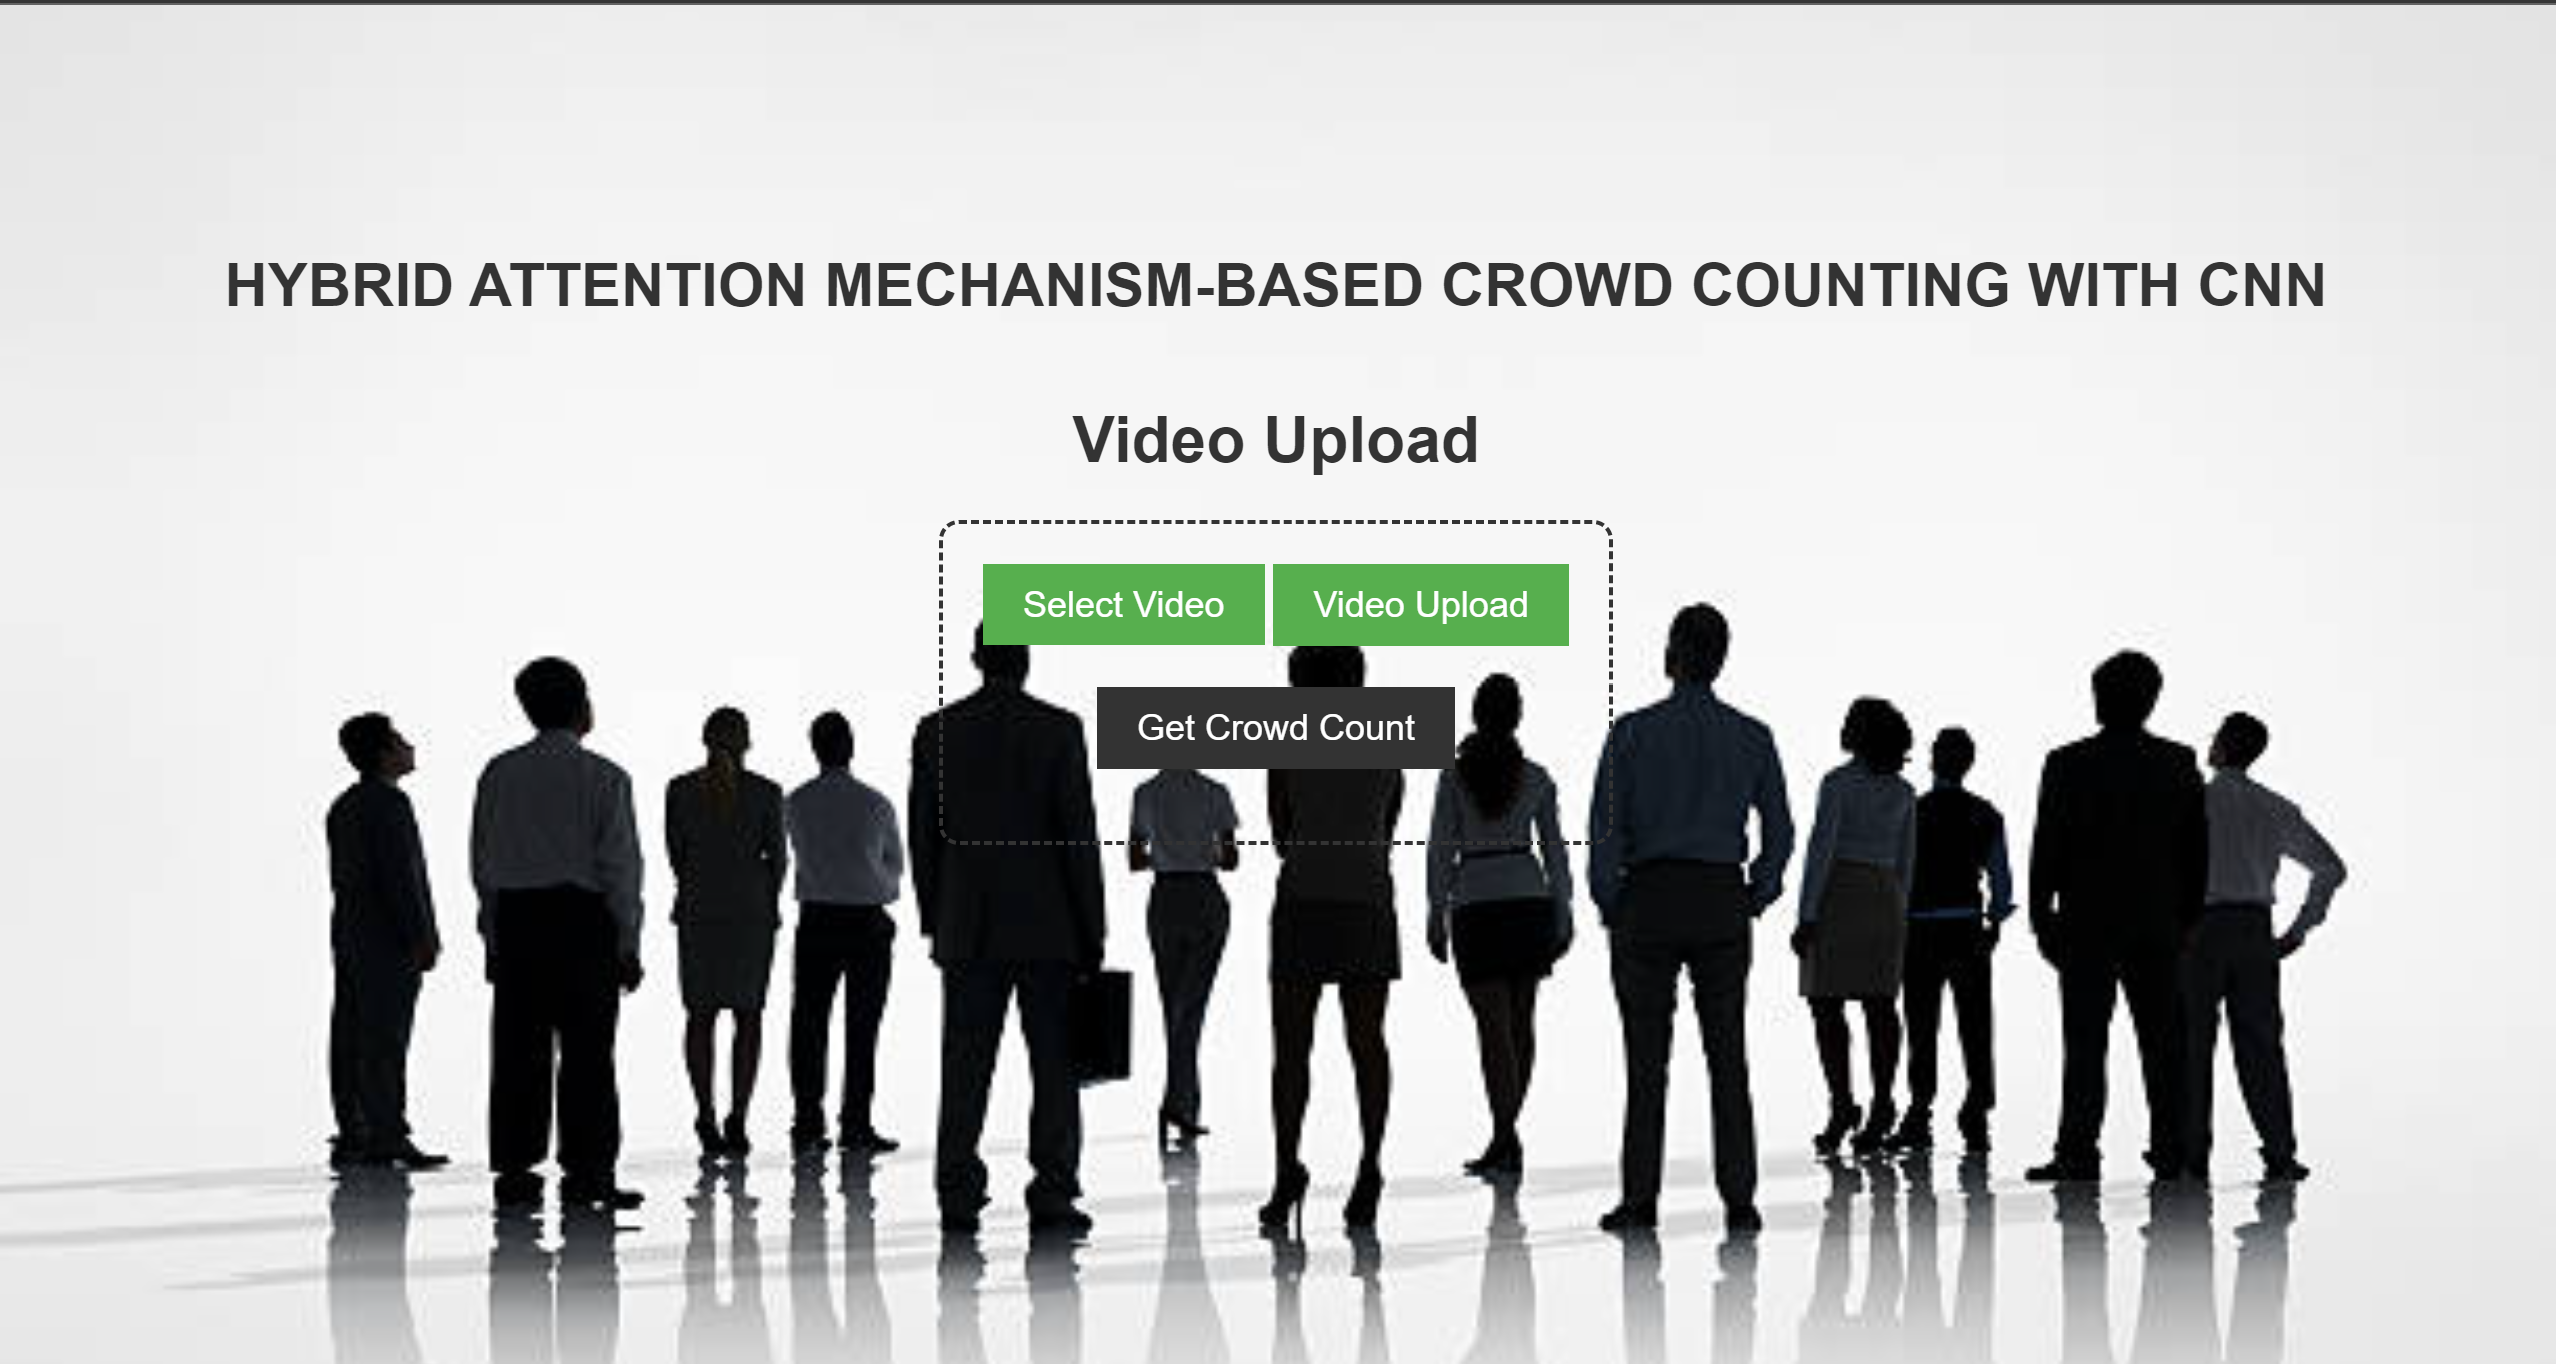
\includegraphics [width=0.9\textwidth, height=8cm]{1.png}
  \caption{Output UI 1}
  \label{fig:image}
\end{figure}

\begin{figure}[htbp]
  \centering
  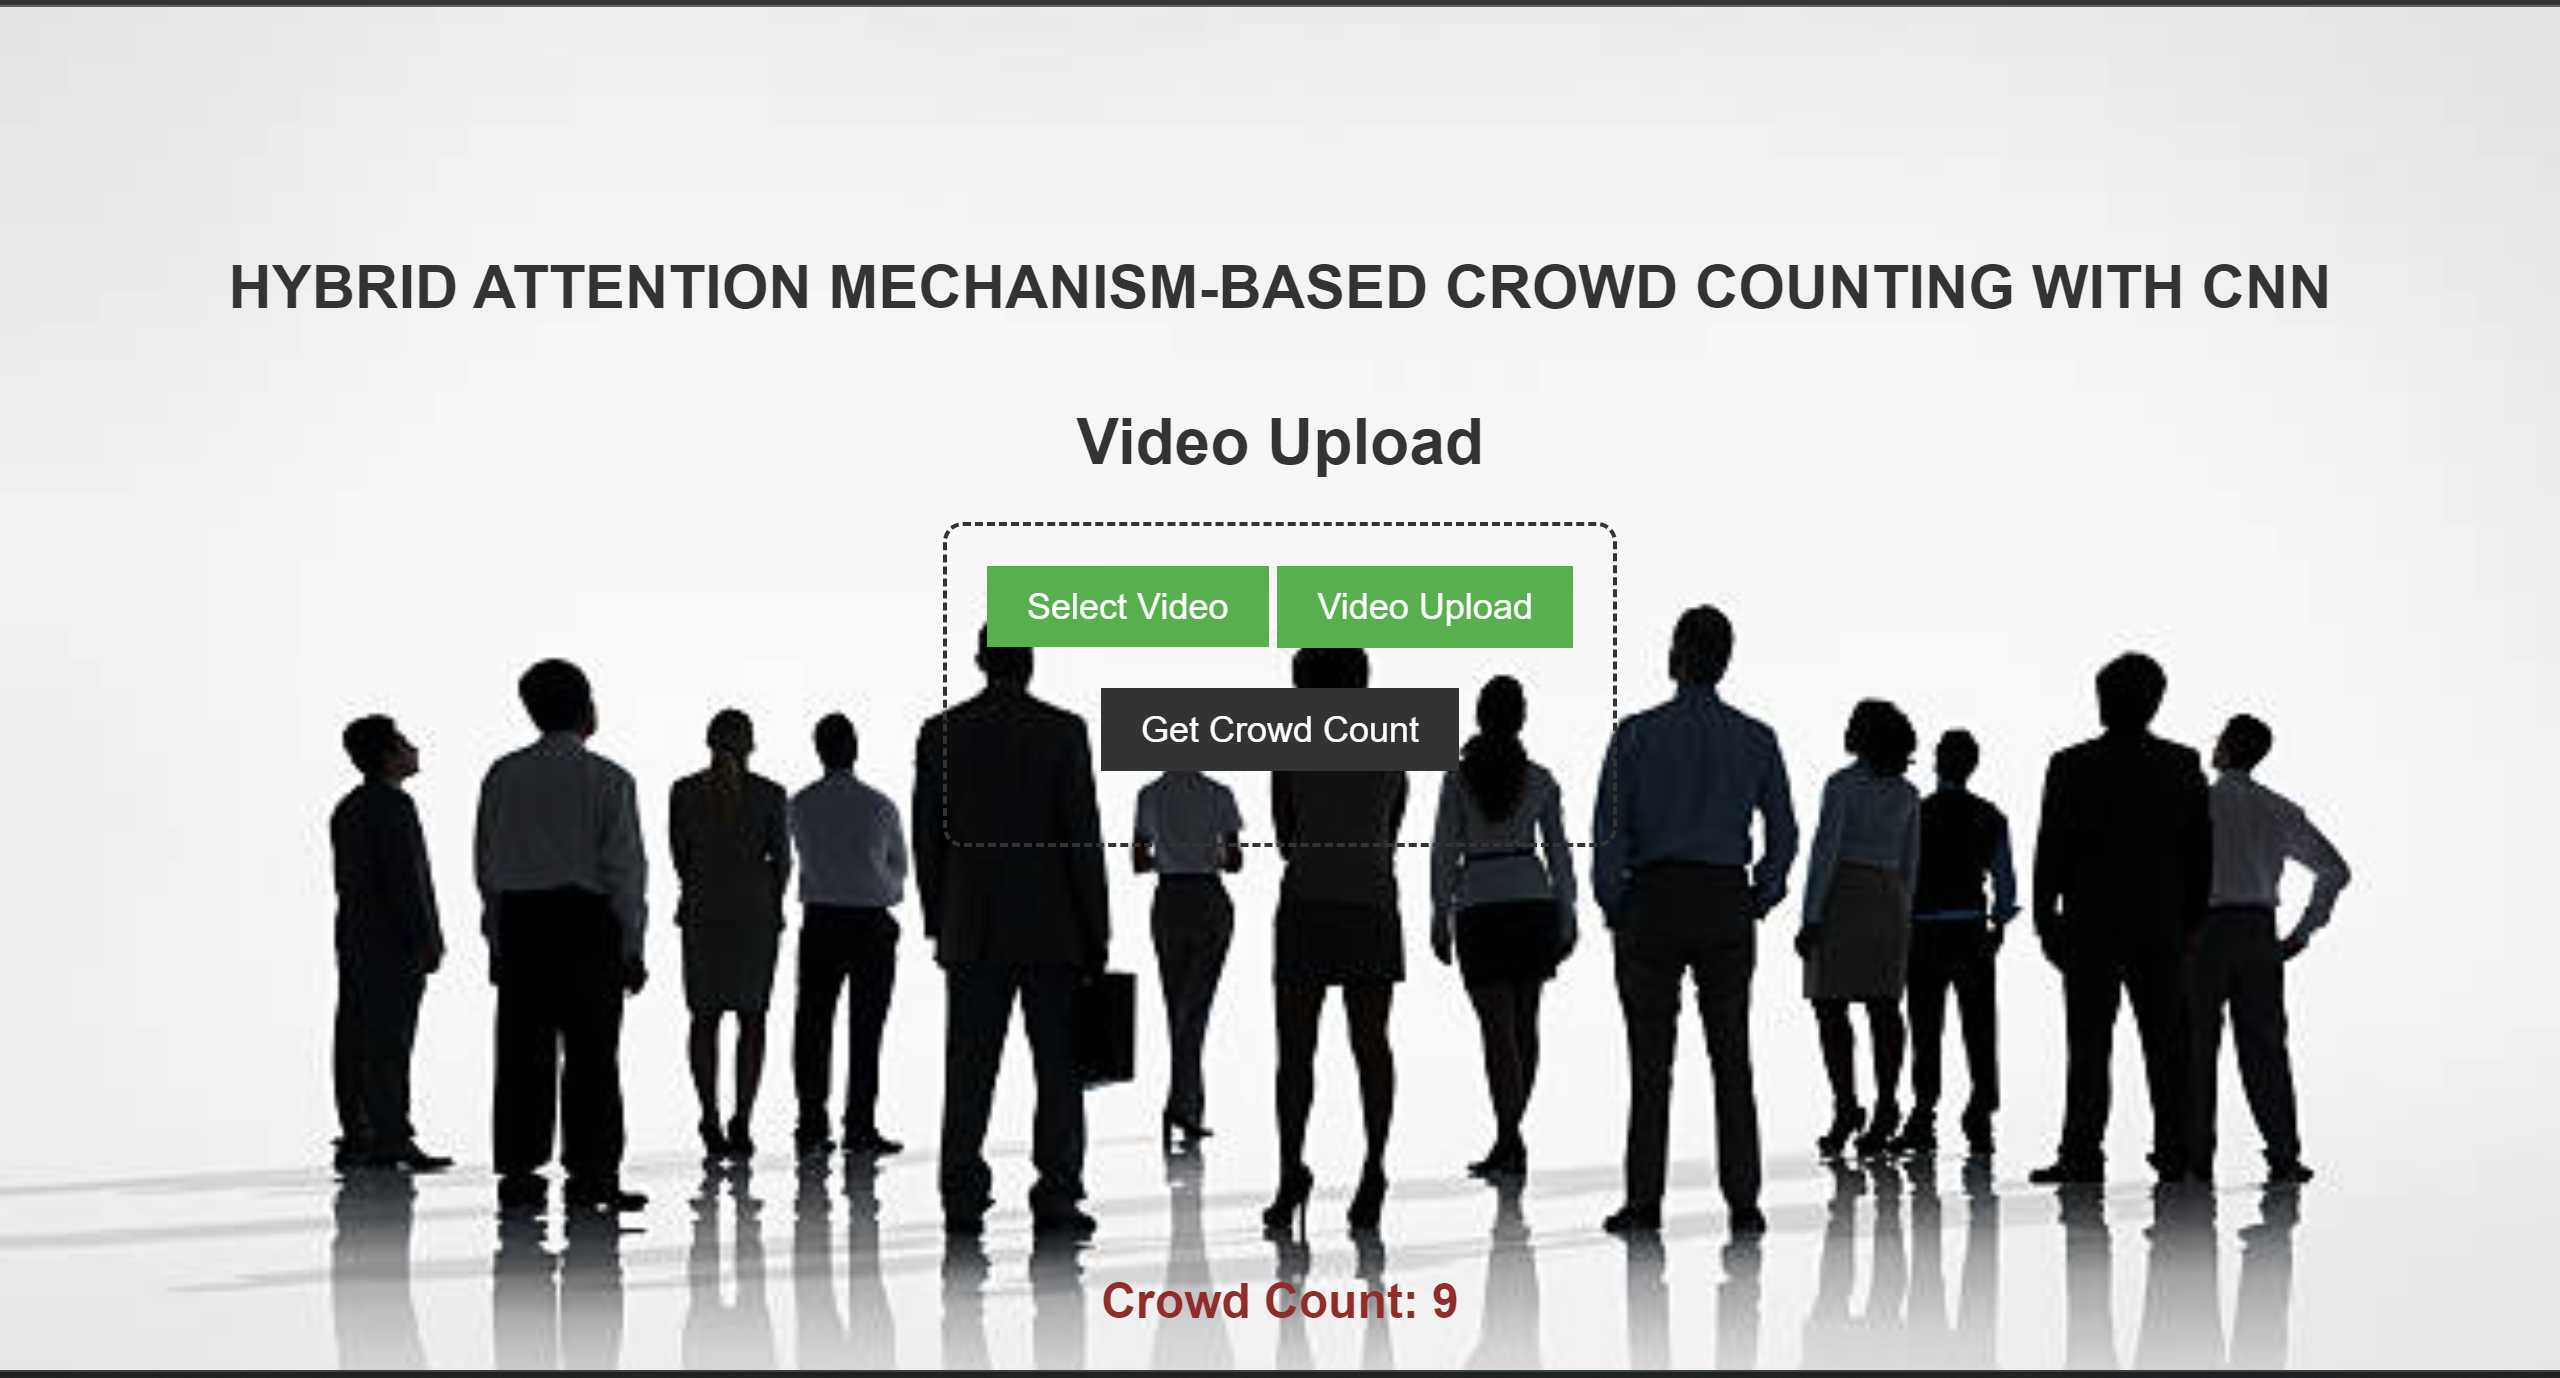
\includegraphics [width=0.9\textwidth, height=8cm]{2.png}
  \caption{Output UI 2}
  \label{fig:image}
\end{figure}

\begin{figure}[htbp]
  \centering
  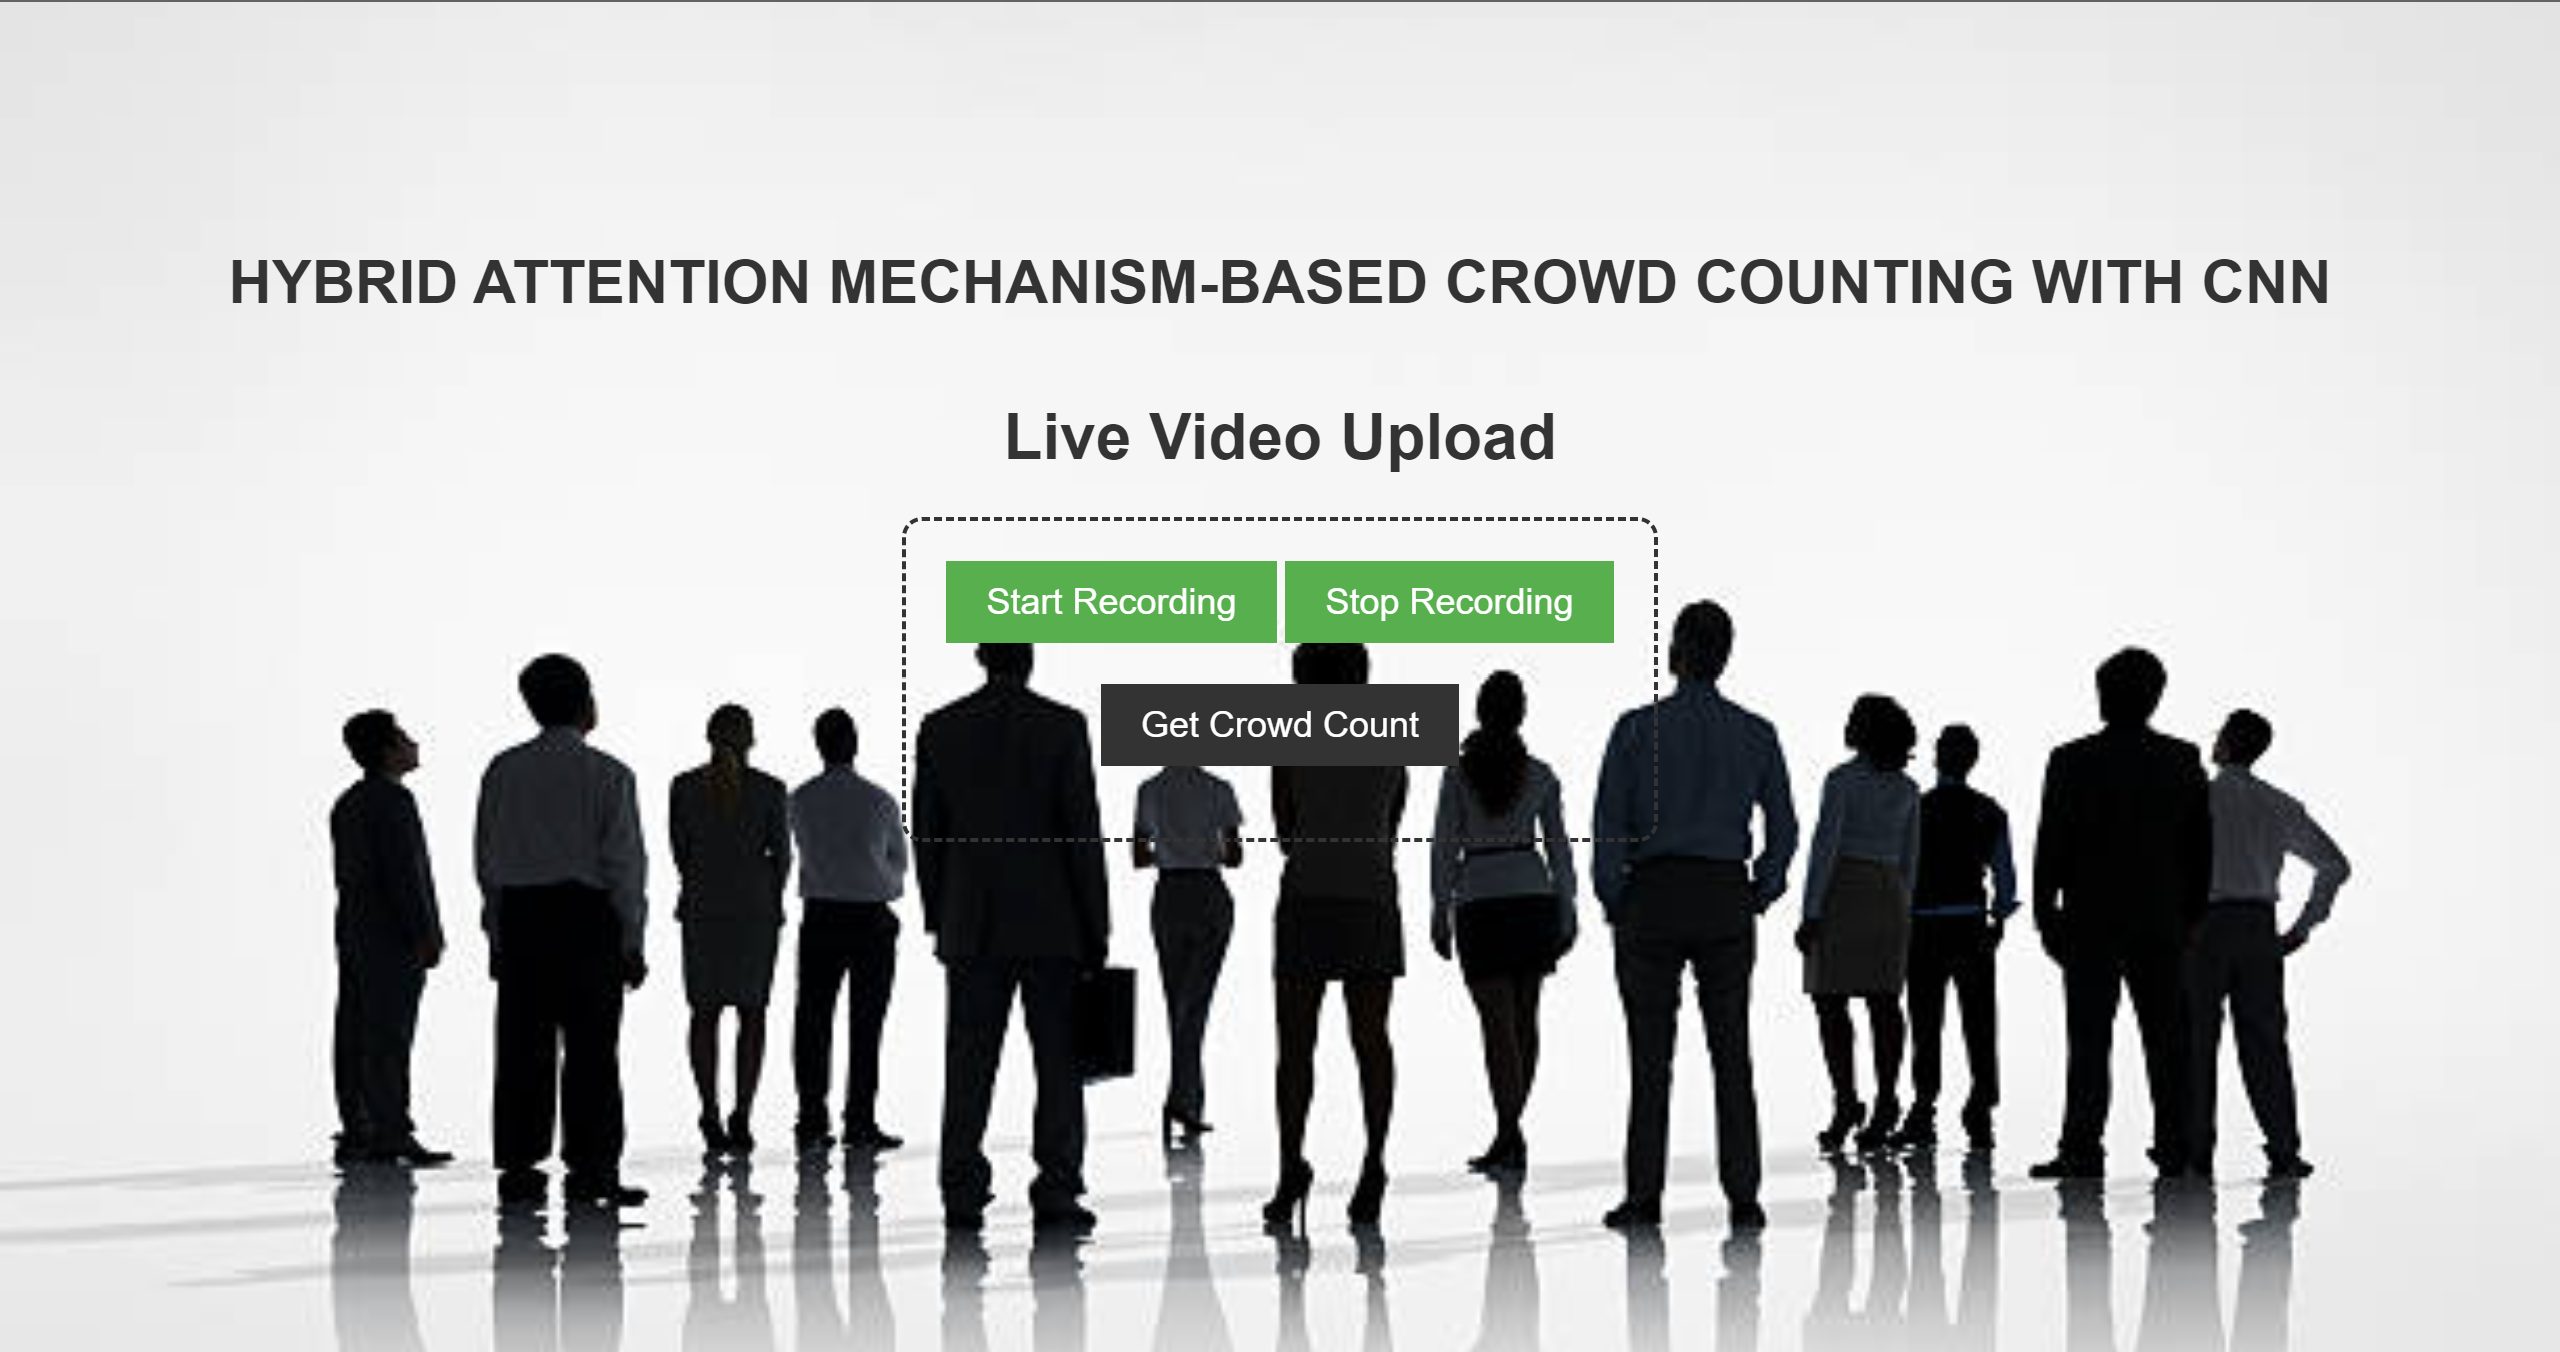
\includegraphics [width=0.9\textwidth, height=8cm]{3.png}
  \caption{Output UI 3}
  \label{fig:image}
\end{figure}

\begin{figure}[htbp]
  \centering
  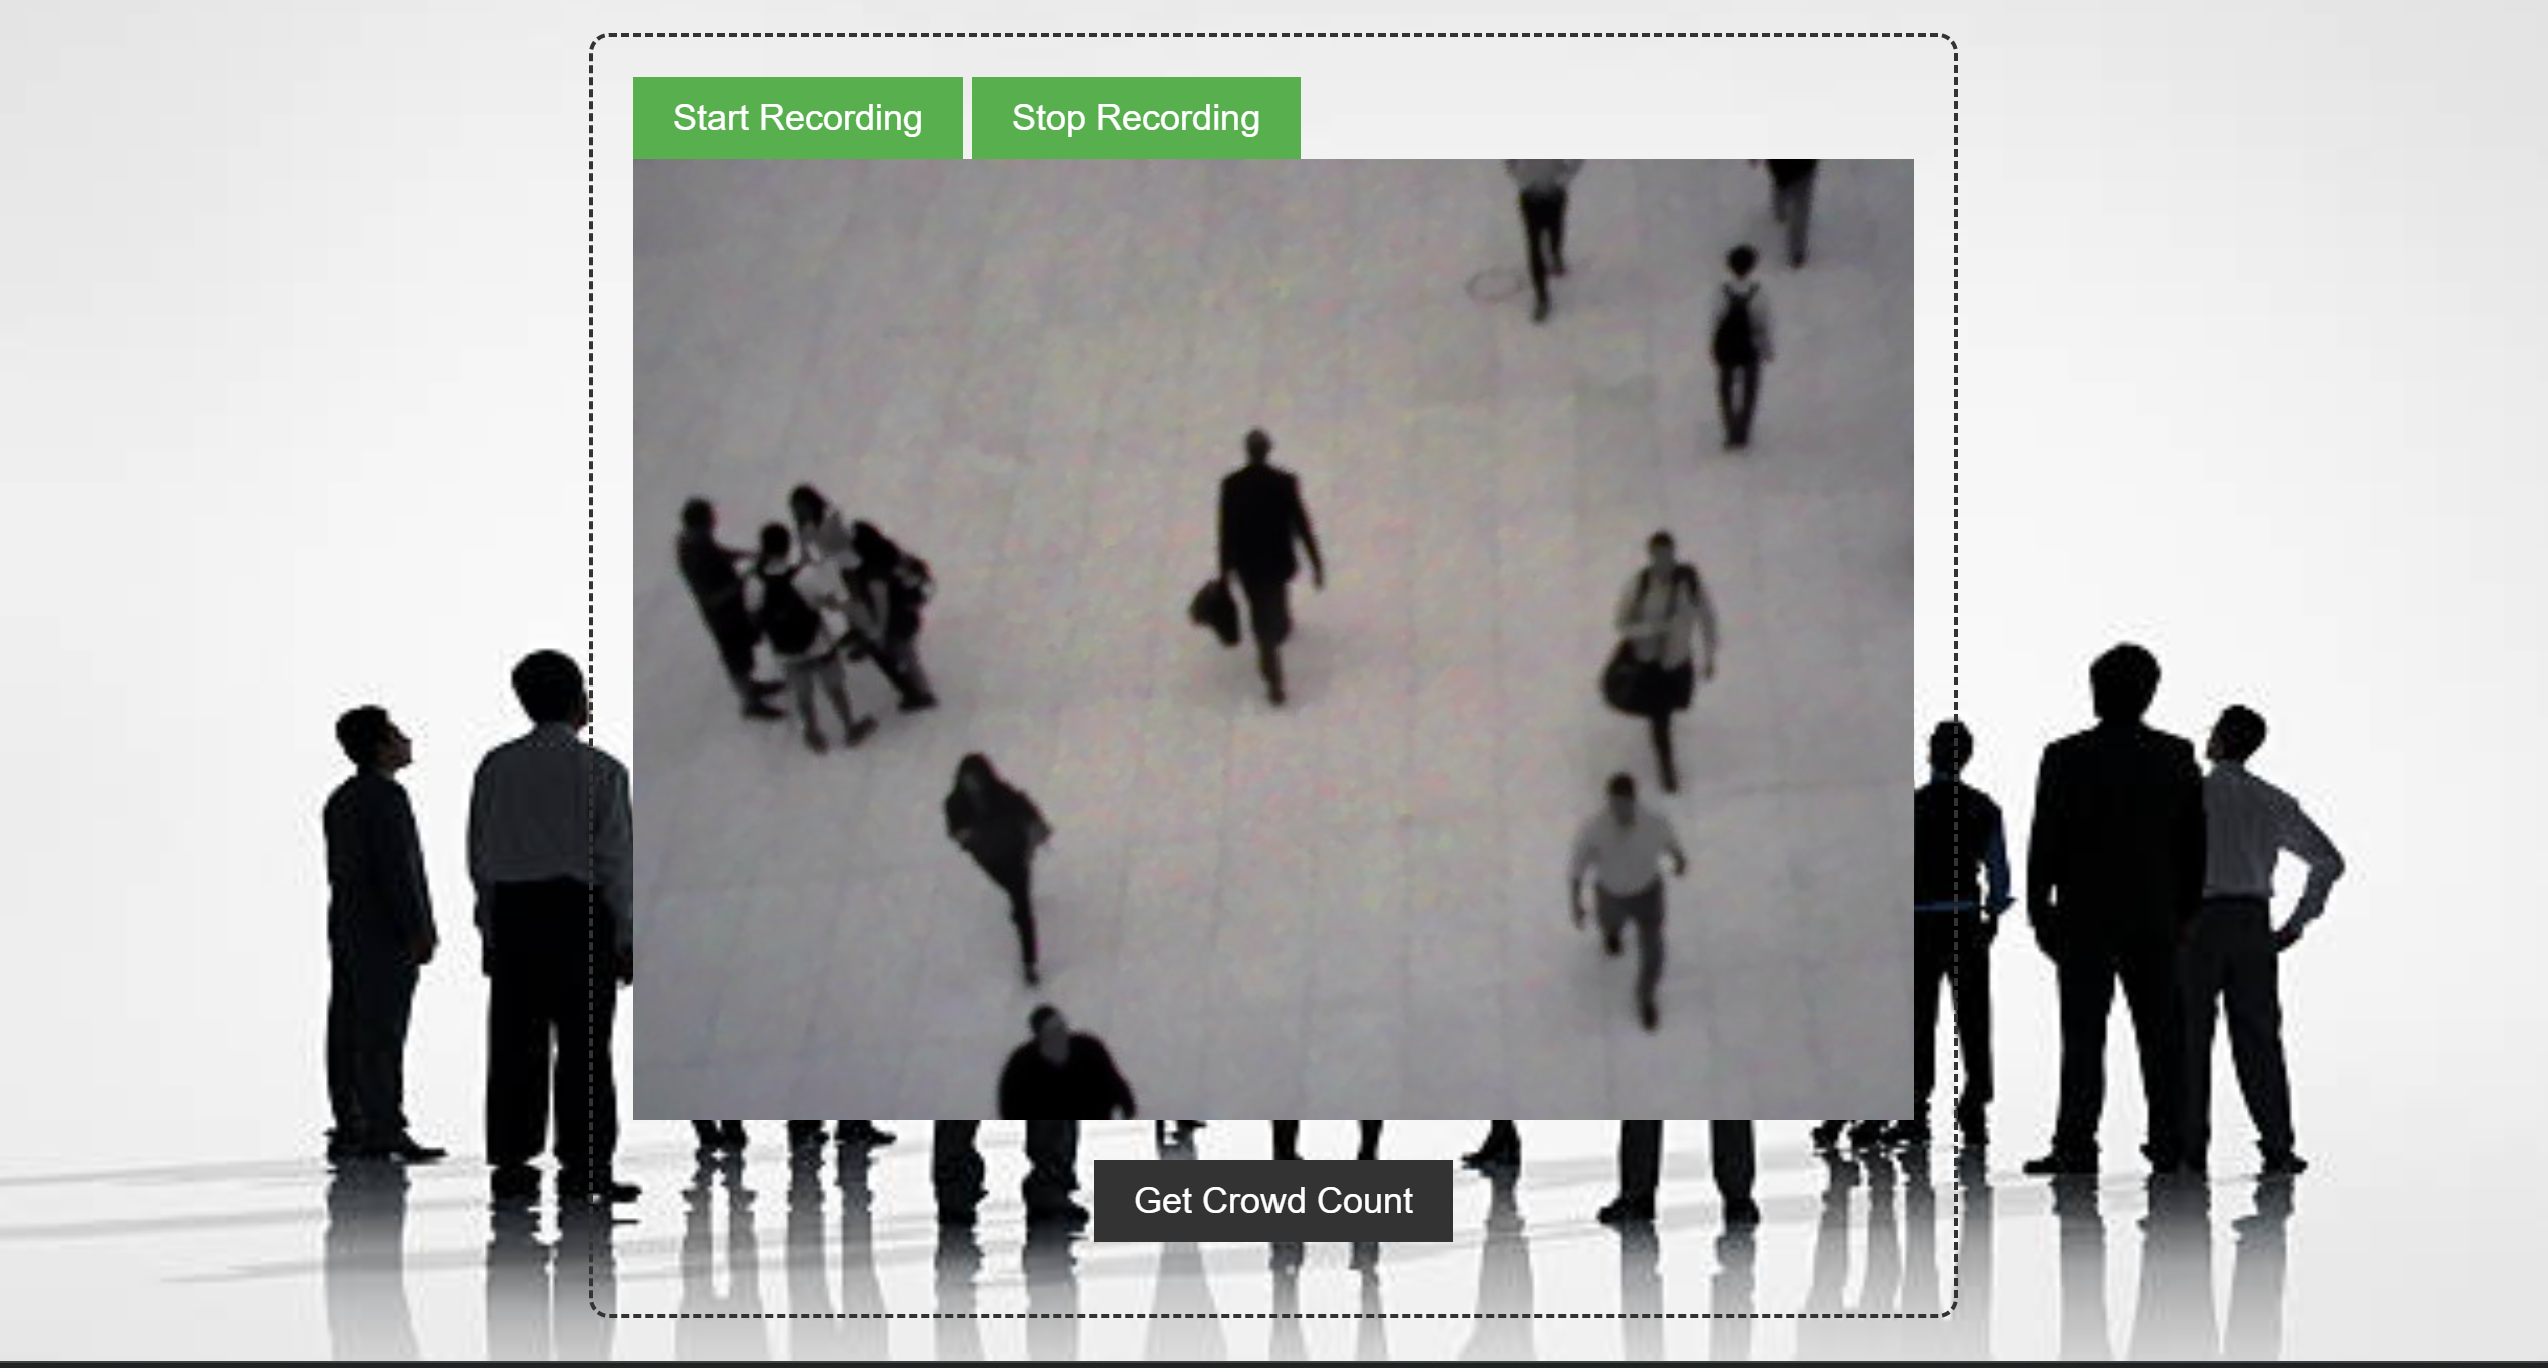
\includegraphics [width=0.9\textwidth, height=8cm]{4.png}
  \caption{Output UI 4}
  \label{fig:image}
\end{figure}

\begin{figure}[htbp]
  \centering
  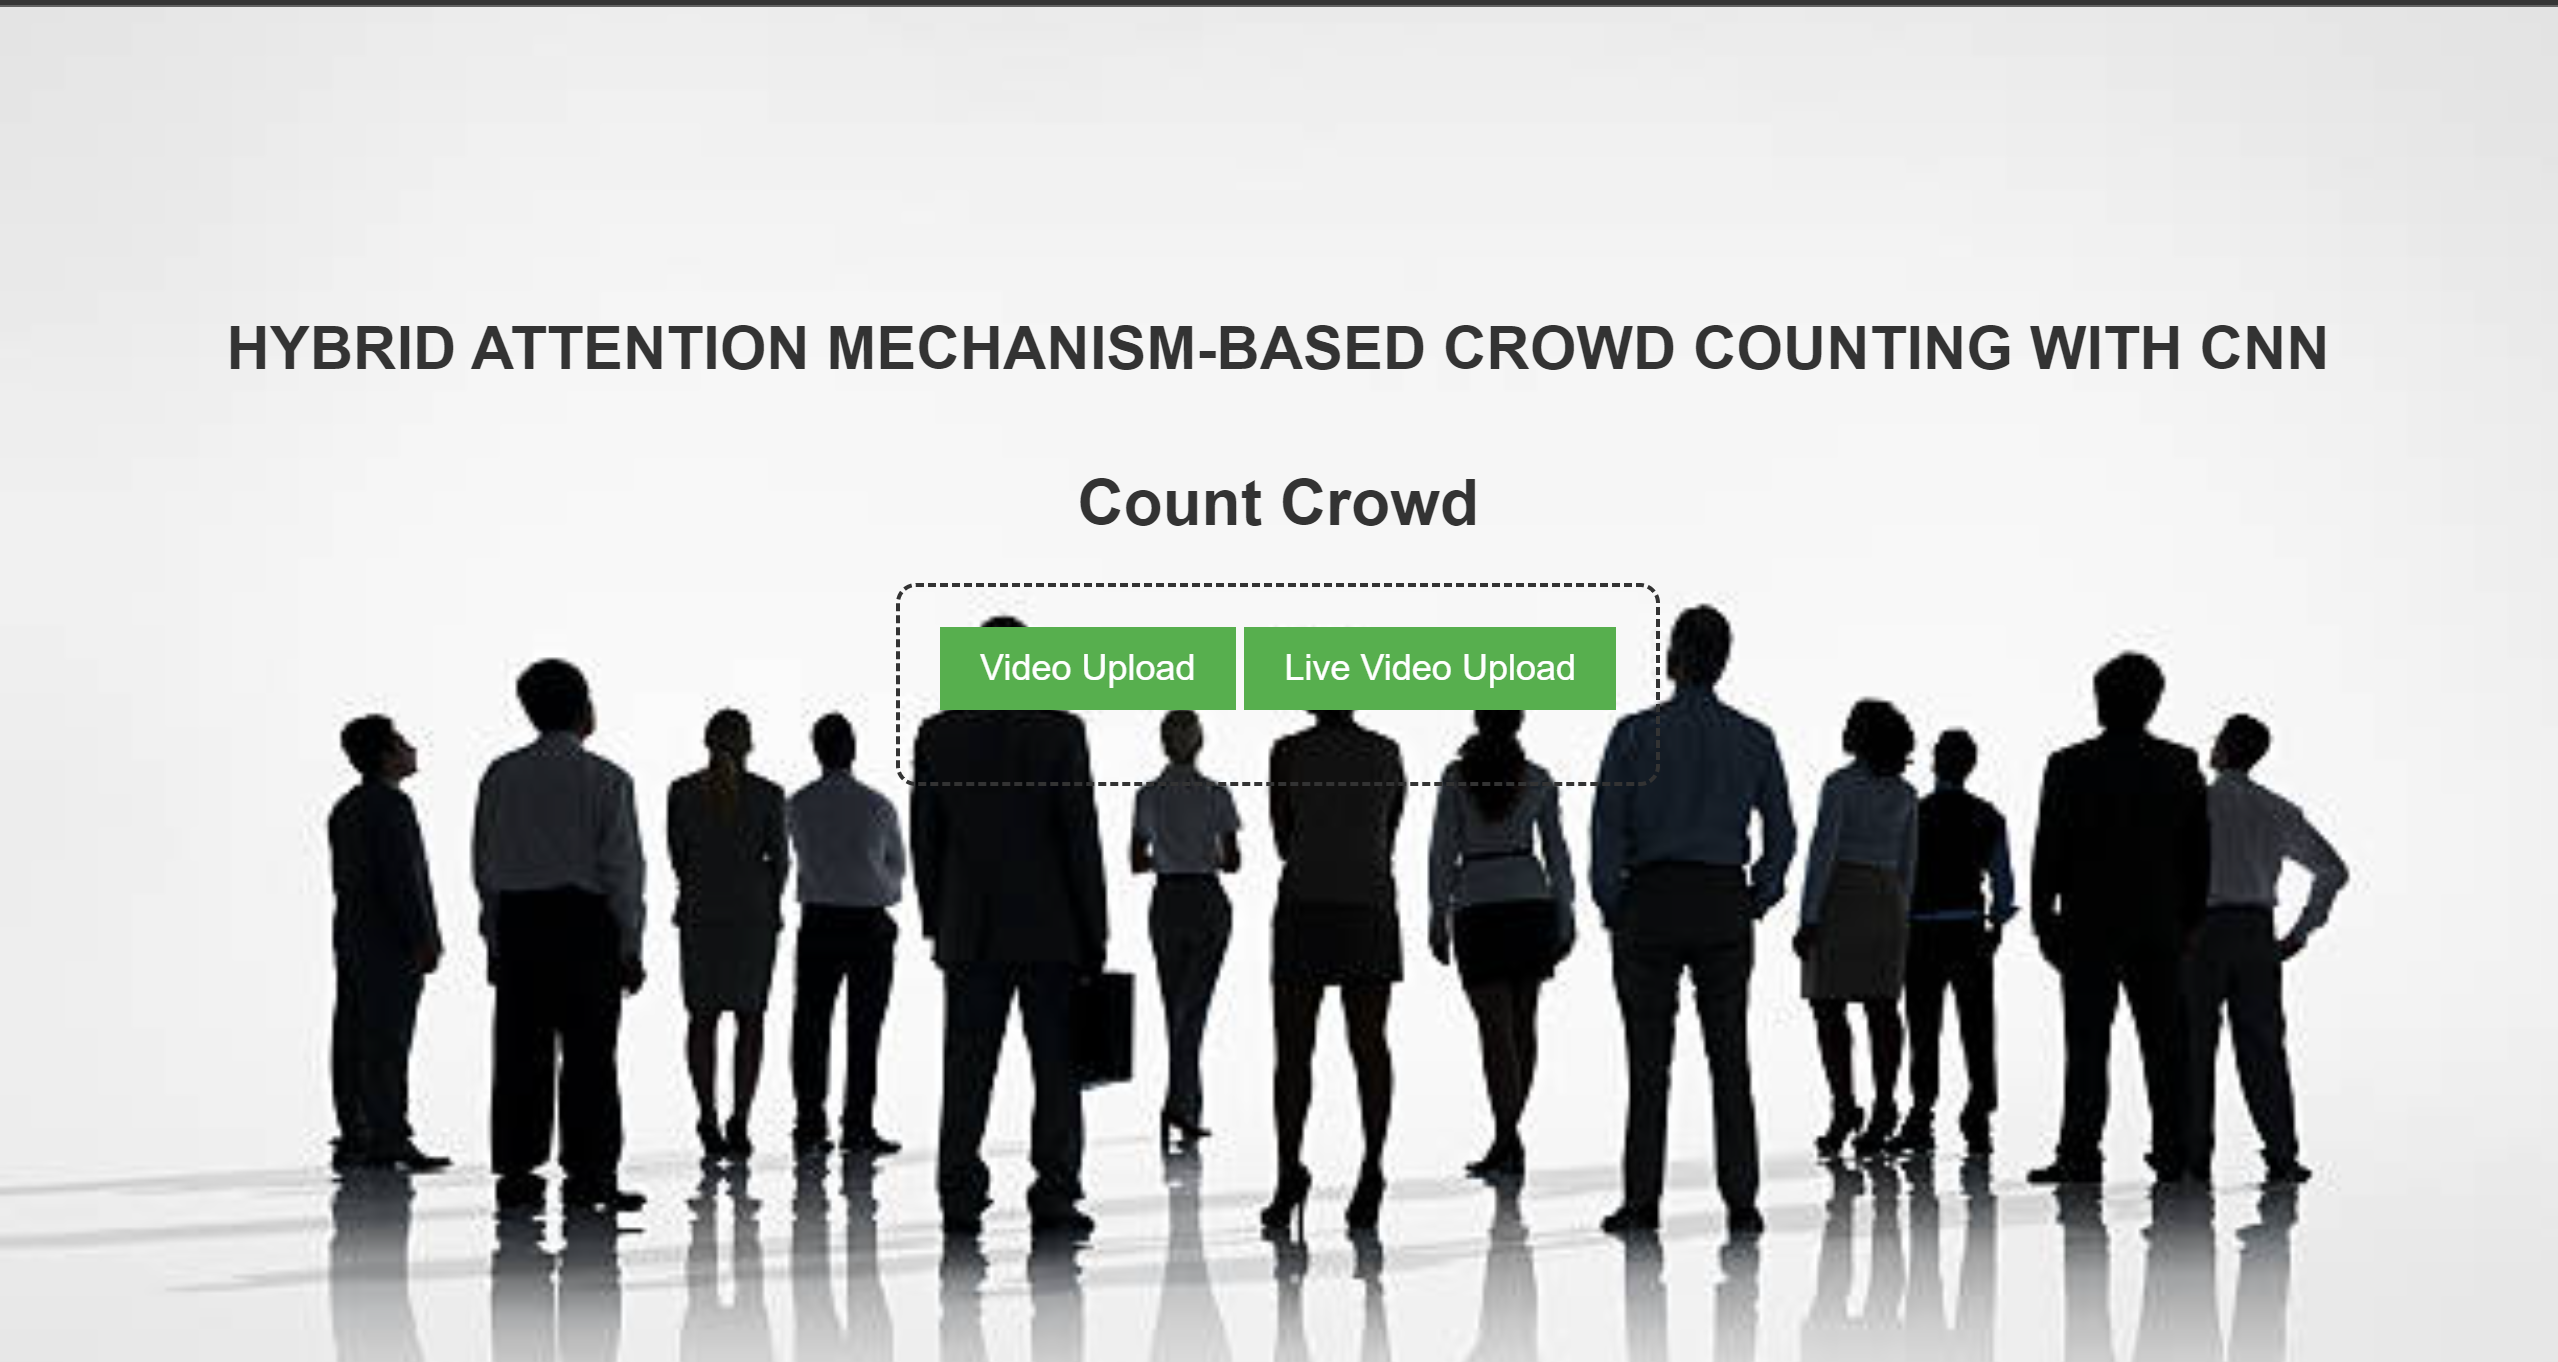
\includegraphics [width=0.9\textwidth, height=8cm]{5.png}
  \caption{Output UI 5}
  \label{fig:image}
\end{figure}

\begin{figure}[htbp]
  \centering
  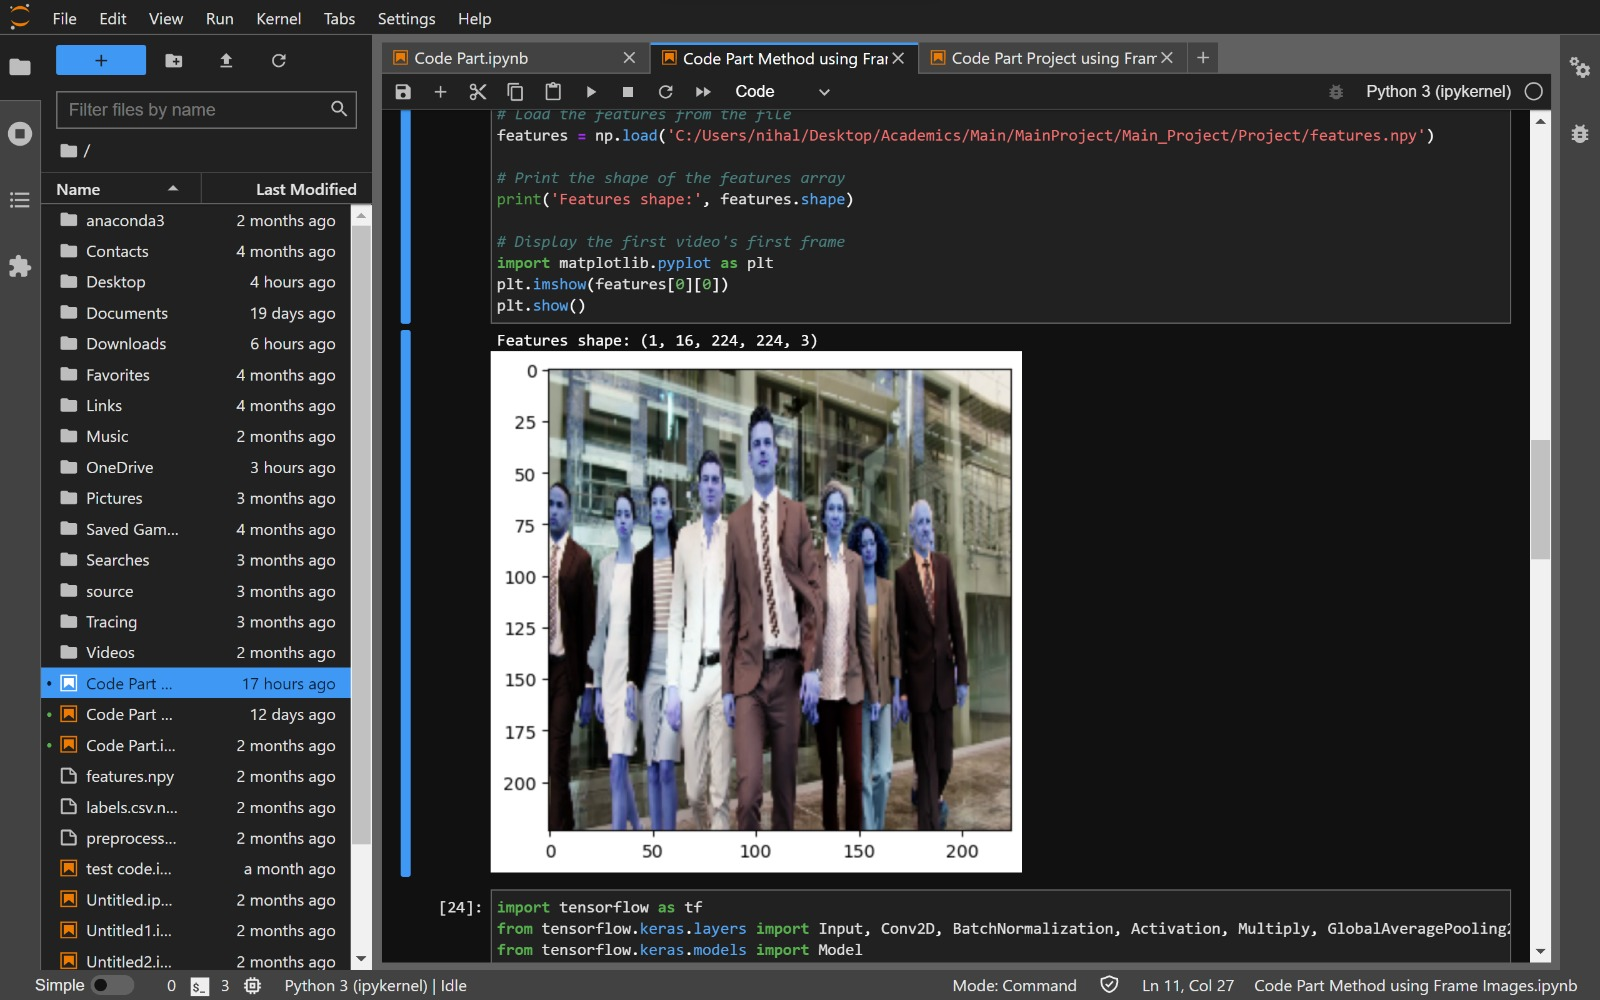
\includegraphics [width=0.9\textwidth, height=8cm]{6.jpeg}
  \caption{Output 1}
  \label{fig:image}
\end{figure}

\begin{figure}[htbp]
  \centering
  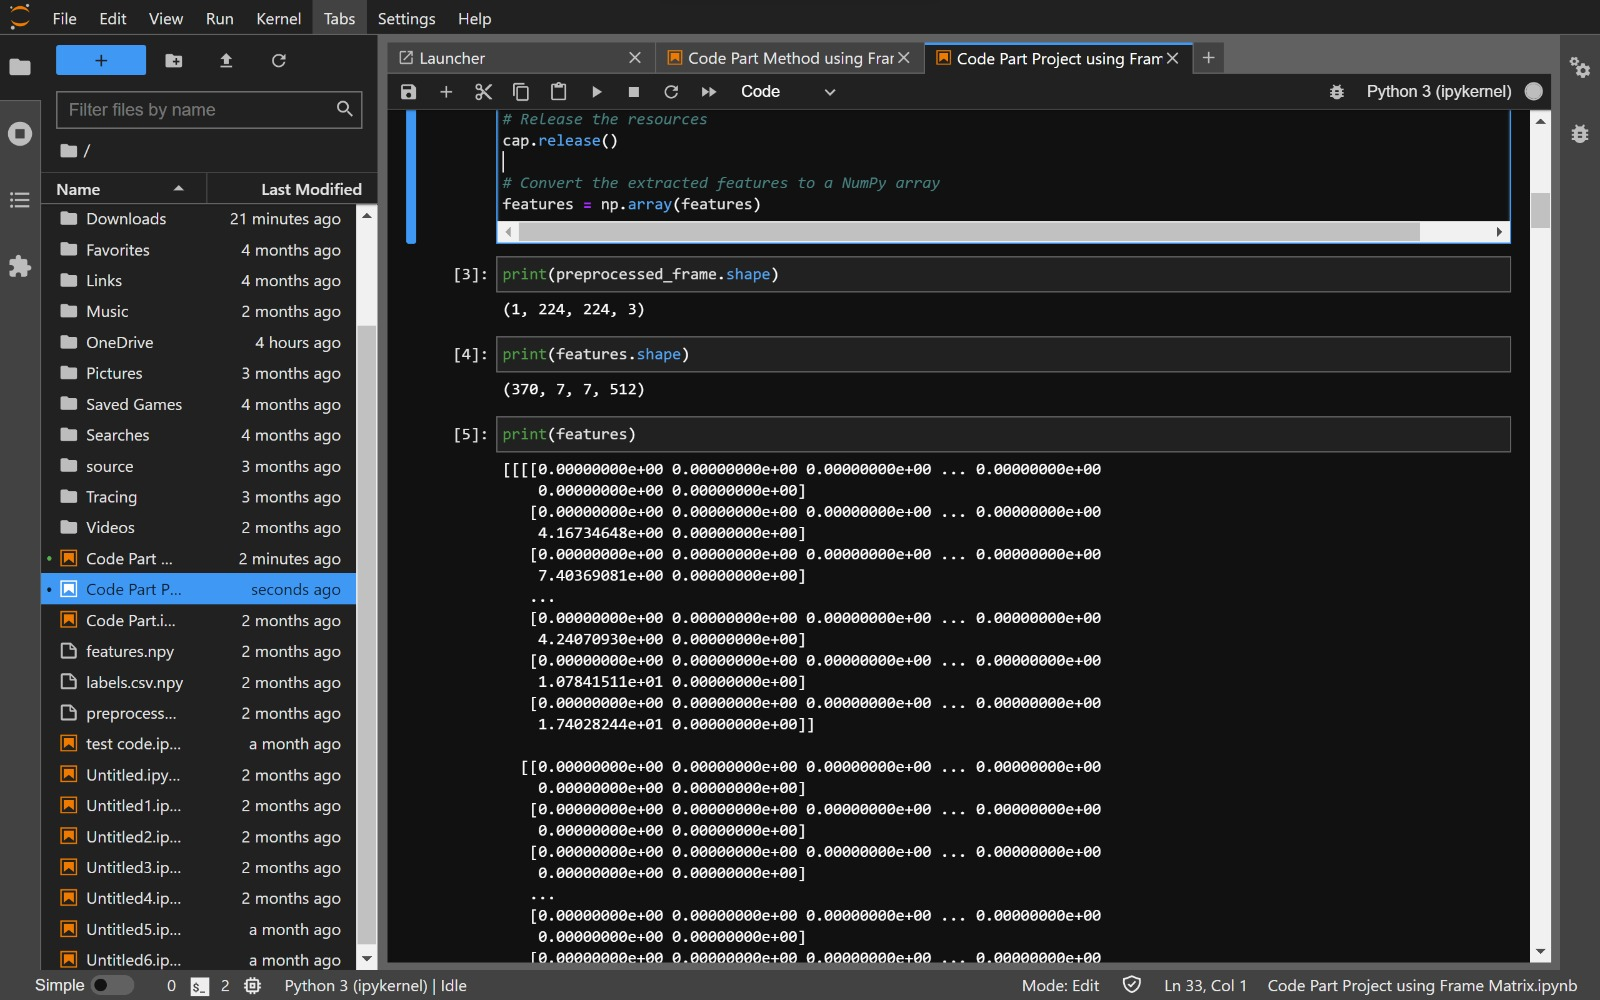
\includegraphics [width=0.9\textwidth, height=8cm]{7.jpeg}
  \caption{Output 2}
  \label{fig:image}
\end{figure}

\begin{figure}[htbp]
  \centering
  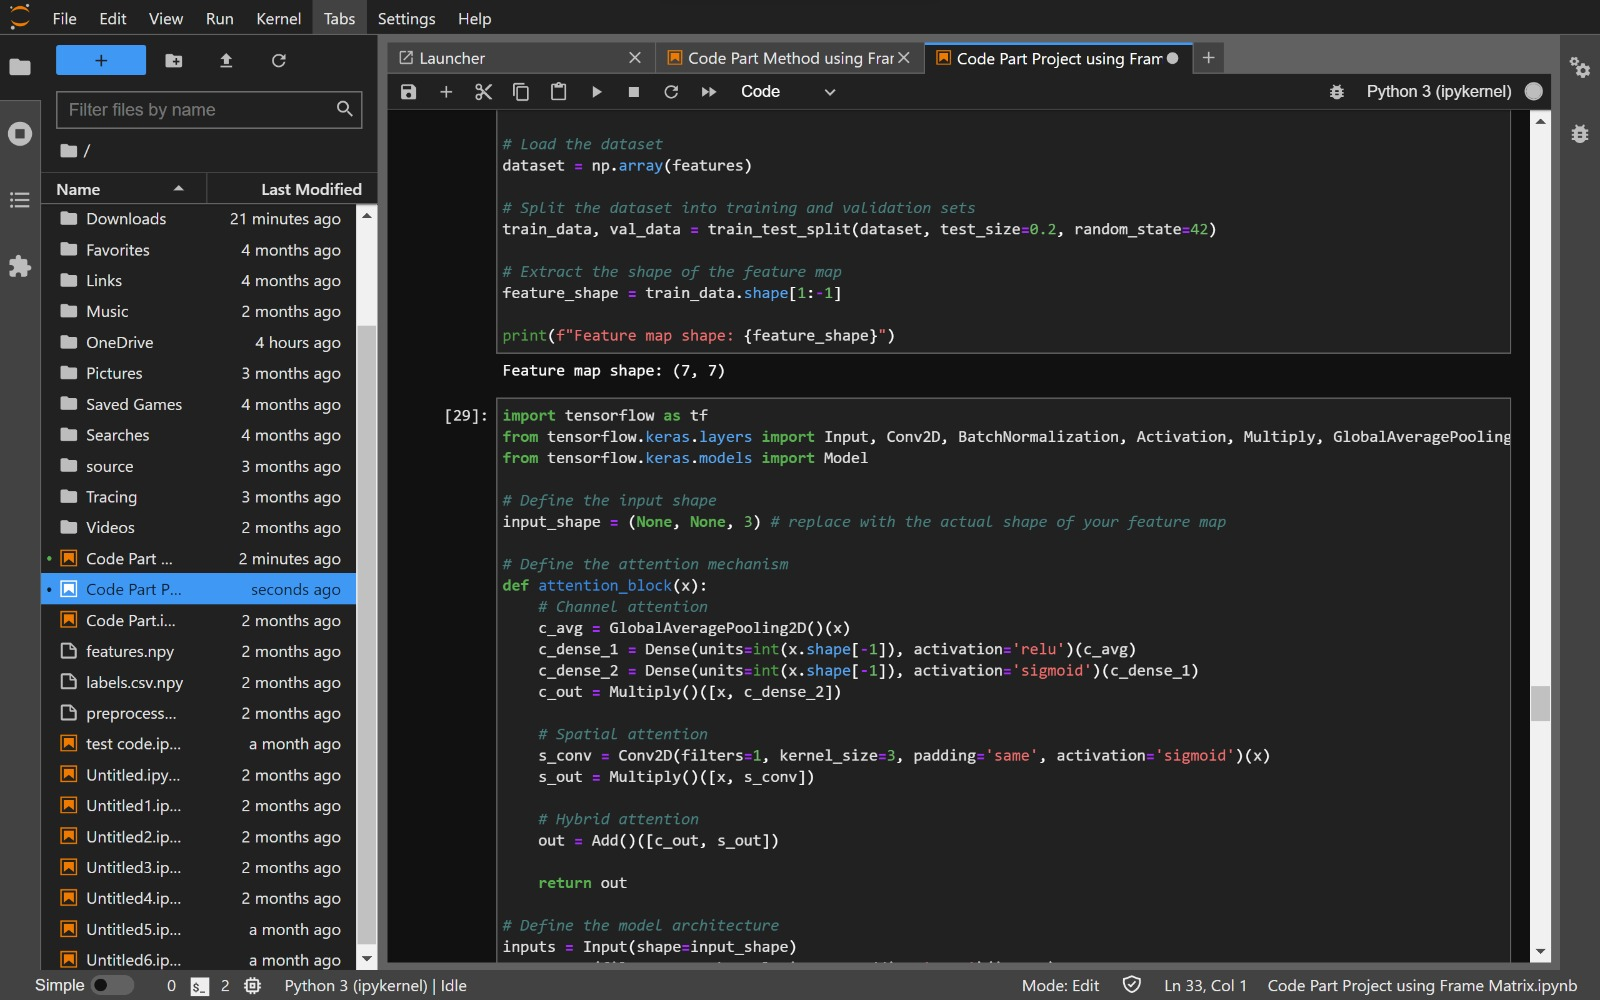
\includegraphics [width=0.9\textwidth, height=8cm]{8.jpeg}
  \caption{Output 3}
  \label{fig:image}
\end{figure}

\begin{figure}[htbp]
  \centering
  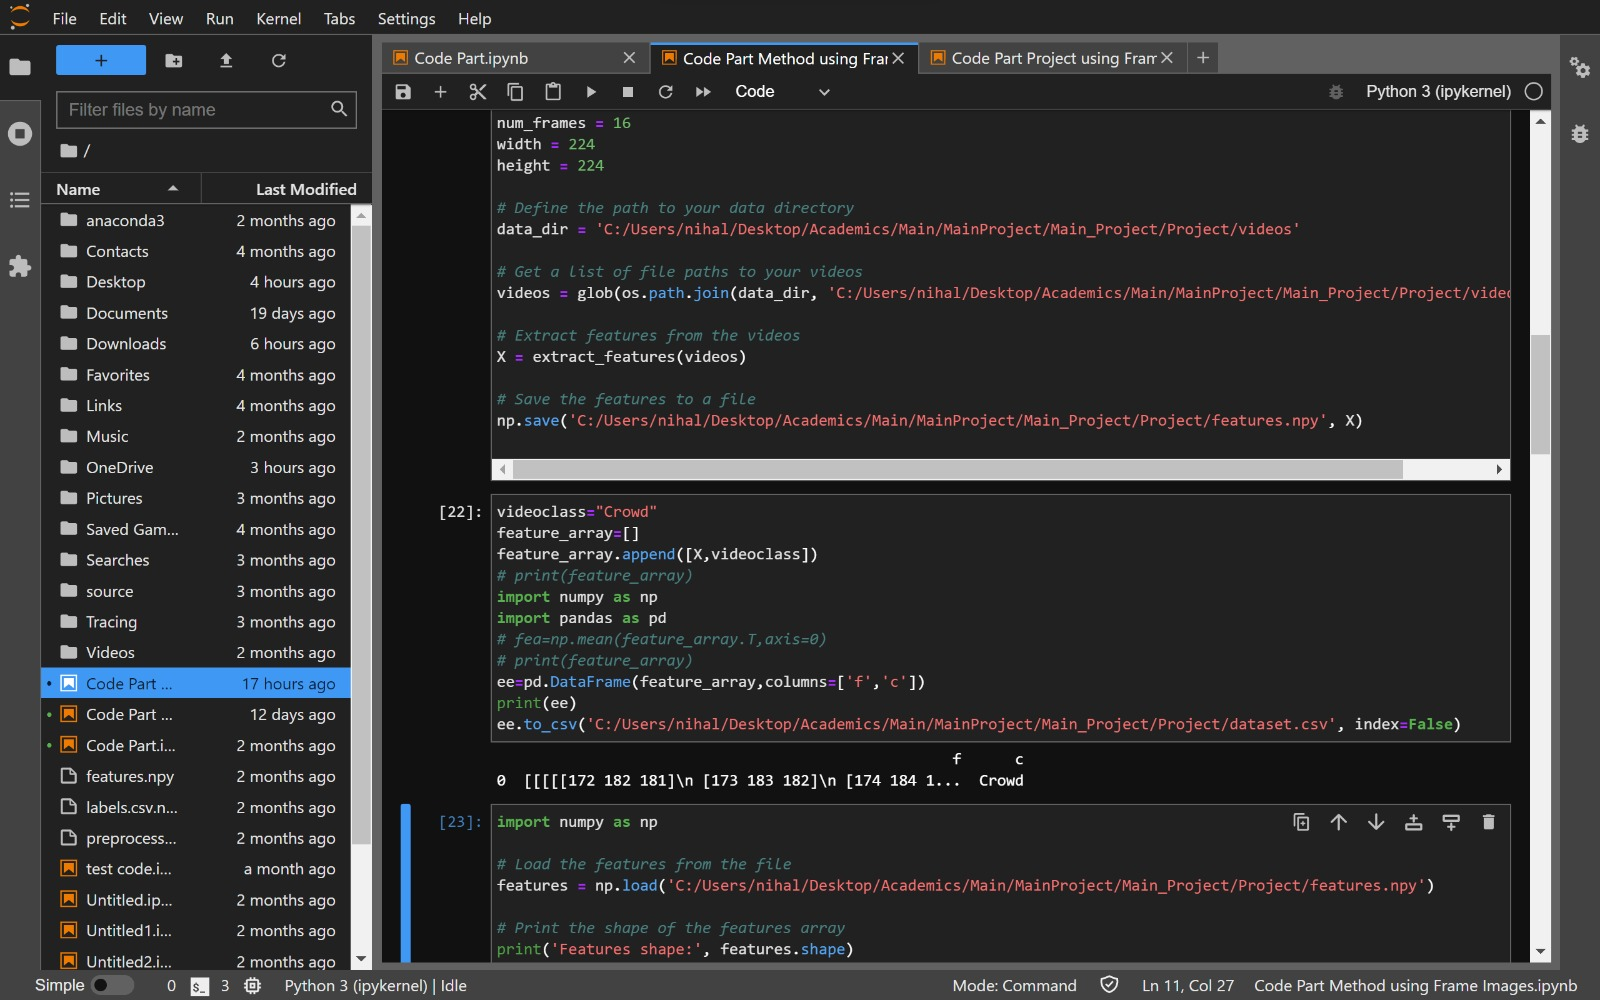
\includegraphics [width=0.9\textwidth, height=8cm]{9.jpeg}
  \caption{Output 4}
  \label{fig:image}
\end{figure}

\begin{figure}[htbp]
  \centering
  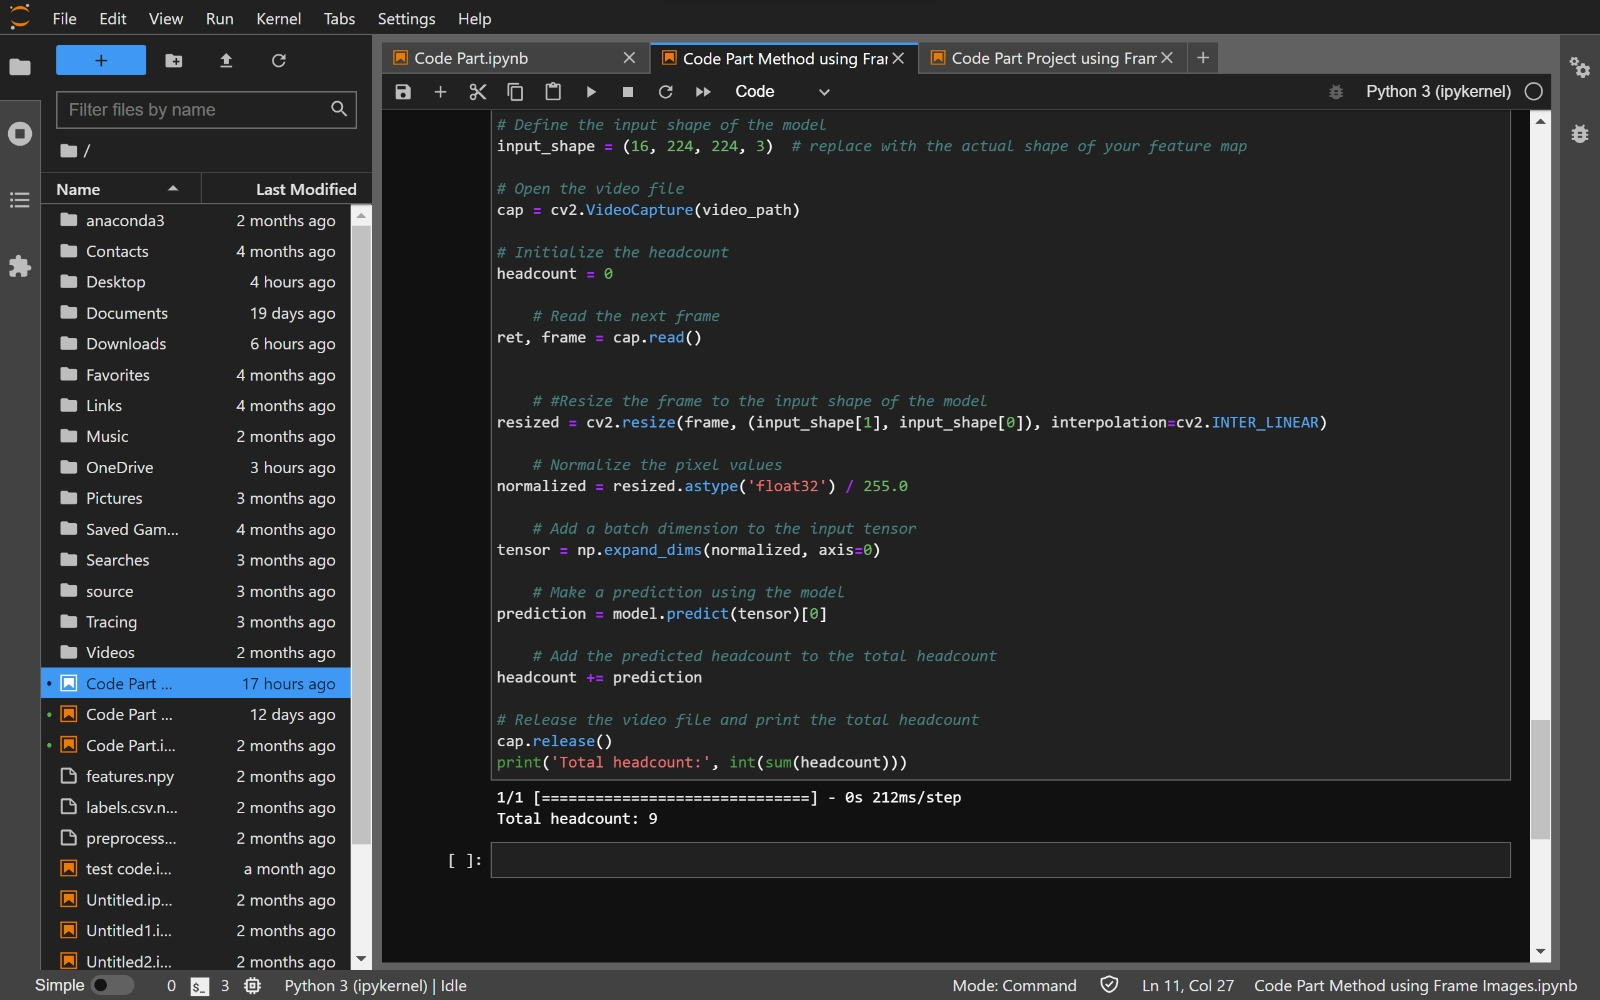
\includegraphics [width=0.9\textwidth, height=8cm]{10.jpeg}
  \caption{Output 5}
  \label{fig:image}
\end{figure}

\chapter{Git History}

\begin{figure}[htbp]
  \centering
  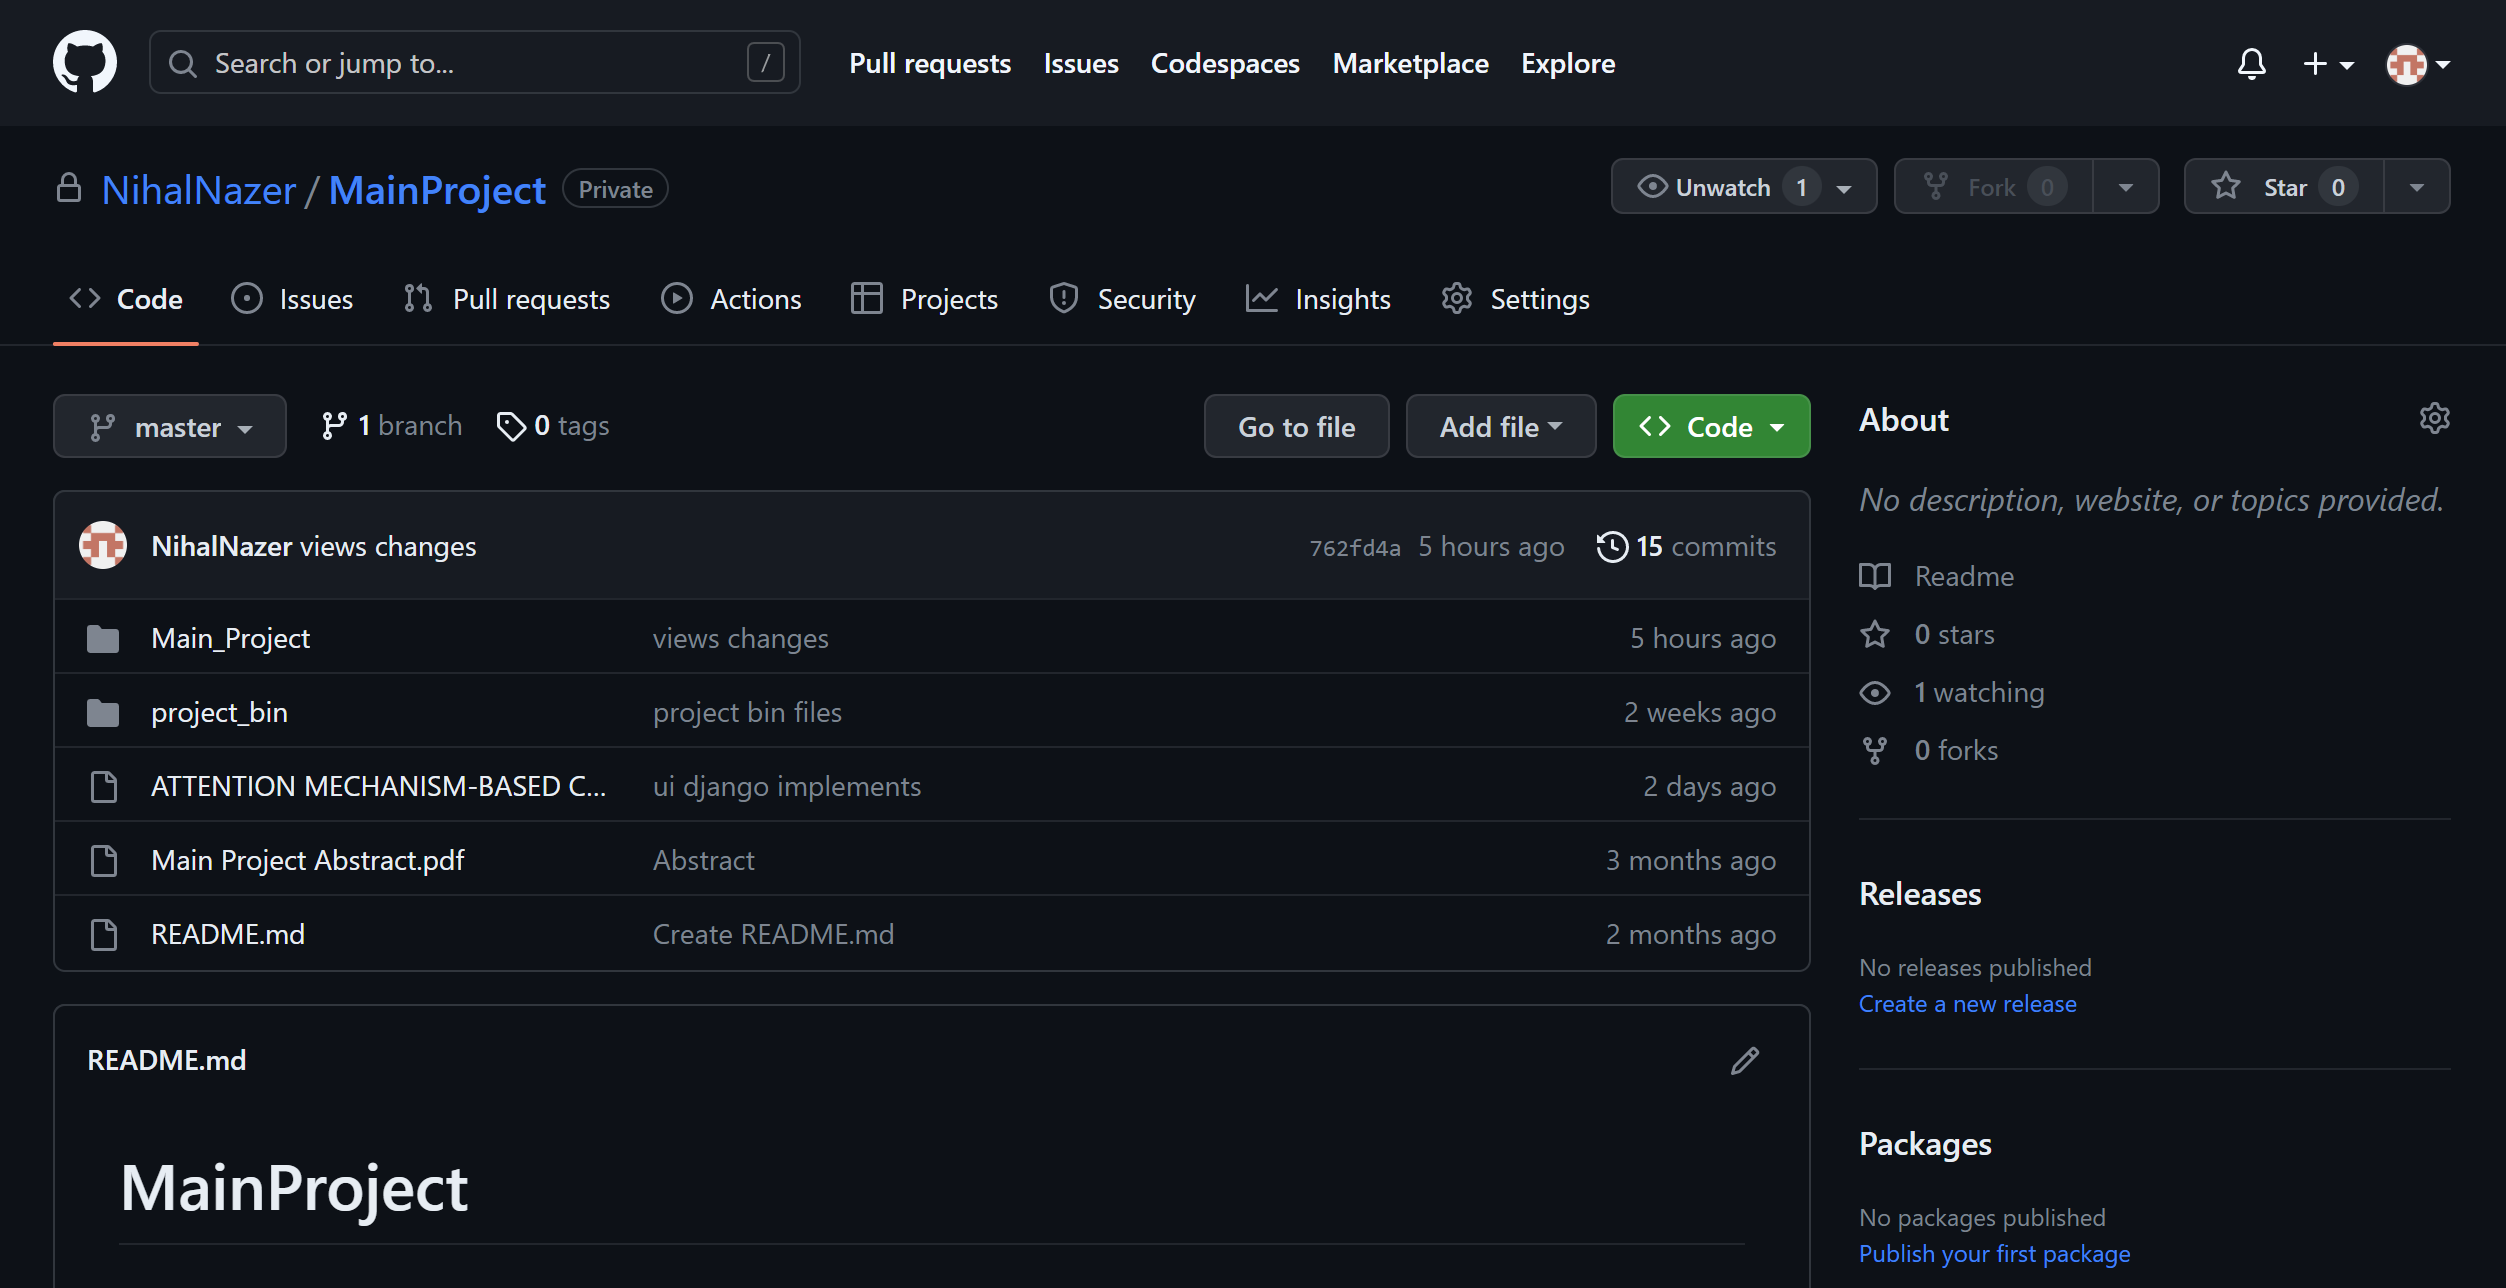
\includegraphics [width=0.9\textwidth, height=8cm]{git 1.png}
  \caption{Git 1}
  \label{fig:image}
\end{figure}

\begin{figure}[htbp]
  \centering
  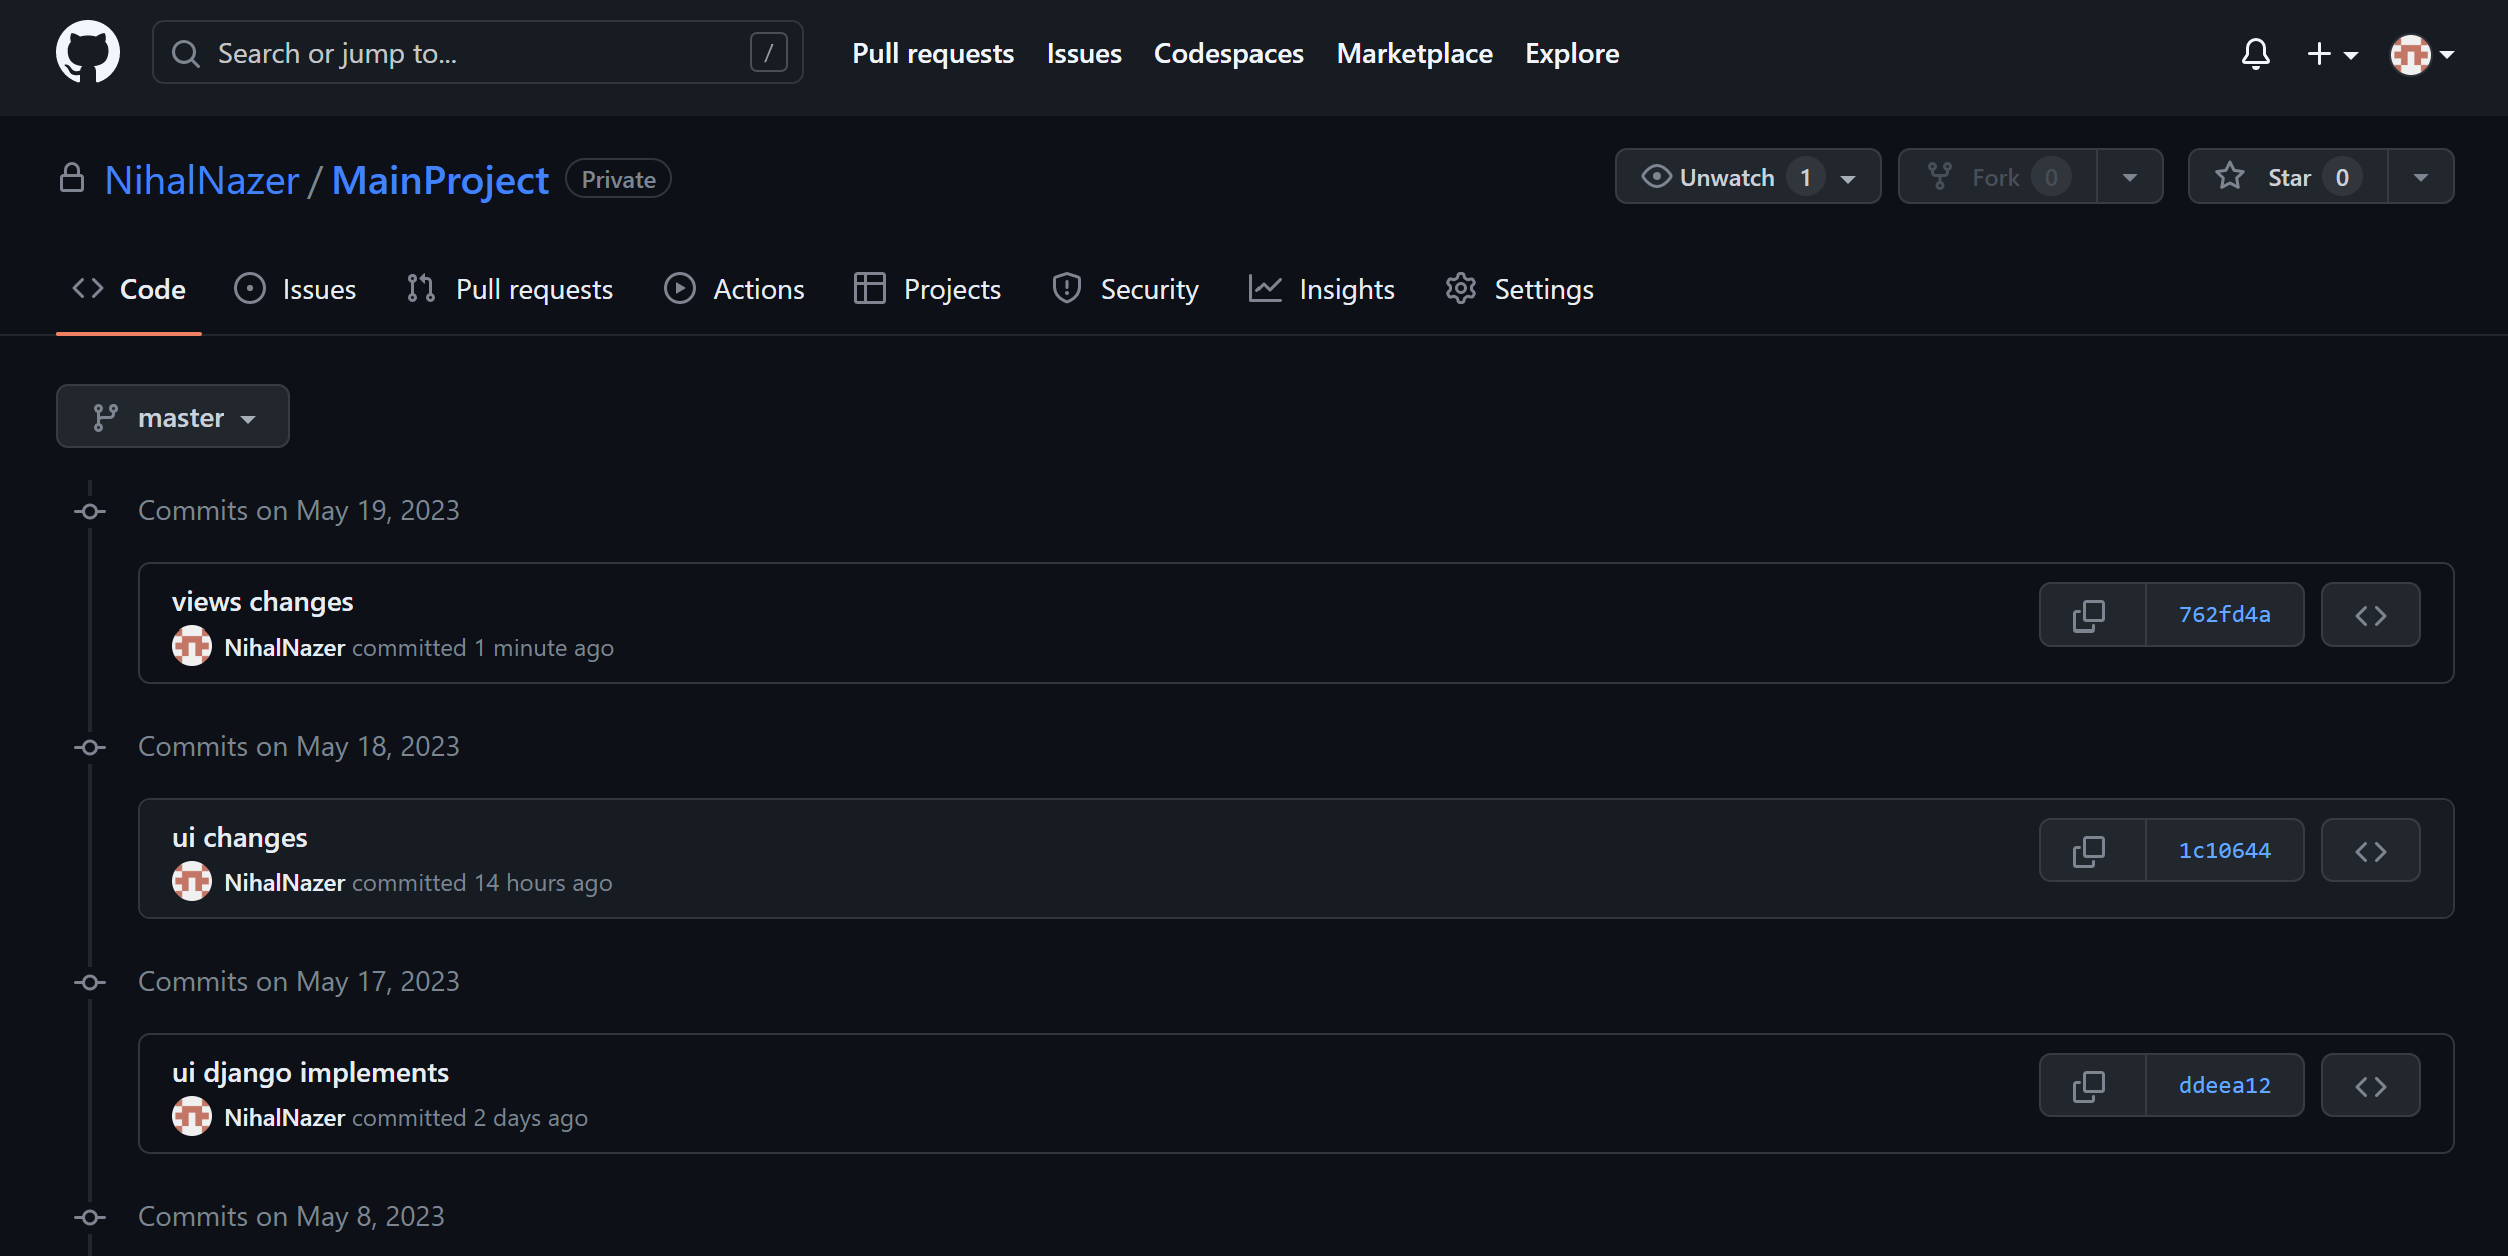
\includegraphics [width=0.9\textwidth, height=8cm]{git 2.png}
  \caption{Git 2}
  \label{fig:image}
\end{figure}

\begin{figure}[htbp]
  \centering
  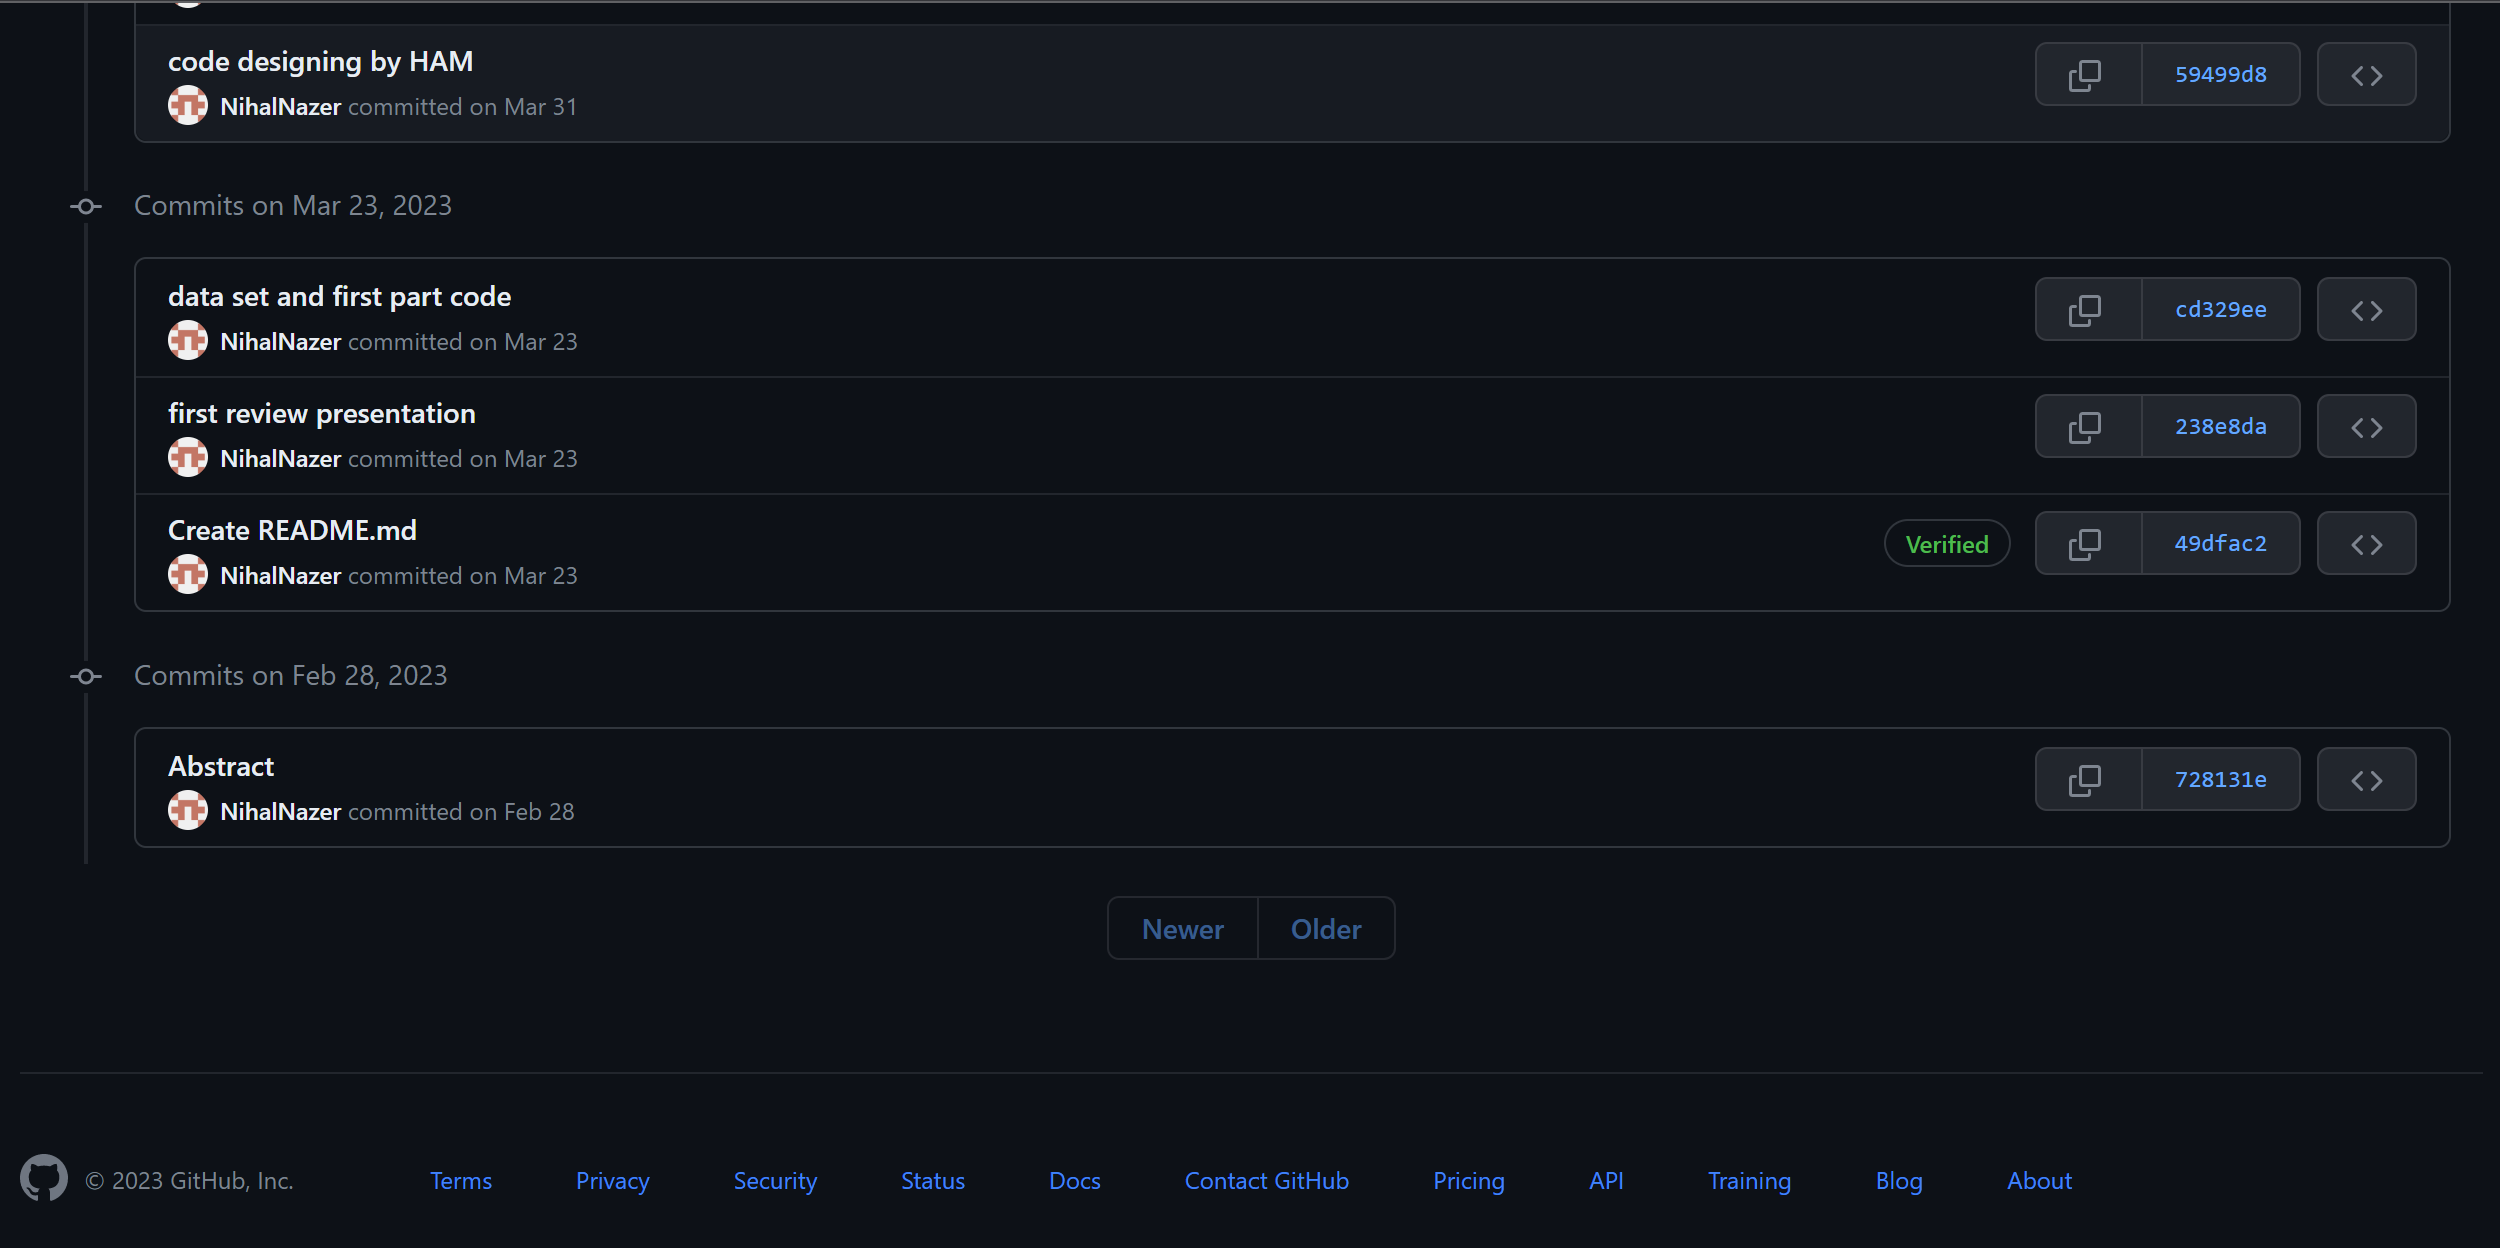
\includegraphics [width=0.9\textwidth, height=8cm]{git 3.png}
  \caption{Git 3}
  \label{fig:image}
\end{figure}

\begin{figure}[htbp]
  \centering
  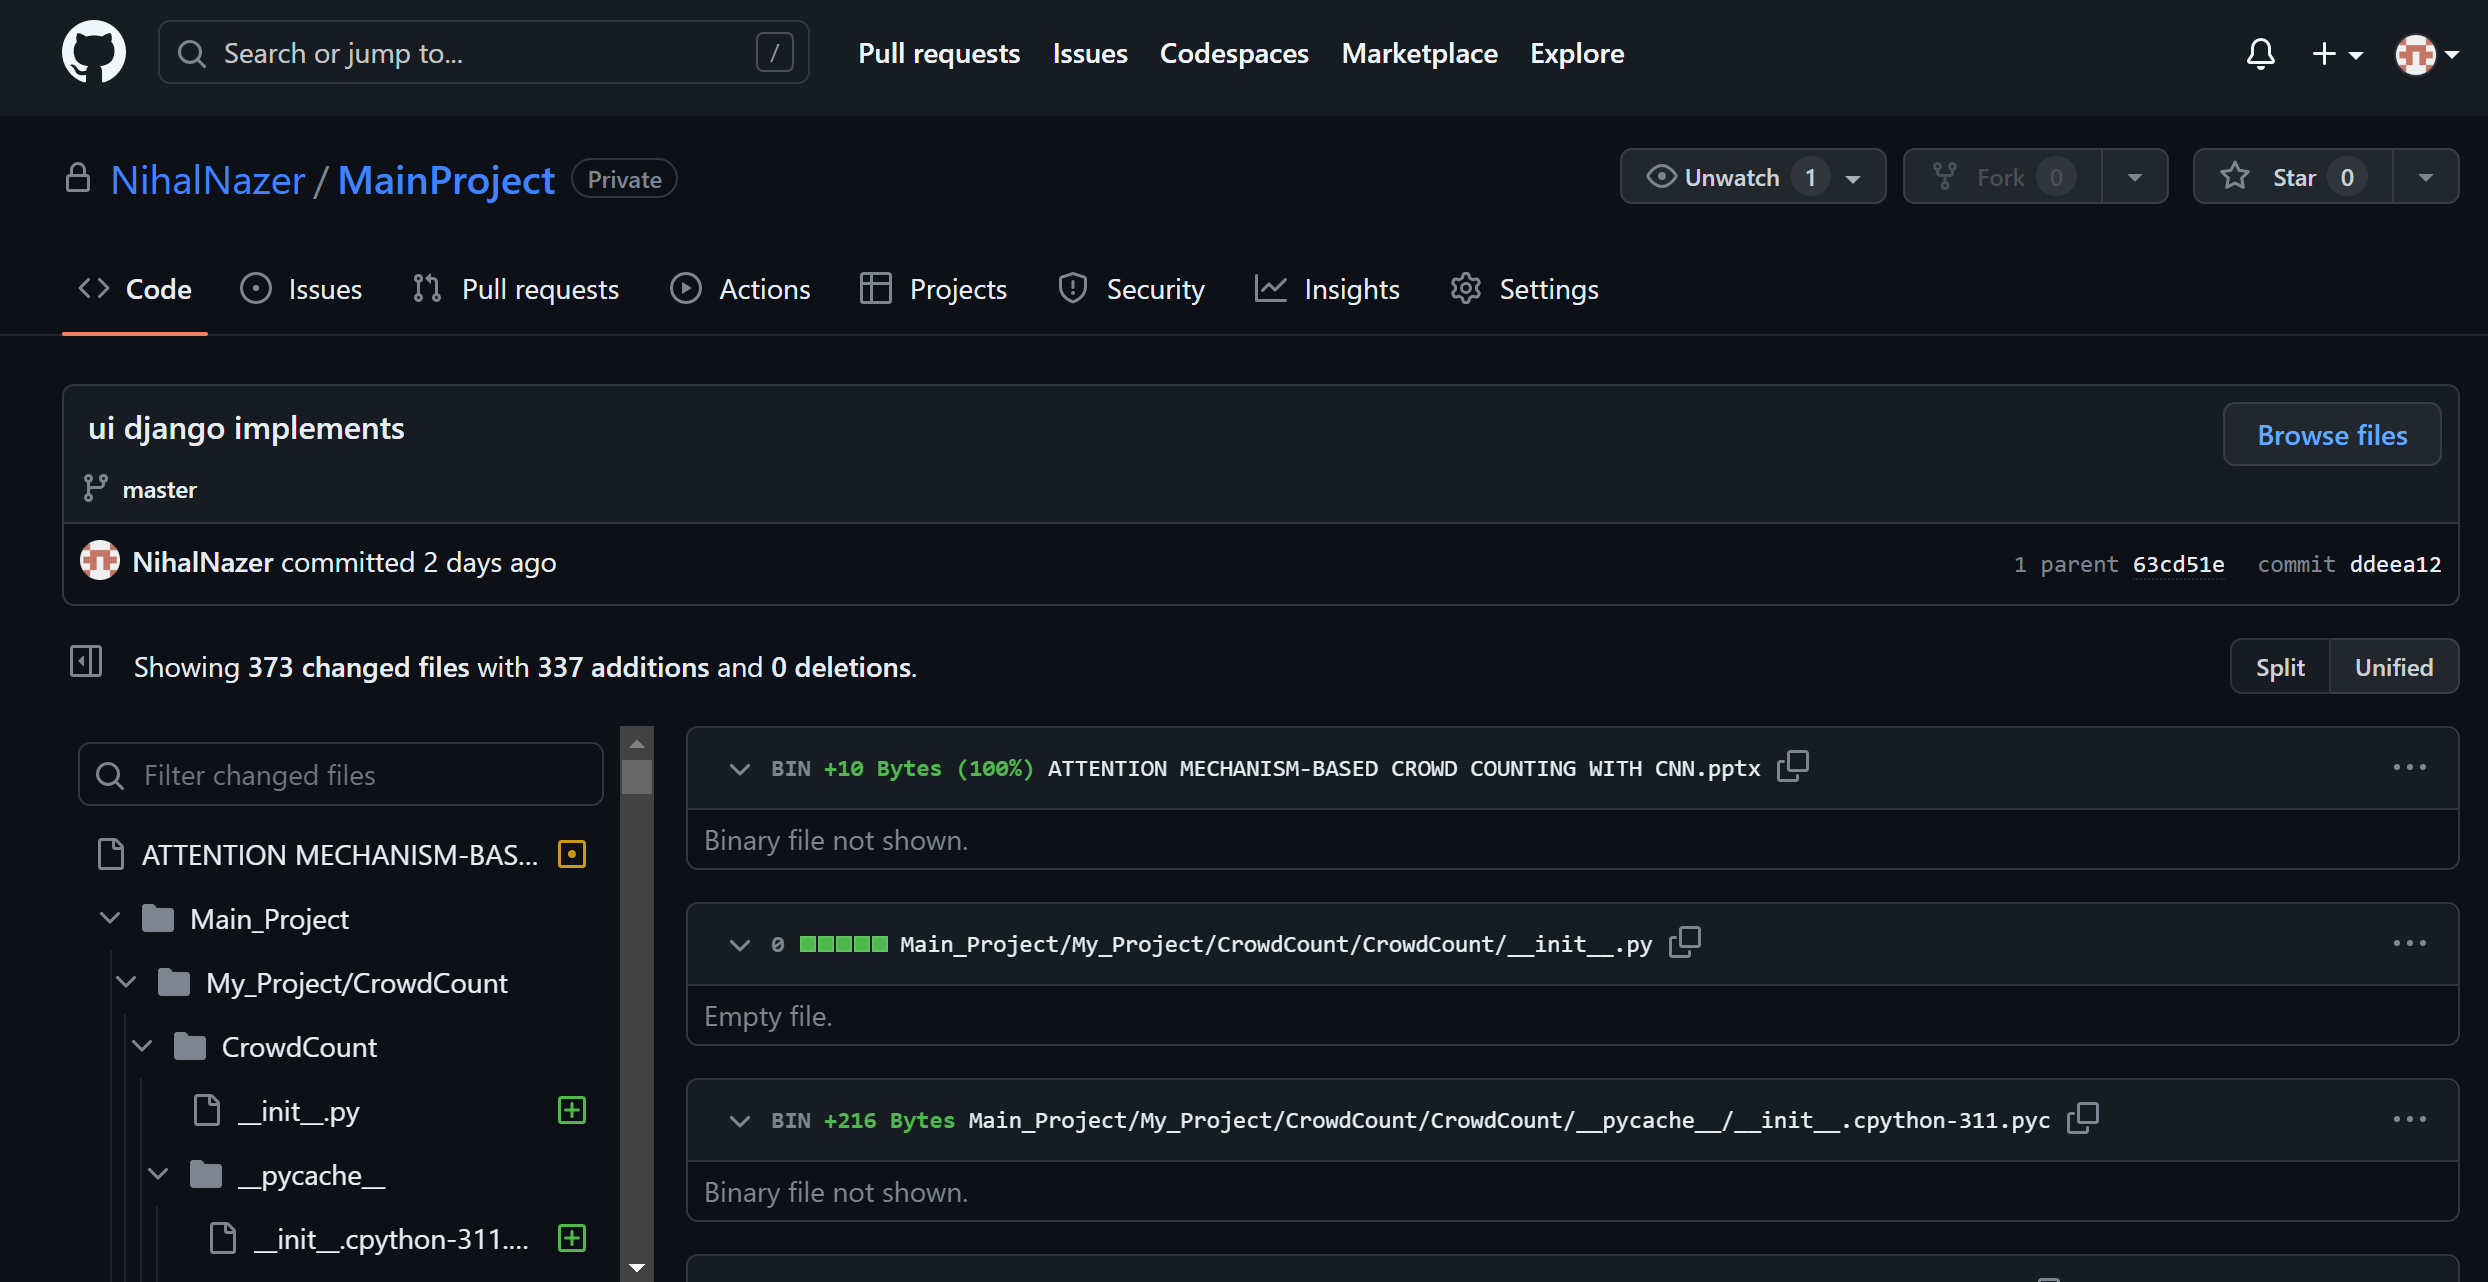
\includegraphics [width=0.9\textwidth, height=8cm]{git 4.png}
  \caption{Git 4}
  \label{fig:image}
\end{figure}

\begin{figure}[htbp]
  \centering
  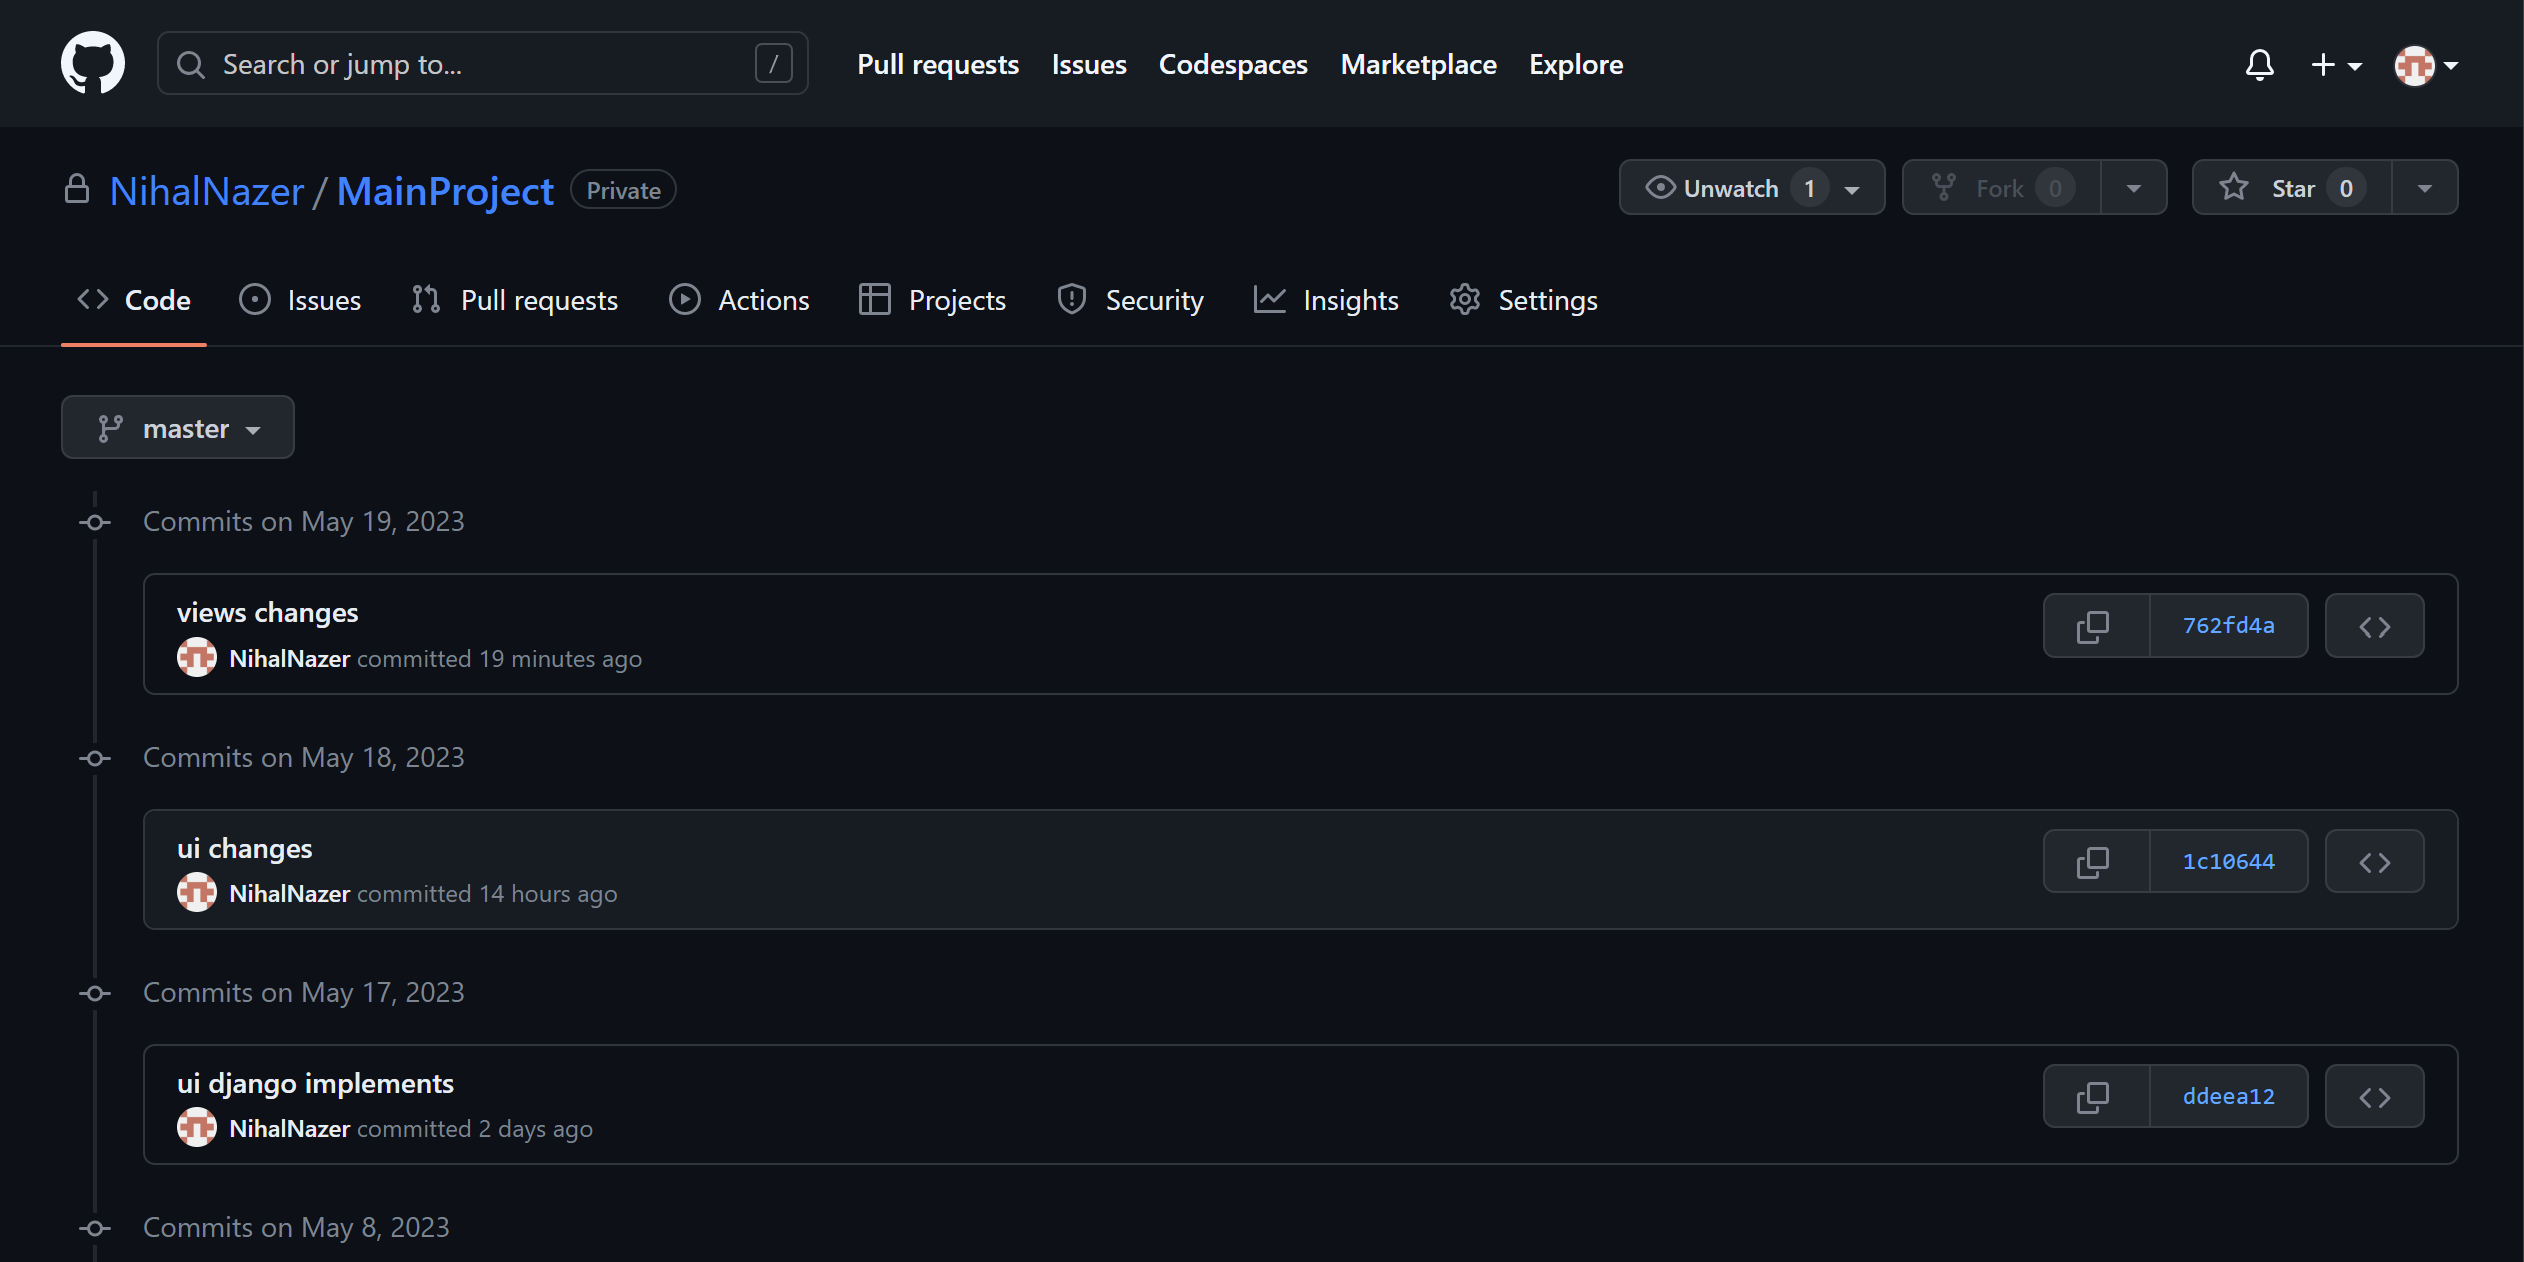
\includegraphics [width=0.9\textwidth, height=8cm]{git 5.png}
  \caption{Git 5}
  \label{fig:image}
\end{figure}




\end{document}